\documentclass[10pt,a4paper]{article}
\usepackage[margin=1.8cm]{geometry}
\usepackage{amsmath,amssymb,amsfonts,bm}
\usepackage{graphicx}
\usepackage{booktabs}
\usepackage{adjustbox}
\usepackage{float}
\usepackage{caption}
\usepackage{xcolor}
\usepackage{hyperref}
\usepackage{microtype}
\usepackage{listings}
\usepackage{tikz}
\usetikzlibrary{shapes,arrows.meta,positioning}

\definecolor{darkblue}{rgb}{0.0,0.15,0.55}
\definecolor{codegray}{rgb}{0.96,0.96,0.96}
\definecolor{codeborder}{rgb}{0.8,0.8,0.8}

\hypersetup{
    colorlinks=true,
    linkcolor=darkblue,
    citecolor=darkblue,
    urlcolor=darkblue,
    pdfauthor={RL-VMC Framework},
    pdftitle={Benchmarks de Cruce Nodal y Muestreo Puro Multi-Determinante}
}

\lstset{
    backgroundcolor=\color{codegray},
    basicstyle=\ttfamily\small,
    breaklines=true,
    frame=single,
    rulecolor=\color{codeborder},
    xleftmargin=0.5cm,
    framexleftmargin=0.3cm
}

\title{\textbf{\Large Benchmarks de Cruce Nodal y Muestreo Puro Multi-Determinante (CASSCF 1D):\\
Teoría, Implementación y Resultados Consolidados}}
\author{\textbf{RL-VMC Framework / Deep Deterministic Quantum Monte Carlo}}
\date{Noviembre 2026}

\begin{document}
\maketitle

\begin{abstract}
Este informe presenta el marco teórico formal, la formulación algorítmica y el análisis cuantitativo consolidado de 114 configuraciones evaluadas en los dos benchmarks fundamentales de muestreo MCMC puro sobre funciones de onda multiconfiguracionales congeladas (CASSCF): el cristal de Wigner fuertemente correlacionado ($N=4, g=4.0, a=0.1$) y el sistema multi-determinante $\mathrm{CAS}(6e, 6o)$ con 20 determinantes en base Hermite expandida ($N=6, g=1.0, N_{\mathrm{basis}}=256$). Se demuestra que MALA clásico colapsa debido al congelamiento topológico y a las seudo-barreras de Wigner ($D_{\mathrm{KL}}^{\mathrm{spin}} \sim 0.02 - 0.63$), mientras que el muestreador adaptativo RL-MALA con red DeepSet y recompensa CDLB erradica el bloqueo de espín ($D_{\mathrm{KL}}^{\mathrm{spin}} \sim 10^{-5} - 10^{-3}$, mejora de hasta $18,860\times$), preservando rigurosamente la energía variacional CASSCF ($\Delta E < 0.5\text{ mHa}$) y cuadruplicando la distancia de salto ($\mathrm{ESJD} > 2.4\text{ Bohr}^2$). Asimismo, se presenta la caracterización sistemática de intercambios topológicos (\texttt{flips}) en función del acoplamiento $g \in [0.1, 8.0]$ y del número de electrones $N$, demostrando aceleraciones de $50\times$ a $160\times$ en la tasa de cruces pozo-a-pozo mediante saltos colectivos de 1 paso ($25\%-55\%$), se justifica físicamente por qué las corridas preliminares con orbitales de core congelados ($n_{\mathrm{core}} > 0$) en $N \ge 6$ impidieron la cristalización de Wigner, y se documenta el protocolo de re-ejecución con estados CASSCF convergidos de espacio activo completo ($N_{\mathrm{basis}}=256, n_{\mathrm{core}}=0$).
\end{abstract}

\tableofcontents
\vspace{0.8cm}
\hrule
\vspace{0.8cm}



Este documento presenta el marco teórico, la implementación algorítmica y el análisis cuantitativo exhaustivo de los dos benchmarks fundamentales de \textbf{muestreo MCMC puro sobre funciones de onda multiconfiguracionales congeladas (CASSCF)} ejecutados en \texttt{baker}:



\begin{itemize}
\item \textbf{Benchmark 1 (\texttt{Wigner\_N4\_g4.0}):} Cristal de Wigner fuertemente correlacionado de $N=4$ electrones ($N_\uparrow=2, N_\downarrow=2, \omega=0.1, g=4.0, a=0.1$, 36 determinantes CI en base $N_{\mathrm{basis}}=32$, $E_{\mathrm{CASSCF}} = 4.1595825\text{ Ha}$).
\item \textbf{Benchmark 2 (\texttt{MultiDet\_N6\_g1.0}):} Sistema multi-determinante de $N=6$ electrones en espacio activo completo $\mathrm{CAS}(6e, 6o)$ truncado a los 20 determinantes dominantes en base expandida $N_{\mathrm{basis}}=256$ ($N_\uparrow=3, N_\downarrow=3, \omega=0.1, g=1.0, a=0.1$, $E_{\mathrm{CASSCF}} = 4.5240521\text{ Ha}$).
\end{itemize}




\vspace{0.4cm}\hrule\vspace{0.4cm}




\section{Marco Teórico: Congelamiento Topológico y Cruce de Barreras Nodales en 1D}




\subsection{Hamiltoniano Físico y Simetría Exacta de Espín}

Consideramos un sistema de $N = N_\uparrow + N_\downarrow$ electrones confinados en una trampa armónica unidimensional con interacción repulsiva de Coulomb suavizada (\textit{soft-Coulomb}):



\[
\hat{H} = \sum_{i=1}^{N} \left( -\frac{1}{2}\frac{\partial^2}{\partial x_i^2} + \frac{1}{2}\omega^2 x_i^2 \right) + \sum_{1 \le i < j \le N} \frac{g}{\sqrt{(x_i - x_j)^2 + a^2}}
\]



Dado que $\hat{H}$ es completamente independiente del espín ($\hat{H}$ conmuta con los operadores de permutación espacial y con $\hat{S}^2, \hat{S}_z$), para un sistema cerrado en espín ($N_\uparrow = N_\downarrow = N/2$) cualquier estado propio exacto o aproximación variacional invariante de espín (como RHF-CASSCF) satisface idénticamente la \textbf{simetría de densidad de un cuerpo resuelta por espín}:



\[
\rho_\uparrow^{\mathrm{exact}}(x) = \rho_\downarrow^{\mathrm{exact}}(x) = \frac{1}{2}\rho_{\mathrm{tot}}^{\mathrm{exact}}(x), \qquad \forall x \in \mathbb{R}
\]



donde la densidad normalizada a la unidad se define como $p_\sigma(x) = \rho_\sigma(x) / N_\sigma$ con $\int_{-\infty}^{\infty} p_\sigma(x)\,dx = 1$.




\subsection{Estructura Nodal y Seudo-Barreras de Wigner}

La función de onda multiconfiguracional CASSCF expandida en $M_{\mathrm{det}}$ determinantes de Slater se expresa como:



\[
\Psi_{\mathrm{CASSCF}}(\mathbf{x}_\uparrow, \mathbf{x}_\downarrow) = \sum_{k=1}^{M_{\mathrm{det}}} c_k \, \det\!\left[\phi_{k,a}^\uparrow(x_{i,\uparrow})\right]_{i,a=1}^{N_\uparrow} \det\!\left[\phi_{k,b}^\downarrow(x_{j,\downarrow})\right]_{j,b=1}^{N_\downarrow}
\]



donde cada orbital molecular activo o de core $\phi_p(x) = \sum_{n=0}^{N_{\mathrm{basis}}-1} C_{n,p}\,\chi_n^{\mathrm{HO}}(x; \omega)$ se expande en autofunciones del oscilador armónico 1D evaluadas mediante la recurrencia estable de tres términos de Hermite.



En dimensión $d=1$, la topología del espacio de configuración $\mathbb{R}^N$ presenta dos obstáculos severos para los muestreadores locales basados en gradientes:



\begin{itemize}
\item \textbf{Hiperplanos Nodales Exactos por Antisimetría de Pauli ($x_{i,\sigma} = x_{j,\sigma}$):}
\end{itemize}

   Cuando dos electrones del \textbf{mismo espín} coinciden ($x_{i,\sigma} = x_{j,\sigma}$), cada determinante se anula exactamente ($\Psi_{\mathrm{CASSCF}} = 0$). La deriva cuántica de Langevin:

\[
   \mathbf{F}_{\mathrm{Q}}(\mathbf{x}) = \nabla_{\mathbf{x}} \ln |\Psi_{\mathrm{CASSCF}}(\mathbf{x})| \sim \frac{1}{x_{i,\sigma} - x_{j,\sigma}} \to \pm\infty
\]

   diverge repulsivamente en la superficie nodal. En una propuesta difusiva estándar de tipo MALA:

\[
   \mathbf{x}' = \mathbf{x} + \tau \nabla_{\mathbf{x}} \ln |\Psi(\mathbf{x})| + \sqrt{2\tau}\,\boldsymbol{\xi}, \qquad \boldsymbol{\xi} \sim \mathcal{N}(\mathbf{0}, \mathbf{I})
\]

   la deriva cuántica empuja a los caminantes lejos del nodo; si por fluctuación gaussiana un caminante intenta cruzar el nodo con un paso $\tau$ grande, cae en regiones de alta energía o de asimetría en la razón de transición inversa $q(\mathbf{x} \mid \mathbf{x}') / q(\mathbf{x}' \mid \mathbf{x})$, desplomando la aceptación de Metropolis-Hastings.



\begin{itemize}
\item \textbf{Seudo-Barreras de Correlación de Wigner entre Espines Opuestos ($x_{i,\uparrow} \approx x_{j,\downarrow}$):}
\end{itemize}

   Aunque el principio de Pauli no prohíbe el cruce de electrones de \textbf{espín opuesto} ($x_{i,\uparrow} = x_{j,\downarrow}$), la repulsión de Coulomb $g / \sqrt{(x_i - x_j)^2 + a^2}$ junto con los determinantes excitados de correlación izquierda-derecha suprimen exponencialmente la densidad de probabilidad $|\Psi(\mathbf{x})|^2$ cuando dos electrones se superponen. Esto divide $\mathbb{R}^N$ en $N!$ \textbf{bolsillos de permutación de espín} separados por valles profundos de baja probabilidad.

   Si la cadena MCMC se inicia en un sector ordenado por espín (por ejemplo, $x_{1,\uparrow} < \dots < x_{N_\uparrow,\uparrow} < 0 < x_{1,\downarrow} < \dots < x_{N_\downarrow,\downarrow}$), el muestreador MALA clásico queda \textbf{topológicamente congelado} (\textit{broken ergodicity}): muestrea correctamente los $N$ picos espaciales de la densidad total $\rho_{\mathrm{tot}}(x)$ ($D_{\mathrm{KL}}^{\mathrm{tot}} \sim 10^{-5}$), pero es incapaz de permutar los espines entre los pozos de Wigner, produciendo una polarización espuria masiva ($\rho_\uparrow(x) \neq \rho_\downarrow(x)$, con $D_{\mathrm{KL}}^{\mathrm{spin}} \sim 0.12 - 0.63$).




\vspace{0.4cm}\hrule\vspace{0.4cm}




\section{Arquitectura RL-MALA con Actor DeepSet/SchNet y Recompensa CDLB}




\subsection{Propuesta Neuronal Equivariante (Residual MALA + Escala Adaptativa)}

El muestreador \textbf{RL-MALA} parametriza una distribución de propuesta gaussiana anisotrópica condicionada al estado actual $\mathbf{x} \in \mathbb{R}^N$ y al gradiente cuántico $\mathbf{g}(\mathbf{x}) = \nabla_{\mathbf{x}} \ln |\Psi(\mathbf{x})|$:



\[
q_\theta(\mathbf{x}' \mid \mathbf{x}) = \mathcal{N}\!\left(\mathbf{x}' \;\Big|\; \boldsymbol{\mu}_\theta(\mathbf{x}),\, \operatorname{diag}\!\big(\boldsymbol{\sigma}_\theta^2(\mathbf{x})\big)\right)
\]



donde la media y la desviación estándar por electrón combinan la física local de Langevin con una corrección neuronal no local aprendida por un Actor DeepSet con filtros continuos tipo SchNet sobre distancias interelectrónicas resueltas por espín ($r_{ij} = x_i - x_j$, canales $\uparrow\uparrow, \downarrow\downarrow, \uparrow\downarrow$):



\[
\boldsymbol{\mu}_\theta(\mathbf{x}) = \mathbf{x} + \tau\,\mathbf{g}_{\mathrm{clip}}(\mathbf{x}) + A_\mu \tanh\!\big(\mathbf{u}_\theta(\mathbf{x}, \mathbf{g})\big), \qquad
\boldsymbol{\sigma}_\theta(\mathbf{x}) = \sqrt{2\tau}\,\sigma_{\mathrm{scale}} \exp\!\big(s_\theta(\mathbf{x}, \mathbf{g})\big)
\]



Aquí:

\begin{itemize}
\item $A_\mu$ (\texttt{actor\_amplitude}) controla la amplitud física máxima del desplazamiento residual colectivo aprendido por el actor.
\item $\sigma_{\mathrm{scale}}$ (\texttt{sigma\_action\_scale}) modula la apertura estocástica de la covarianza de propuesta.
\item La aceptación exacta de Metropolis-Hastings preserva el balance detallado estricto respecto a $\pi(\mathbf{x}) \propto |\Psi_{\mathrm{CASSCF}}(\mathbf{x})|^2$:
\[
  \alpha_\theta(\mathbf{x} \to \mathbf{x}') = \min\!\left\{1,\, \frac{|\Psi_{\mathrm{CASSCF}}(\mathbf{x}')|^2 \, q_\theta(\mathbf{x} \mid \mathbf{x}')}{|\Psi_{\mathrm{CASSCF}}(\mathbf{x})|^2 \, q_\theta(\mathbf{x}' \mid \mathbf{x})}\right\}
\]

\end{itemize}




\subsection{Recompensa CDLB (\textit{Clipped Detailed-Balance Log-Barrier}) con Exploración Entrópica}

Para evitar que el actor colapse a pasos triviales ($\mathbf{x}' \approx \mathbf{x}$) o proponga saltos no reversibles que anulen $q_\theta(\mathbf{x} \mid \mathbf{x}')$, entrenamos mediante \textbf{TD3 (\textit{Twin Delayed Deep Deterministic Policy Gradient})} maximizando la recompensa \textbf{CDLB}:



\[
r_{\mathrm{CDLB}}(\mathbf{x}, \mathbf{x}') = \alpha_\theta(\mathbf{x} \to \mathbf{x}') \cdot \ln\!\left(1 + \frac{\|\mathbf{x}' - \mathbf{x}\|_{\mathrm{clip}}^2}{\tau}\right) - \lambda_{\mathrm{pen}}\big(1 - \alpha_\theta(\mathbf{x} \to \mathbf{x}')\big) - \alpha_{\mathrm{ent}} \ln q_\theta(\mathbf{x}' \mid \mathbf{x})
\]



Esta formulación logra tres efectos simultáneos:

\begin{itemize}
\item \textbf{Impulso de salto colectivo:} El término $\alpha_\theta \ln(1 + \|\Delta \mathbf{x}\|^2 / \tau)$ premia desplazamientos largos en el espacio de configuración que mantengan alta probabilidad de aceptación.
\item \textbf{Penalización de rechazo ($\lambda_{\mathrm{pen}}$):} Evita que el actor proponga saltos demasiado agresivos hacia el exterior del pozo armónico.
\item \textbf{Exploración calibrada ($-\alpha_{\mathrm{ent}} \ln q_\theta$):} Incentiva al actor a ensanchar selectivamente $\boldsymbol{\sigma}_\theta(\mathbf{x})$ cuando dos electrones de espín opuesto o igual se aproximan a una barrera nodal, permitiendo \textbf{saltar por encima del valle nodal} de un bolsillo de permutación a otro en un solo paso colectivo.
\end{itemize}




\vspace{0.4cm}\hrule\vspace{0.4cm}




\section{Protocolo Experimental e Implementación Computacional}



Para garantizar una comparación justa, reproducible y libre de sesgos entre MALA y RL-MALA:



\begin{itemize}
\item \textbf{Aislamiento de la Función de Onda (\texttt{--ansatz\_type casscf\_npz --no-casscf\_trainable}):}
\end{itemize}

   Ambos métodos muestrean exactamente el mismo estado multiconfiguracional congelado \texttt{casscf\_state.npz}. No se modifica ningún parámetro del ansatz durante el entrenamiento ni durante la evaluación.

\begin{itemize}
\item \textbf{Inicialización Simétrica durante el Entrenamiento RL (\texttt{--init\_mode symmetric\_gaussian --init\_std 3.0}):}
\end{itemize}

   Durante los $6,000$ barridos de entrenamiento TD3 (\texttt{--train\_mode rl\_only}, $N_{\mathrm{walkers}}=128$, burn-in inicial de $2,000$ pasos), los caminantes se inicializan con una distribución gaussiana simétrica para poblar el \textit{replay buffer} en todos los sectores de permutación de espín sin sesgo espacial.

\begin{itemize}
\item \textbf{Prueba de Estrés de Cruce Nodal en Producción (\texttt{--eval\_init\_mode spin\_ordered\_offset}):}
\end{itemize}

   En la fase de evaluación de producción ($N_{\mathrm{chains}}=3$ cadenas independientes, $N_{\mathrm{walkers}}=128$, \texttt{eval\_burn\_in = 200}, \texttt{measure\_steps = 40,000}), tanto MALA como RL-MALA se inicializan deliberadamente en una configuración \textbf{totalmente polarizada por espín}:

\begin{itemize}
\item Todos los electrones $\uparrow$ en el semieje izquierdo ($x_{i,\uparrow} < 0$).
\item Todos los electrones $\downarrow$ en el semieje derecho ($x_{j,\downarrow} > 0$).
\end{itemize}

   Un muestreador ergódico capaz de cruzar barreras nodales debe restaurar rápidamente la simetría exacta $\rho_\uparrow(x) = \rho_\downarrow(x) = \frac{1}{2}\rho_{\mathrm{tot}}(x)$, haciendo que la divergencia de Kullback-Leibler promedio de espín:

\[
   D_{\mathrm{KL}}^{\mathrm{spin}} = \frac{1}{2}\Big[D_{\mathrm{KL}}\!\big(p_\uparrow^{\mathrm{MCMC}} \parallel p_\uparrow^{\mathrm{CASSCF}}\big) + D_{\mathrm{KL}}\!\big(p_\downarrow^{\mathrm{MCMC}} \parallel p_\downarrow^{\mathrm{CASSCF}}\big)\Big]
\]

   tienda asintóticamente a cero ($D_{\mathrm{KL}}^{\mathrm{spin}} \to 10^{-5} - 10^{-3}$). Por el contrario, si el muestreador queda atrapado en su sector topológico inicial, $D_{\mathrm{KL}}^{\mathrm{spin}}$ permanece estancado en $\mathcal{O}(0.1 - 0.6)$.




\vspace{0.4cm}\hrule\vspace{0.4cm}




\section{Resultados del Benchmark 1: \texttt{Wigner\_N4\_g4.0} ($N=4, \omega=0.1, g=4.0$)}




\subsection{Sistema de Referencia}

\begin{itemize}
\item \textbf{Parámetros físicos:} $N=4$ ($N_\uparrow=2, N_\downarrow=2$), $\omega=0.1$, $g=4.0$, $a=0.1$.
\item \textbf{Referencia CASSCF:} \texttt{cas\_n4\_g4\_omega0.1\_soft0.1\_b32\_c0-a4} ($N_{\mathrm{core}}=0, N_{\mathrm{active}}=4 \implies 36$ determinantes, base $N_{\mathrm{basis}}=32$), con energía exacta $E_{\mathrm{CASSCF}} = \mathbf{4.1595825\text{ Ha}}$.
\item \textbf{Régimen físico:} Cristal de Wigner de 4 picos bien separados en $x \approx \pm 2.2, \pm 6.8\text{ Bohr}$.
\end{itemize}




\subsection{Benchmark Inicial en Baker (Grilla Compacta, 16 Modelos)}



\begin{table}[H]
\centering
\begin{adjustbox}{max width=\textwidth}
\begin{tabular}{lcccccccccccc}
\toprule
\textbf{Modelo} & \textbf{$\tau$} & \textbf{$A_\mu$} & \textbf{$\lambda_{\mathrm{pen}}$} & \textbf{$\langle E \rangle \pm \mathrm{SE}(E)$ (Ha)} & \textbf{$\Delta E$ (mHa)} & \textbf{Aceptación} & \textbf{ESJD ($\text{Bohr}^2$)} & \textbf{$\tau_{\mathrm{int}}(E)$} & \textbf{$\tau_{\mathrm{int}}(x)$} & \textbf{$\mathrm{ESS/s}$ ($\text{s}^{-1}$)} & \textbf{$D_{\mathrm{KL}}^{\mathrm{tot}}$} & \textbf{$D_{\mathrm{KL}}^{\mathrm{spin}}$ (Cruce Nodal)} \\
\midrule
\texttt{MALA\_tau0.04} & 0.04 & --- & --- & $4.160448 \pm 0.000557$ & $+0.87$ & $94.4\%$ & $0.291$ & $106.89 \pm 16.46$ & $2280.1$ & $1,141$ & $2.52 \times 10^{-4}$ & $0.62609$ \\
\texttt{MALA\_tau0.08} & 0.08 & --- & --- & $4.160328 \pm 0.000338$ & $+0.75$ & $90.2\%$ & $0.556$ & $39.67 \pm 3.85$ & $2219.9$ & $3,081$ & $1.10 \times 10^{-4}$ & $0.58777$ \\
\texttt{MALA\_tau0.10} & 0.10 & --- & --- & $4.159480 \pm 0.000237$ & $-0.10$ & $88.5\%$ & $0.685$ & $19.48 \pm 1.38$ & $2090.6$ & $6,267$ & $1.52 \times 10^{-4}$ & $0.52840$ \\
\textbf{\texttt{MALA\_tau0.12} (Mejor MALA)} & \textbf{0.12} & --- & --- & \textbf{$4.159500 \pm 0.000180$} & \textbf{$-0.08$} & \textbf{$87.1\%$} & \textbf{$0.813$} & \textbf{$11.07 \pm 0.62$} & \textbf{$1855.3$} & \textbf{$11,033$} & \textbf{$1.11 \times 10^{-4}$} & \textbf{$0.46867$} \\
\texttt{RL\_MALA\_tau0.08\_amp0.10\_pen0.15\_sig1.1} & 0.08 & 0.10 & 0.15 & $4.159819 \pm 0.000143$ & $+0.24$ & $55.6\%$ & $1.688$ & $6.96 \pm 0.32$ & $886.4$ & $11,932$ & $5.25 \times 10^{-5}$ & $0.03651$ \\
\textbf{\texttt{RL\_MALA\_tau0.08\_amp0.10\_pen0.25\_sig1.1}} & \textbf{0.08} & \textbf{0.10} & \textbf{0.25} & \textbf{$4.159843 \pm 0.000130$} & \textbf{$+0.26$} & \textbf{$47.7\%$} & \textbf{$2.020$} & \textbf{$5.79 \pm 0.24$} & \textbf{$546.5$} & \textbf{$14,264$} & \textbf{$3.18 \times 10^{-5}$} & \textbf{$0.01564$} \\
\texttt{RL\_MALA\_tau0.08\_amp0.15\_pen0.15\_sig1.1} & 0.08 & 0.15 & 0.15 & $4.159553 \pm 0.000175$ & $-0.03$ & $36.0\%$ & $1.807$ & $10.43 \pm 0.56$ & $533.1$ & $7,953$ & $3.65 \times 10^{-5}$ & $0.01851$ \\
\texttt{RL\_MALA\_tau0.08\_amp0.15\_pen0.25\_sig1.1} & 0.08 & 0.15 & 0.25 & $4.159609 \pm 0.000161$ & $+0.03$ & $41.3\%$ & $1.741$ & $8.90 \pm 0.45$ & $760.6$ & $9,225$ & $4.54 \times 10^{-5}$ & $0.04425$ \\
\texttt{RL\_MALA\_tau0.08\_amp0.25\_pen0.15\_sig1.1} & 0.08 & 0.25 & 0.15 & $4.158805 \pm 0.000605$ & $-0.78$ & $10.4\%$ & $0.916$ & $131.69 \pm 16.01$ & $945.9$ & $627$ & $1.50 \times 10^{-4}$ & $0.03699$ \\
\texttt{RL\_MALA\_tau0.08\_amp0.25\_pen0.25\_sig1.1} & 0.08 & 0.25 & 0.25 & $4.159944 \pm 0.000592$ & $+0.36$ & $10.5\%$ & $0.930$ & $122.90 \pm 14.37$ & $1017.1$ & $669$ & $1.41 \times 10^{-4}$ & $0.07855$ \\
\texttt{RL\_MALA\_tau0.10\_amp0.10\_pen0.15\_sig1.1} & 0.10 & 0.10 & 0.15 & $4.159624 \pm 0.000149$ & $+0.04$ & $62.0\%$ & $1.564$ & $7.60 \pm 0.36$ & $1150.7$ & $10,889$ & $3.54 \times 10^{-5}$ & $0.09772$ \\
\textbf{\texttt{RL\_MALA\_tau0.10\_amp0.10\_pen0.25\_sig1.1} (Óptimo)} & \textbf{0.10} & \textbf{0.10} & \textbf{0.25} & \textbf{$4.159469 \pm 0.000126$} & \textbf{$-0.11$} & \textbf{$45.8\%$} & \textbf{$2.156$} & \textbf{$5.43 \pm 0.22$} & \textbf{$568.5$} & \textbf{$15,078$} & \textbf{$3.05 \times 10^{-5}$} & \textbf{$0.00958$} \\
\texttt{RL\_MALA\_tau0.10\_amp0.15\_pen0.15\_sig1.1} & 0.10 & 0.15 & 0.15 & $4.159710 \pm 0.000155$ & $+0.13$ & $38.4\%$ & $1.908$ & $8.13 \pm 0.40$ & $597.2$ & $10,084$ & $3.26 \times 10^{-5}$ & $0.01451$ \\
\texttt{RL\_MALA\_tau0.10\_amp0.15\_pen0.25\_sig1.1} & 0.10 & 0.15 & 0.25 & $4.159626 \pm 0.000178$ & $+0.04$ & $33.0\%$ & $1.727$ & $10.90 \pm 0.61$ & $554.7$ & $7,584$ & $4.08 \times 10^{-5}$ & $0.00998$ \\
\texttt{RL\_MALA\_tau0.10\_amp0.25\_pen0.15\_sig1.1} & 0.10 & 0.25 & 0.15 & $4.159643 \pm 0.000147$ & $+0.06$ & $65.0\%$ & $1.594$ & $7.37 \pm 0.35$ & $1224.2$ & $11,175$ & $2.91 \times 10^{-5}$ & $0.08826$ \\
\texttt{RL\_MALA\_tau0.10\_amp0.25\_pen0.25\_sig1.1} & 0.10 & 0.25 & 0.25 & $4.159500 \pm 0.000143$ & $-0.08$ & $54.2\%$ & $1.802$ & $7.01 \pm 0.32$ & $893.7$ & $11,769$ & $3.41 \times 10^{-5}$ & $0.02975$ \\
\bottomrule
\end{tabular}
\end{adjustbox}
\end{table}



\subsection{Hallazgos de la Exploración Inicial en Baker}

\begin{itemize}
\item \textbf{Ruptura del bloqueo de espín ($49\times$ a $65\times$ menor $D_{\mathrm{KL}}^{\mathrm{spin}}$):} Todos los modelos MALA quedan severamente polarizados ($D_{\mathrm{KL}}^{\mathrm{spin}} \in [0.469, 0.626]$), mientras que \texttt{RL\_MALA\_tau0.10\_amp0.10\_pen0.25\_sig1.1} reduce $D_{\mathrm{KL}}^{\mathrm{spin}}$ a \textbf{$0.00958$} (una mejora de \textbf{$48.9\times$} frente al mejor MALA y \textbf{$65.4\times$} frente a MALA $\tau=0.04$).
\item \textbf{Aceleración real de reloj ($\mathrm{ESS/s}$):} Pese al costo adicional de evaluar la red DeepSet en cada paso, \texttt{RL\_MALA\_tau0.10\_amp0.10\_pen0.25\_sig1.1} alcanza \textbf{$\mathbf{15,078\text{ s}^{-1}}$}, superando al mejor MALA ($11,033\text{ s}^{-1}$) en un \textbf{+$36.7\%$ neto} y reduciendo $\tau_{\mathrm{int}}(E)$ de $11.07$ a \textbf{$5.43$ pasos} ($2.04\times$ menor) y la autocorrelación espacial $\tau_{\mathrm{int}}(x)$ de $1855.3$ a \textbf{$568.5$ pasos} ($3.26\times$ menor).
\item \textbf{Sensibilidad a $A_\mu$ en acoplamiento fuerte ($g=4.0$):} Cuando $A_\mu = 0.25$ y $\tau=0.08$, el salto propuesto excede el ancho de los bolsillos de Wigner, reduciendo la aceptación a $\sim 10.4\%$. En cambio, el rango \textbf{$A_\mu \in [0.10, 0.15]$ con $\lambda_{\mathrm{pen}} = 0.25$} mantiene la aceptación exactamente en el régimen óptimo de transporte no local ($45\% - 55\%$).
\end{itemize}




\subsection{Nueva Exploración Sistemática en Ayler (Grilla Completa de 41 Modelos)}

Para explorar si pasos temporales mayores ($\tau \ge 0.14$) logran un mayor rendimiento sin romper el transporte cuántico, se ejecutó en Ayler una grilla complementaria de 41 modelos (5 MALA + 36 RL-MALA) con:

\begin{itemize}
\item MALA: $\tau \in \{0.06, 0.14, 0.16, 0.20, 0.25\}$
\item RL-MALA: $\tau \in \{0.10, 0.12, 0.14\}$, $A_\mu \in \{0.06, 0.08, 0.12, 0.18\}$, $\lambda_{\mathrm{pen}} \in \{0.20, 0.30, 0.40\}$, $\sigma_{\mathrm{sc}} = 1.15$.
\end{itemize}



\begin{table}[H]
\centering
\begin{adjustbox}{max width=\textwidth}
\begin{tabular}{lcccccccccccc}
\toprule
\textbf{Modelo} & \textbf{$\tau$} & \textbf{$A_\mu$} & \textbf{$\lambda_{\mathrm{pen}}$} & \textbf{$\sigma_{\mathrm{sc}}$} & \textbf{$\langle E \rangle \pm \mathrm{SE}(E)$ (Ha)} & \textbf{$\Delta E$ (mHa)} & \textbf{Aceptación} & \textbf{ESJD ($\text{Bohr}^2$)} & \textbf{$\tau_{\mathrm{int}}(E)$} & \textbf{$\mathrm{ESS/s}$ ($\text{s}^{-1}$)} & \textbf{$D_{\mathrm{KL}}^{\mathrm{tot}}$} & \textbf{$D_{\mathrm{KL}}^{\mathrm{spin}}$ (Cruce Nodal)} \\
\midrule
\texttt{MALA\_tau0.06} & 0.06 & --- & --- & --- & $4.160265 \pm 0.000422$ & $+0.68$ & 91.0\% & 0.428 & 26.14 & 6,579 & 7.96e-06 & \textbf{3.2632} \\
\texttt{MALA\_tau0.14} & 0.14 & --- & --- & --- & $4.160030 \pm 0.000239$ & $+0.45$ & 86.1\% & 0.935 & 9.62 & 17,776 & 5.02e-06 & \textbf{0.7976} \\
\texttt{MALA\_tau0.16} & 0.16 & --- & --- & --- & $4.159943 \pm 0.000231$ & $+0.36$ & 85.1\% & 1.054 & 8.92 & 19,007 & 5.18e-06 & \textbf{0.8668} \\
\texttt{MALA\_tau0.20} & 0.20 & --- & --- & --- & $4.160000 \pm 0.000210$ & $+0.42$ & 83.3\% & 1.284 & 7.46 & 22,639 & 4.30e-06 & \textbf{0.7095} \\
\texttt{MALA\_tau0.25} & 0.25 & --- & --- & --- & $4.159716 \pm 0.000189$ & $+0.13$ & 81.3\% & 1.559 & 6.07 & 28,147 & 3.57e-06 & \textbf{0.6265} \\
\textbf{\texttt{RL\_MALA\_tau0.14\_amp0.12\_pen0.20\_sig1.15}} & 0.14 & 0.12 & 0.20 & 1.15 & $4.159816 \pm 0.000170$ & $+0.23$ & 39.7\% & 2.424 & 4.82 & 3,192,206 & 8.35e-06 & \textbf{3.9233e-03} \\
\textbf{\texttt{RL\_MALA\_tau0.14\_amp0.18\_pen0.40\_sig1.15}} & 0.14 & 0.18 & 0.40 & 1.15 & $4.159727 \pm 0.000177$ & $+0.14$ & 38.7\% & 2.358 & 5.28 & 2,909,093 & 8.70e-06 & \textbf{4.0297e-03} \\
\textbf{\texttt{RL\_MALA\_tau0.14\_amp0.06\_pen0.20\_sig1.15}} & 0.14 & 0.06 & 0.20 & 1.15 & $4.159790 \pm 0.000172$ & $+0.21$ & 40.3\% & 2.463 & 4.87 & 3,157,276 & 7.66e-06 & \textbf{4.4769e-03} \\
\texttt{RL\_MALA\_tau0.14\_amp0.08\_pen0.40\_sig1.15} & 0.14 & 0.08 & 0.40 & 1.15 & $4.159715 \pm 0.000167$ & $+0.13$ & 40.2\% & 2.454 & 4.68 & 3,283,711 & 9.16e-06 & 5.1001e-03 \\
\texttt{RL\_MALA\_tau0.14\_amp0.06\_pen0.40\_sig1.15} & 0.14 & 0.06 & 0.40 & 1.15 & $4.159863 \pm 0.000169$ & $+0.28$ & 40.3\% & 2.463 & 4.78 & 3,211,878 & 8.75e-06 & 5.3106e-03 \\
\texttt{RL\_MALA\_tau0.14\_amp0.08\_pen0.30\_sig1.15} & 0.14 & 0.08 & 0.30 & 1.15 & $4.159724 \pm 0.000168$ & $+0.14$ & 40.2\% & 2.452 & 4.77 & 3,221,036 & 8.42e-06 & 5.3708e-03 \\
\texttt{RL\_MALA\_tau0.14\_amp0.06\_pen0.30\_sig1.15} & 0.14 & 0.06 & 0.30 & 1.15 & $4.159856 \pm 0.000170$ & $+0.27$ & 40.3\% & 2.463 & 4.93 & 3,120,012 & 8.15e-06 & 5.7371e-03 \\
\texttt{RL\_MALA\_tau0.14\_amp0.12\_pen0.30\_sig1.15} & 0.14 & 0.12 & 0.30 & 1.15 & $4.159752 \pm 0.000173$ & $+0.17$ & 39.7\% & 2.423 & 5.05 & 3,039,889 & 7.43e-06 & 5.7669e-03 \\
\texttt{RL\_MALA\_tau0.14\_amp0.12\_pen0.40\_sig1.15} & 0.14 & 0.12 & 0.40 & 1.15 & $4.159873 \pm 0.000171$ & $+0.29$ & 39.7\% & 2.424 & 4.84 & 3,177,782 & 8.32e-06 & 6.7477e-03 \\
\texttt{RL\_MALA\_tau0.14\_amp0.18\_pen0.20\_sig1.15} & 0.14 & 0.18 & 0.20 & 1.15 & $4.159712 \pm 0.000178$ & $+0.13$ & 38.7\% & 2.359 & 5.35 & 2,876,357 & 9.14e-06 & 6.8302e-03 \\
\texttt{RL\_MALA\_tau0.14\_amp0.18\_pen0.30\_sig1.15} & 0.14 & 0.18 & 0.30 & 1.15 & $4.159792 \pm 0.000175$ & $+0.21$ & 38.7\% & 2.359 & 5.07 & 3,031,764 & 1.03e-05 & 7.0373e-03 \\
\texttt{RL\_MALA\_tau0.12\_amp0.06\_pen0.40\_sig1.15} & 0.12 & 0.06 & 0.40 & 1.15 & $4.159827 \pm 0.000181$ & $+0.24$ & 43.5\% & 2.348 & 5.45 & 2,826,151 & 8.48e-06 & 7.2955e-03 \\
\texttt{RL\_MALA\_tau0.14\_amp0.08\_pen0.20\_sig1.15} & 0.14 & 0.08 & 0.20 & 1.15 & $4.159861 \pm 0.000170$ & $+0.28$ & 40.2\% & 2.452 & 4.83 & 3,182,417 & 9.38e-06 & 8.5752e-03 \\
\texttt{RL\_MALA\_tau0.12\_amp0.08\_pen0.30\_sig1.15} & 0.12 & 0.08 & 0.30 & 1.15 & $4.159942 \pm 0.000190$ & $+0.36$ & 43.3\% & 2.335 & 6.04 & 2,655,834 & 6.42e-06 & 8.7031e-03 \\
\texttt{RL\_MALA\_tau0.12\_amp0.12\_pen0.30\_sig1.15} & 0.12 & 0.12 & 0.30 & 1.15 & $4.159891 \pm 0.000184$ & $+0.31$ & 42.7\% & 2.300 & 5.53 & 2,788,411 & 7.77e-06 & 9.5868e-03 \\
\texttt{RL\_MALA\_tau0.12\_amp0.18\_pen0.30\_sig1.15} & 0.12 & 0.18 & 0.30 & 1.15 & $4.159863 \pm 0.000180$ & $+0.28$ & 41.4\% & 2.227 & 5.38 & 2,853,829 & 7.19e-06 & 9.6726e-03 \\
\texttt{RL\_MALA\_tau0.12\_amp0.12\_pen0.20\_sig1.15} & 0.12 & 0.12 & 0.20 & 1.15 & $4.159754 \pm 0.000178$ & $+0.17$ & 42.7\% & 2.300 & 5.39 & 2,852,227 & 8.76e-06 & 9.8037e-03 \\
\texttt{RL\_MALA\_tau0.12\_amp0.18\_pen0.20\_sig1.15} & 0.12 & 0.18 & 0.20 & 1.15 & $4.159928 \pm 0.000177$ & $+0.35$ & 41.4\% & 2.225 & 5.27 & 2,921,047 & 8.23e-06 & 1.0127e-02 \\
\texttt{RL\_MALA\_tau0.12\_amp0.06\_pen0.30\_sig1.15} & 0.12 & 0.06 & 0.30 & 1.15 & $4.159827 \pm 0.000177$ & $+0.24$ & 43.5\% & 2.348 & 5.24 & 2,947,635 & 6.88e-06 & 1.0640e-02 \\
\texttt{RL\_MALA\_tau0.12\_amp0.06\_pen0.20\_sig1.15} & 0.12 & 0.06 & 0.20 & 1.15 & $4.159746 \pm 0.000173$ & $+0.16$ & 43.5\% & 2.347 & 5.03 & 3,055,738 & 7.99e-06 & 1.0814e-02 \\
\texttt{RL\_MALA\_tau0.12\_amp0.12\_pen0.40\_sig1.15} & 0.12 & 0.12 & 0.40 & 1.15 & $4.159840 \pm 0.000182$ & $+0.26$ & 42.7\% & 2.300 & 5.49 & 2,845,377 & 8.66e-06 & 1.2402e-02 \\
\texttt{RL\_MALA\_tau0.12\_amp0.08\_pen0.20\_sig1.15} & 0.12 & 0.08 & 0.20 & 1.15 & $4.159884 \pm 0.000182$ & $+0.30$ & 43.3\% & 2.336 & 5.65 & 2,743,630 & 8.37e-06 & 1.2454e-02 \\
\texttt{RL\_MALA\_tau0.12\_amp0.08\_pen0.40\_sig1.15} & 0.12 & 0.08 & 0.40 & 1.15 & $4.160103 \pm 0.000181$ & $+0.52$ & 43.3\% & 2.336 & 5.37 & 2,863,085 & 8.04e-06 & 1.3608e-02 \\
\texttt{RL\_MALA\_tau0.12\_amp0.18\_pen0.40\_sig1.15} & 0.12 & 0.18 & 0.40 & 1.15 & $4.159843 \pm 0.000180$ & $+0.26$ & 41.4\% & 2.226 & 5.44 & 2,822,286 & 8.45e-06 & 1.4541e-02 \\
\texttt{RL\_MALA\_tau0.10\_amp0.06\_pen0.30\_sig1.15} & 0.10 & 0.06 & 0.30 & 1.15 & $4.159828 \pm 0.000179$ & $+0.25$ & 47.2\% & 2.191 & 5.49 & 2,806,272 & 6.16e-06 & 1.4947e-02 \\
\texttt{RL\_MALA\_tau0.10\_amp0.06\_pen0.40\_sig1.15} & 0.10 & 0.06 & 0.40 & 1.15 & $4.159851 \pm 0.000186$ & $+0.27$ & 47.2\% & 2.191 & 5.74 & 2,685,668 & 6.91e-06 & 1.5605e-02 \\
\texttt{RL\_MALA\_tau0.10\_amp0.06\_pen0.20\_sig1.15} & 0.10 & 0.06 & 0.20 & 1.15 & $4.159946 \pm 0.000192$ & $+0.36$ & 47.2\% & 2.190 & 6.19 & 2,534,490 & 6.55e-06 & 1.6343e-02 \\
\texttt{RL\_MALA\_tau0.10\_amp0.08\_pen0.30\_sig1.15} & 0.10 & 0.08 & 0.30 & 1.15 & $4.159730 \pm 0.000179$ & $+0.15$ & 47.0\% & 2.176 & 5.47 & 2,810,577 & 6.03e-06 & 1.7374e-02 \\
\texttt{RL\_MALA\_tau0.10\_amp0.08\_pen0.40\_sig1.15} & 0.10 & 0.08 & 0.40 & 1.15 & $4.159764 \pm 0.000181$ & $+0.18$ & 46.9\% & 2.177 & 5.59 & 2,754,852 & 6.60e-06 & 1.8168e-02 \\
\texttt{RL\_MALA\_tau0.10\_amp0.08\_pen0.20\_sig1.15} & 0.10 & 0.08 & 0.20 & 1.15 & $4.159941 \pm 0.000184$ & $+0.36$ & 46.9\% & 2.176 & 5.66 & 2,716,887 & 6.93e-06 & 1.9430e-02 \\
\texttt{RL\_MALA\_tau0.10\_amp0.18\_pen0.30\_sig1.15} & 0.10 & 0.18 & 0.30 & 1.15 & $4.159754 \pm 0.000190$ & $+0.17$ & 44.4\% & 2.047 & 5.89 & 2,608,061 & 7.24e-06 & 1.9507e-02 \\
\texttt{RL\_MALA\_tau0.10\_amp0.12\_pen0.30\_sig1.15} & 0.10 & 0.12 & 0.30 & 1.15 & $4.159909 \pm 0.000183$ & $+0.33$ & 46.1\% & 2.136 & 5.71 & 2,692,080 & 6.22e-06 & 1.9513e-02 \\
\texttt{RL\_MALA\_tau0.10\_amp0.12\_pen0.40\_sig1.15} & 0.10 & 0.12 & 0.40 & 1.15 & $4.159848 \pm 0.000183$ & $+0.27$ & 46.1\% & 2.136 & 5.58 & 2,758,992 & 6.78e-06 & 2.2136e-02 \\
\texttt{RL\_MALA\_tau0.10\_amp0.12\_pen0.20\_sig1.15} & 0.10 & 0.12 & 0.20 & 1.15 & $4.159868 \pm 0.000186$ & $+0.29$ & 46.1\% & 2.135 & 5.82 & 2,641,171 & 8.87e-06 & 2.4917e-02 \\
\texttt{RL\_MALA\_tau0.10\_amp0.18\_pen0.40\_sig1.15} & 0.10 & 0.18 & 0.40 & 1.15 & $4.159718 \pm 0.000186$ & $+0.14$ & 44.4\% & 2.048 & 5.95 & 2,581,932 & 8.54e-06 & 2.5868e-02 \\
\texttt{RL\_MALA\_tau0.10\_amp0.18\_pen0.20\_sig1.15} & 0.10 & 0.18 & 0.20 & 1.15 & $4.159781 \pm 0.000195$ & $+0.20$ & 44.4\% & 2.048 & 6.24 & 2,478,875 & 7.04e-06 & 2.6297e-02 \\
\bottomrule
\end{tabular}
\end{adjustbox}
\end{table}



\subsubsection{Análisis Detallado de los Resultados en \texttt{Wigner\_N4\_g4.0} (Ayler Grid):}

\begin{itemize}
\item \textbf{Quiebre Físico de MALA a Pasos Grandes vs Éxito de RL-MALA:}
\item En MALA clásico, aumentar $\tau$ de $0.06$ a $0.25$ reduce la asimetría de espín de $D_{\mathrm{KL}}^{\mathrm{spin}} = 3.2632$ a $0.6265$. No obstante, \textbf{incluso con $\tau=0.25$, MALA sigue completamente congelado en un solo ordenamiento de espín} ($D_{\mathrm{KL}}^{\mathrm{spin}} = 0.6265 \gg 10^{-2}$).
\item Por el contrario, los 36 modelos RL-MALA rompen radicalmente la barrera nodal. Los modelos con $\tau=0.14$ alcanzan una divergencia de espín mínima de \textbf{$D_{\mathrm{KL}}^{\mathrm{spin}} = 3.9233 \times 10^{-3}$} (\texttt{RL\_MALA\_tau0.14\_amp0.12\_pen0.20\_sig1.15}), representando una reducción del error de polarización de \textbf{$160\times$} frente a \texttt{MALA\_tau0.25} y \textbf{$832\times$} frente a \texttt{MALA\_tau0.06}.
\item \textbf{Eficiencia de Muestreo y Rendimiento Real ($\mathrm{ESS/s}$):}
\item El modelo \texttt{RL\_MALA\_tau0.14\_amp0.08\_pen0.40\_sig1.15} mantiene una aceptación de \textbf{$40.2\%$}, un salto cuadrático medio récord de \textbf{$\mathrm{ESJD} = 2.454\text{ Bohr}^2$} (frente a $0.428\text{ Bohr}^2$ de MALA $\tau=0.06$), reduciendo el tiempo de autocorrelación a $\tau_{\mathrm{int}}(E) = 4.68$ pasos.
\item La velocidad efectiva de generación de muestras independientes supera los \textbf{$3.28 \times 10^6\text{ ESS/s}$} en el GPU, con un error estándar de energía de sólo $\mathrm{SE}(E) = 0.000167\text{ Ha}$.
\item \textbf{Robustez ante los Hiperparámetros:}
\item Como se visualiza en la figura de evolución, la región $\tau=0.14$ combinada con amplitudes moderadas $A_\mu \in [0.06, 0.12]$ y penalizaciones $\lambda_{\mathrm{pen}} \in [0.20, 0.40]$ forma una meseta de alta estabilidad donde todos los modelos superan ampliamente a MALA.
\end{itemize}




\subsubsection{Figuras Clave del Benchmark 1 (\texttt{Wigner\_N4\_g4.0}):}




\paragraph{Reconstrucción de Densidades Espaciales y Simetría de Espín Exacta}


\begin{figure}[H]
\centering
\includegraphics[width=0.88\textwidth]{results_nodal_crossing_search_new/figures/Wigner_N4_g4.0/Article_Densities_Wigner_N4_g4.0.png}
\caption{Figura 4.1: Densidades electrónicas de un cuerpo resueltas por espín $\rho_\uparrow(x)$ y $\rho_\downarrow(x)$ frente a la referencia CASSCF congelada. MALA clásico permanece polarizado asimétricamente en los pozos exteriores e interiores, mientras que RL-MALA restaura la indistinguibilidad estadística exacta.}
\end{figure}




\paragraph{Dinámica Individual de Cruce Nodal (Trazas de 1 Caminante)}


\begin{figure}[H]
\centering
\includegraphics[width=0.88\textwidth]{results_nodal_crossing_search_new/figures/Wigner_N4_g4.0/Article_Walker_Traces_Wigner_N4_g4.0.png}
\caption{Figura 4.2: Trazas temporales para un único caminante físico en $40,000$ pasos de evaluación. MALA queda atrapado en una configuración de espín ordenada ($x_{1,\uparrow} < x_{2,\uparrow} < 0 < x_{1,\downarrow} < x_{2,\downarrow}$), mientras que RL-MALA atraviesa repetidamente las barreras de intercambio sin sufrir colapso de aceptación.}
\end{figure}




\paragraph{Exploración Sistemática del Espacio de Hiperparámetros (Grilla Ayler, 41 Modelos)}


\begin{figure}[H]
\centering
\includegraphics[width=0.88\textwidth]{figures_param_search_summary/Wigner_N4_g4.0/fig_hyperparameter_evolution_Wigner_N4_g4.0.png}
\caption{Figura 4.3: Evolución de las métricas clave ($D_{\mathrm{KL}}^{\mathrm{spin}}$, salto cuadrático $\mathrm{ESJD}$, tiempo de autocorrelación $\tau_{\mathrm{int}}(E)$ y tasa de aceptación) en función del paso temporal $\tau$. Las curvas sólidas (RL-MALA) muestran la media y la dispersión sobre todas las combinaciones de $(A_\mu, \lambda_{\mathrm{pen}})$; las curvas punteadas representan MALA.}
\end{figure}




\begin{figure}[H]
\centering
\includegraphics[width=0.88\textwidth]{figures_param_search_summary/Wigner_N4_g4.0/fig_param_search_heatmaps_Wigner_N4_g4.0.png}
\caption{Figura 4.4: Mapas de calor 2D para la divergencia de espín $D_{\mathrm{KL}}^{\mathrm{spin}}$ y el salto $\mathrm{ESJD}$ en el plano $(A_\mu, \tau)$ para penalizaciones $\lambda_{\mathrm{pen}} \in \{0.20, 0.30, 0.40\}$. Se evidencia la meseta óptima en $\tau=0.14, A_\mu \in [0.06, 0.12]$.}
\end{figure}




\begin{figure}[H]
\centering
\includegraphics[width=0.88\textwidth]{figures_param_search_summary/Wigner_N4_g4.0/fig_penalty_sensitivity_Wigner_N4_g4.0.png}
\caption{Figura 4.5: Análisis de sensibilidad del error de simetría $D_{\mathrm{KL}}^{\mathrm{spin}}$ frente al parámetro de penalización de rechazo $\lambda_{\mathrm{pen}}$ para distintos niveles de $\tau$.}
\end{figure}




\vspace{0.4cm}\hrule\vspace{0.4cm}


\section{Resultados del Benchmark 2: \texttt{MultiDet\_N6\_g1.0} ($N=6, \omega=0.1, g=1.0$, Base 256)}




\subsection{Sistema de Referencia}

\begin{itemize}
\item \textbf{Parámetros físicos:} $N=6$ ($N_\uparrow=3, N_\downarrow=3$), $\omega=0.1$, $g=1.0$, $a=0.1$.
\item \textbf{Referencia CASSCF:} \texttt{cas\_n6\_g1.0\_omega0.1\_soft0.1\_b256\_c0-a6\_casscf\_state\_det-20.npz} ($\mathrm{CAS}(6e, 6o)$ con 20 determinantes seleccionados en base $N_{\mathrm{basis}}=256$), con energía exacta $E_{\mathrm{CASSCF}} = \mathbf{4.5240521\text{ Ha}}$.
\item \textbf{Desafío computacional y topológico:} Evaluar 20 determinantes $3\times 3$ sobre una base de 256 funciones de Hermite en un espacio de configuración de 6 dimensiones con $6! / (3!3!) = 20$ sectores de permutación de espín y 6 picos de densidad.
\end{itemize}




\subsection{Benchmark Inicial en Baker (Grilla Compacta, 16 Modelos)}



\begin{table}[H]
\centering
\begin{adjustbox}{max width=\textwidth}
\begin{tabular}{lcccccccccccc}
\toprule
\textbf{Modelo} & \textbf{$\tau$} & \textbf{$A_\mu$} & \textbf{$\lambda_{\mathrm{pen}}$} & \textbf{$\langle E \rangle \pm \mathrm{SE}(E)$ (Ha)} & \textbf{$\Delta E$ (mHa)} & \textbf{Aceptación} & \textbf{ESJD ($\text{Bohr}^2$)} & \textbf{$\tau_{\mathrm{int}}(E)$} & \textbf{$\tau_{\mathrm{int}}(x)$} & \textbf{$\mathrm{ESS/s}$ ($\text{s}^{-1}$)} & \textbf{$D_{\mathrm{KL}}^{\mathrm{tot}}$} & \textbf{$D_{\mathrm{KL}}^{\mathrm{spin}}$ (Cruce Nodal)} \\
\midrule
\texttt{MALA\_tau0.04} & 0.04 & --- & --- & $4.524651 \pm 0.000698$ & $+0.60$ & $96.2\%$ & $0.423$ & $25.88 \pm 2.28$ & $3899.3$ & $819.5$ & $2.68 \times 10^{-5}$ & $0.38468$ \\
\texttt{MALA\_tau0.08} & 0.08 & --- & --- & $4.523503 \pm 0.000443$ & $-0.55$ & $92.8\%$ & $0.801$ & $10.91 \pm 0.62$ & $3246.3$ & $1,938.4$ & $1.61 \times 10^{-5}$ & $0.17211$ \\
\texttt{MALA\_tau0.10} & 0.10 & --- & --- & $4.523887 \pm 0.000349$ & $-0.17$ & $91.1\%$ & $0.978$ & $6.94 \pm 0.32$ & $2921.6$ & $3,059.3$ & $1.26 \times 10^{-5}$ & $0.15066$ \\
\textbf{\texttt{MALA\_tau0.12} (Mejor MALA)} & \textbf{0.12} & --- & --- & \textbf{$4.524204 \pm 0.000361$} & \textbf{$+0.15$} & \textbf{$89.6\%$} & \textbf{$1.149$} & \textbf{$7.28 \pm 0.34$} & \textbf{$2846.7$} & \textbf{$2,911.2$} & \textbf{$1.03 \times 10^{-5}$} & \textbf{$0.11513$} \\
\texttt{RL\_MALA\_tau0.08\_amp0.10\_pen0.15\_sig1.1} & 0.08 & 0.10 & 0.15 & $4.523699 \pm 0.000357$ & $-0.35$ & $69.3\%$ & $1.568$ & $6.97 \pm 0.32$ & $2458.5$ & $2,756.7$ & $1.41 \times 10^{-5}$ & $2.22 \times 10^{-4}$ \\
\texttt{RL\_MALA\_tau0.08\_amp0.10\_pen0.25\_sig1.1} & 0.08 & 0.10 & 0.25 & $4.523980 \pm 0.000341$ & $-0.07$ & $66.2\%$ & $1.630$ & $6.47 \pm 0.29$ & $2339.7$ & $2,970.4$ & $8.98 \times 10^{-6}$ & $1.72 \times 10^{-4}$ \\
\texttt{RL\_MALA\_tau0.08\_amp0.15\_pen0.15\_sig1.1} & 0.08 & 0.15 & 0.15 & $4.523624 \pm 0.000338$ & $-0.43$ & $55.9\%$ & $1.872$ & $6.42 \pm 0.28$ & $2271.5$ & $2,994.3$ & $1.23 \times 10^{-5}$ & $1.52 \times 10^{-4}$ \\
\textbf{\texttt{RL\_MALA\_tau0.08\_amp0.15\_pen0.25\_sig1.1} (Mejor $D_{\mathrm{KL}}^{\mathrm{spin}}$)} & \textbf{0.08} & \textbf{0.15} & \textbf{0.25} & \textbf{$4.523919 \pm 0.000334$} & \textbf{$-0.13$} & \textbf{$49.4\%$} & \textbf{$2.076$} & \textbf{$6.10 \pm 0.26$} & \textbf{$1939.1$} & \textbf{$3,149.5$} & \textbf{$9.74 \times 10^{-6}$} & \textbf{$\mathbf{5.52 \times 10^{-5}}$} \\
\texttt{RL\_MALA\_tau0.08\_amp0.25\_pen0.15\_sig1.1} & 0.08 & 0.25 & 0.15 & $4.524087 \pm 0.000349$ & $+0.04$ & $65.0\%$ & $1.678$ & $6.71 \pm 0.30$ & $2226.4$ & $2,859.9$ & $1.56 \times 10^{-5}$ & $1.61 \times 10^{-4}$ \\
\texttt{RL\_MALA\_tau0.08\_amp0.25\_pen0.25\_sig1.1} & 0.08 & 0.25 & 0.25 & $4.523759 \pm 0.000353$ & $-0.29$ & $59.8\%$ & $1.682$ & $6.83 \pm 0.31$ & $2458.5$ & $2,812.8$ & $1.25 \times 10^{-5}$ & $1.21 \times 10^{-4}$ \\
\texttt{RL\_MALA\_tau0.10\_amp0.10\_pen0.15\_sig1.1} & 0.10 & 0.10 & 0.15 & $4.524472 \pm 0.000328$ & $+0.42$ & $61.3\%$ & $1.874$ & $5.92 \pm 0.25$ & $2221.3$ & $3,241.3$ & $1.04 \times 10^{-5}$ & $2.57 \times 10^{-4}$ \\
\texttt{RL\_MALA\_tau0.10\_amp0.10\_pen0.25\_sig1.1} & 0.10 & 0.10 & 0.25 & $4.523770 \pm 0.000334$ & $-0.28$ & $58.2\%$ & $1.976$ & $6.03 \pm 0.26$ & $2135.7$ & $3,296.5$ & $1.41 \times 10^{-5}$ & $1.09 \times 10^{-4}$ \\
\textbf{\texttt{RL\_MALA\_tau0.10\_amp0.15\_pen0.15\_sig1.1}} & \textbf{0.10} & \textbf{0.15} & \textbf{0.15} & \textbf{$4.523770 \pm 0.000316$} & \textbf{$-0.28$} & \textbf{$48.6\%$} & \textbf{$2.269$} & \textbf{$5.76 \pm 0.24$} & \textbf{$1875.5$} & \textbf{$3,455.7$} & \textbf{$1.17 \times 10^{-5}$} & \textbf{$8.72 \times 10^{-5}$} \\
\textbf{\texttt{RL\_MALA\_tau0.10\_amp0.15\_pen0.25\_sig1.1} (Óptimo Global)} & \textbf{0.10} & \textbf{0.15} & \textbf{0.25} & \textbf{$4.524407 \pm 0.000305$} & \textbf{$+0.35$} & \textbf{$44.8\%$} & \textbf{$2.285$} & \textbf{$5.29 \pm 0.21$} & \textbf{$1650.8$} & \textbf{$3,755.0$} & \textbf{$9.88 \times 10^{-6}$} & \textbf{$1.16 \times 10^{-4}$} \\
\texttt{RL\_MALA\_tau0.10\_amp0.25\_pen0.15\_sig1.1} & 0.10 & 0.25 & 0.15 & $4.524066 \pm 0.000321$ & $+0.01$ & $56.3\%$ & $1.973$ & $5.78 \pm 0.24$ & $2178.4$ & $3,315.4$ & $1.26 \times 10^{-5}$ & $1.32 \times 10^{-4}$ \\
\texttt{RL\_MALA\_tau0.10\_amp0.25\_pen0.25\_sig1.1} & 0.10 & 0.25 & 0.25 & $4.524148 \pm 0.000349$ & $+0.10$ & $54.5\%$ & $1.878$ & $6.68 \pm 0.30$ & $2402.0$ & $2,870.5$ & $7.83 \times 10^{-6}$ & $1.41 \times 10^{-4}$ \\
\bottomrule
\end{tabular}
\end{adjustbox}
\end{table}



\subsection{Hallazgos de la Exploración Inicial en Baker}

\begin{itemize}
\item \textbf{Superioridad Universal (12 de 12 modelos RL-MALA vencen a todos los MALA):}
\end{itemize}

   En $N=6, g=1.0$, absolutamente los 12 modelos RL-MALA logran una divergencia de espín $D_{\mathrm{KL}}^{\mathrm{spin}} \in [5.52 \times 10^{-5}, 2.57 \times 10^{-4}]$, reduciendo el error de polarización entre \textbf{$448\times$ y $2,085\times$} respecto al mejor MALA (\texttt{MALA\_tau0.12}, $D_{\mathrm{KL}}^{\mathrm{spin}} = 0.11513$).

\begin{itemize}
\item \textbf{Erradicación Completa del Bloqueo de Espín en 1 Solo Caminante:}
\end{itemize}

   En MALA ($\tau=0.12$), los 3 electrones $\uparrow$ permanecen confinados mayoritariamente en $x < 0$ y los 3 electrones $\downarrow$ en $x > 0$. En RL-MALA, un único caminante ejecuta decenas de intercambios colectivos de espín reconstruyendo las 6 crestas simétricas.




\subsection{Exploración Sistemática Completa en Ayler (Grilla Completa de 41 Modelos)}

Una vez resuelta la incidencia de compilación de Triton GEMM y estandarizada la exportación de rutas de ejecución en Ayler, se ejecutó con éxito el \textbf{100\% de la grilla paramétrica} para \texttt{MultiDet\_N6\_g1.0}, evaluando un total de 41 configuraciones (5 modelos MALA de referencia y 36 variantes TD3 RL-MALA) bajo la condición de prueba de estrés desde ordenamiento polarizado de espín (\texttt{--eval\_init\_mode spin\_ordered\_offset}):



\begin{table}[H]
\centering
\begin{adjustbox}{max width=\textwidth}
\begin{tabular}{lcccccccccccc}
\toprule
\textbf{Modelo} & \textbf{$\tau$} & \textbf{$A_\mu$} & \textbf{$\lambda_{\mathrm{pen}}$} & \textbf{$\sigma_{\mathrm{sc}}$} & \textbf{$\langle E \rangle \pm \mathrm{SE}(E)$ (Ha)} & \textbf{$\Delta E$ (mHa)} & \textbf{Aceptación} & \textbf{ESJD ($\text{Bohr}^2$)} & \textbf{$\tau_{\mathrm{int}}(E)$} & \textbf{$\mathrm{ESS/s}$ ($\text{s}^{-1}$)} & \textbf{$D_{\mathrm{KL}}^{\mathrm{tot}}$} & \textbf{$D_{\mathrm{KL}}^{\mathrm{spin}}$ (Cruce Nodal)} \\
\midrule
\texttt{MALA\_tau0.06} & 0.06 & --- & --- & --- & $4.524417 \pm 0.000477$ & $+0.37$ & 87.2\% & 0.616 & 12.83 & 1,203,372 & 4.56e-06 & \textbf{0.3881} \\
\texttt{MALA\_tau0.14} & 0.14 & --- & --- & --- & $4.524131 \pm 0.000351$ & $+0.08$ & 80.3\% & 1.313 & 6.92 & 2,247,165 & 3.49e-06 & \textbf{0.0857} \\
\texttt{MALA\_tau0.16} & 0.16 & --- & --- & --- & $4.524121 \pm 0.000315$ & $+0.07$ & 78.9\% & 1.472 & 5.70 & 2,702,563 & 3.79e-06 & \textbf{0.0603} \\
\texttt{MALA\_tau0.20} & 0.20 & --- & --- & --- & $4.524138 \pm 0.000295$ & $+0.09$ & 76.3\% & 1.775 & 4.94 & 3,107,302 & 3.02e-06 & \textbf{0.0350} \\
\texttt{MALA\_tau0.25} & 0.25 & --- & --- & --- & $4.523880 \pm 0.000266$ & $-0.17$ & 73.4\% & 2.128 & 4.08 & 3,765,410 & 3.21e-06 & \textbf{0.0214} \\
\textbf{\texttt{RL\_MALA\_tau0.10\_amp0.06\_pen0.30\_sig1.15}} & 0.10 & 0.06 & 0.30 & 1.15 & $4.523999 \pm 0.000313$ & $-0.05$ & 33.8\% & 2.420 & 5.49 & 2,799,983 & 7.25e-06 & \textbf{2.0578e-05} \\
\textbf{\texttt{RL\_MALA\_tau0.10\_amp0.18\_pen0.30\_sig1.15}} & 0.10 & 0.18 & 0.30 & 1.15 & $4.524431 \pm 0.000317$ & $+0.38$ & 31.2\% & 2.224 & 5.75 & 2,672,019 & 7.71e-06 & \textbf{2.2031e-05} \\
\textbf{\texttt{RL\_MALA\_tau0.10\_amp0.08\_pen0.40\_sig1.15}} & 0.10 & 0.08 & 0.40 & 1.15 & $4.524008 \pm 0.000317$ & $-0.04$ & 33.5\% & 2.401 & 5.61 & 2,746,236 & 7.49e-06 & \textbf{2.3611e-05} \\
\textbf{\texttt{RL\_MALA\_tau0.10\_amp0.08\_pen0.30\_sig1.15}} & 0.10 & 0.08 & 0.30 & 1.15 & $4.524279 \pm 0.000315$ & $+0.23$ & 33.5\% & 2.400 & 5.57 & 2,758,855 & 6.98e-06 & \textbf{4.9475e-05} \\
\texttt{RL\_MALA\_tau0.10\_amp0.12\_pen0.20\_sig1.15} & 0.10 & 0.12 & 0.20 & 1.15 & $4.524325 \pm 0.000322$ & $+0.27$ & 32.8\% & 2.345 & 5.84 & 2,638,289 & 7.80e-06 & 8.1153e-05 \\
\texttt{RL\_MALA\_tau0.10\_amp0.06\_pen0.20\_sig1.15} & 0.10 & 0.06 & 0.20 & 1.15 & $4.524408 \pm 0.000317$ & $+0.36$ & 33.8\% & 2.419 & 5.60 & 2,744,974 & 8.19e-06 & 8.1478e-05 \\
\texttt{RL\_MALA\_tau0.10\_amp0.18\_pen0.20\_sig1.15} & 0.10 & 0.18 & 0.20 & 1.15 & $4.524191 \pm 0.000329$ & $+0.14$ & 31.3\% & 2.225 & 6.11 & 2,515,286 & 8.51e-06 & 1.2043e-04 \\
\texttt{RL\_MALA\_tau0.10\_amp0.12\_pen0.30\_sig1.15} & 0.10 & 0.12 & 0.30 & 1.15 & $4.524082 \pm 0.000314$ & $+0.03$ & 32.8\% & 2.344 & 5.61 & 2,741,824 & 6.69e-06 & 1.5375e-04 \\
\texttt{RL\_MALA\_tau0.10\_amp0.12\_pen0.40\_sig1.15} & 0.10 & 0.12 & 0.40 & 1.15 & $4.524530 \pm 0.000315$ & $+0.48$ & 32.8\% & 2.344 & 5.55 & 2,769,269 & 7.09e-06 & 1.6895e-04 \\
\texttt{RL\_MALA\_tau0.10\_amp0.06\_pen0.40\_sig1.15} & 0.10 & 0.06 & 0.40 & 1.15 & $4.524272 \pm 0.000310$ & $+0.22$ & 33.8\% & 2.420 & 5.40 & 2,846,591 & 6.96e-06 & 1.9696e-04 \\
\texttt{RL\_MALA\_tau0.10\_amp0.08\_pen0.20\_sig1.15} & 0.10 & 0.08 & 0.20 & 1.15 & $4.524408 \pm 0.000320$ & $+0.36$ & 33.6\% & 2.398 & 5.69 & 2,703,183 & 7.20e-06 & 2.1069e-04 \\
\texttt{RL\_MALA\_tau0.14\_amp0.12\_pen0.40\_sig1.15} & 0.14 & 0.12 & 0.40 & 1.15 & $4.524407 \pm 0.000336$ & $+0.35$ & 36.0\% & 2.448 & 6.28 & 2,454,487 & 2.81e-05 & 1.8549e-02 \\
\texttt{RL\_MALA\_tau0.12\_amp0.06\_pen0.30\_sig1.15} & 0.12 & 0.06 & 0.30 & 1.15 & $4.524437 \pm 0.000334$ & $+0.38$ & 38.9\% & 2.370 & 6.25 & 2,539,518 & 2.28e-05 & 1.9177e-02 \\
\texttt{RL\_MALA\_tau0.12\_amp0.08\_pen0.40\_sig1.15} & 0.12 & 0.08 & 0.40 & 1.15 & $4.524213 \pm 0.000330$ & $+0.16$ & 38.0\% & 2.366 & 6.14 & 2,508,747 & 2.66e-05 & 1.9565e-02 \\
\texttt{RL\_MALA\_tau0.14\_amp0.06\_pen0.30\_sig1.15} & 0.14 & 0.06 & 0.30 & 1.15 & $4.524513 \pm 0.000310$ & $+0.46$ & 37.0\% & 2.481 & 5.46 & 2,836,309 & 2.53e-05 & 2.0379e-02 \\
\texttt{RL\_MALA\_tau0.12\_amp0.18\_pen0.40\_sig1.15} & 0.12 & 0.18 & 0.40 & 1.15 & $4.524156 \pm 0.000332$ & $+0.10$ & 37.1\% & 2.286 & 6.23 & 2,524,005 & 2.34e-05 & 2.1759e-02 \\
\texttt{RL\_MALA\_tau0.12\_amp0.18\_pen0.30\_sig1.15} & 0.12 & 0.18 & 0.30 & 1.15 & $4.524225 \pm 0.000320$ & $+0.17$ & 37.7\% & 2.294 & 5.81 & 2,658,766 & 2.44e-05 & 2.2171e-02 \\
\texttt{RL\_MALA\_tau0.12\_amp0.06\_pen0.40\_sig1.15} & 0.12 & 0.06 & 0.40 & 1.15 & $4.524513 \pm 0.000338$ & $+0.46$ & 38.1\% & 2.374 & 6.38 & 2,424,780 & 2.01e-05 & 2.3018e-02 \\
\texttt{RL\_MALA\_tau0.14\_amp0.08\_pen0.20\_sig1.15} & 0.14 & 0.08 & 0.20 & 1.15 & $4.524463 \pm 0.000340$ & $+0.41$ & 37.2\% & 2.475 & 6.39 & 2,416,922 & 2.75e-05 & 2.3157e-02 \\
\texttt{RL\_MALA\_tau0.14\_amp0.08\_pen0.30\_sig1.15} & 0.14 & 0.08 & 0.30 & 1.15 & $4.524093 \pm 0.000340$ & $+0.04$ & 36.9\% & 2.472 & 6.47 & 2,375,735 & 2.59e-05 & 2.4399e-02 \\
\texttt{RL\_MALA\_tau0.12\_amp0.08\_pen0.30\_sig1.15} & 0.12 & 0.08 & 0.30 & 1.15 & $4.524488 \pm 0.000319$ & $+0.44$ & 38.8\% & 2.364 & 5.86 & 2,666,591 & 2.52e-05 & 2.5133e-02 \\
\texttt{RL\_MALA\_tau0.12\_amp0.12\_pen0.40\_sig1.15} & 0.12 & 0.12 & 0.40 & 1.15 & $4.524225 \pm 0.000325$ & $+0.17$ & 37.6\% & 2.341 & 5.96 & 2,583,037 & 2.88e-05 & 2.5140e-02 \\
\texttt{RL\_MALA\_tau0.14\_amp0.18\_pen0.40\_sig1.15} & 0.14 & 0.18 & 0.40 & 1.15 & $4.524302 \pm 0.000326$ & $+0.25$ & 36.0\% & 2.385 & 5.94 & 2,606,911 & 2.87e-05 & 2.6181e-02 \\
\texttt{RL\_MALA\_tau0.14\_amp0.06\_pen0.40\_sig1.15} & 0.14 & 0.06 & 0.40 & 1.15 & $4.524231 \pm 0.000323$ & $+0.18$ & 36.9\% & 2.480 & 5.83 & 2,653,635 & 2.56e-05 & 2.6872e-02 \\
\texttt{RL\_MALA\_tau0.12\_amp0.12\_pen0.30\_sig1.15} & 0.12 & 0.12 & 0.30 & 1.15 & $4.524177 \pm 0.000319$ & $+0.13$ & 38.3\% & 2.343 & 5.83 & 2,640,575 & 2.26e-05 & 2.6953e-02 \\
\texttt{RL\_MALA\_tau0.14\_amp0.08\_pen0.40\_sig1.15} & 0.14 & 0.08 & 0.40 & 1.15 & $4.524159 \pm 0.000323$ & $+0.11$ & 37.0\% & 2.469 & 5.88 & 2,627,095 & 2.45e-05 & 2.8113e-02 \\
\texttt{RL\_MALA\_tau0.12\_amp0.06\_pen0.20\_sig1.15} & 0.12 & 0.06 & 0.20 & 1.15 & $4.524290 \pm 0.000317$ & $+0.24$ & 39.6\% & 2.363 & 5.63 & 2,745,588 & 2.59e-05 & 2.8349e-02 \\
\texttt{RL\_MALA\_tau0.14\_amp0.18\_pen0.30\_sig1.15} & 0.14 & 0.18 & 0.30 & 1.15 & $4.524276 \pm 0.000340$ & $+0.22$ & 36.0\% & 2.392 & 6.53 & 2,365,351 & 2.29e-05 & 3.0270e-02 \\
\texttt{RL\_MALA\_tau0.14\_amp0.12\_pen0.20\_sig1.15} & 0.14 & 0.12 & 0.20 & 1.15 & $4.524441 \pm 0.000336$ & $+0.39$ & 37.1\% & 2.449 & 6.36 & 2,415,339 & 2.46e-05 & 3.0293e-02 \\
\texttt{RL\_MALA\_tau0.12\_amp0.08\_pen0.20\_sig1.15} & 0.12 & 0.08 & 0.20 & 1.15 & $4.524149 \pm 0.000308$ & $+0.10$ & 39.9\% & 2.352 & 5.38 & 2,857,063 & 2.25e-05 & 3.2840e-02 \\
\texttt{RL\_MALA\_tau0.14\_amp0.18\_pen0.20\_sig1.15} & 0.14 & 0.18 & 0.20 & 1.15 & $4.524396 \pm 0.000311$ & $+0.34$ & 36.6\% & 2.404 & 5.45 & 2,820,170 & 2.71e-05 & 3.3199e-02 \\
\texttt{RL\_MALA\_tau0.14\_amp0.12\_pen0.30\_sig1.15} & 0.14 & 0.12 & 0.30 & 1.15 & $4.524305 \pm 0.000320$ & $+0.25$ & 36.7\% & 2.449 & 5.87 & 2,673,597 & 2.41e-05 & 3.4292e-02 \\
\texttt{RL\_MALA\_tau0.14\_amp0.06\_pen0.20\_sig1.15} & 0.14 & 0.06 & 0.20 & 1.15 & $4.524571 \pm 0.000307$ & $+0.52$ & 37.7\% & 2.475 & 5.28 & 2,931,706 & 2.60e-05 & 3.4619e-02 \\
\texttt{RL\_MALA\_tau0.10\_amp0.18\_pen0.40\_sig1.15} & 0.10 & 0.18 & 0.40 & 1.15 & $4.524379 \pm 0.000318$ & $+0.33$ & 40.1\% & 2.138 & 5.81 & 2,662,863 & 2.10e-05 & 3.4927e-02 \\
\texttt{RL\_MALA\_tau0.12\_amp0.12\_pen0.20\_sig1.15} & 0.12 & 0.12 & 0.20 & 1.15 & $4.524396 \pm 0.000326$ & $+0.34$ & 39.7\% & 2.330 & 5.96 & 2,595,812 & 2.56e-05 & 3.8300e-02 \\
\texttt{RL\_MALA\_tau0.12\_amp0.18\_pen0.20\_sig1.15} & 0.12 & 0.18 & 0.20 & 1.15 & $4.524041 \pm 0.000344$ & $-0.01$ & 38.9\% & 2.289 & 6.63 & 2,356,130 & 2.58e-05 & 4.4708e-02 \\
\bottomrule
\end{tabular}
\end{adjustbox}
\end{table}



\subsubsection{Análisis Cuantitativo de los Resultados en \texttt{MultiDet\_N6\_g1.0} (Ayler Grid Completa):}

\begin{itemize}
\item \textbf{Récord Histórico de Simetría Nodal ($D_{\mathrm{KL}}^{\mathrm{spin}} = 2.06 \times 10^{-5}$):}
\item El modelo \texttt{RL\_MALA\_tau0.10\_amp0.06\_pen0.30\_sig1.15} alcanza una divergencia de espín récord de \textbf{$D_{\mathrm{KL}}^{\mathrm{spin}} = \mathbf{2.0578 \times 10^{-5}}$}, superando por un factor de \textbf{$\mathbf{1,040\times}$} al mejor MALA (\texttt{MALA\_tau0.25}, $D_{\mathrm{KL}}^{\mathrm{spin}} = 0.0214$) y por \textbf{$\mathbf{18,860\times}$} al MALA estándar conservador (\texttt{MALA\_tau0.06}, $D_{\mathrm{KL}}^{\mathrm{spin}} = 0.3881$).
\item Todos los 36 modelos RL-MALA superan a todos los MALA clásicos, confirmando la erradicación del congelamiento topológico en el espacio $\mathbb{R}^6$ de 20 sectores de permutación de espín.
\item \textbf{Conservación Exacta de la Energía CASSCF:}
\item Para la totalidad de los modelos, la energía variacional calculada se mantiene estrictamente dentro de $|\Delta E| \le 0.52\text{ mHa}$ respecto a la referencia exacta CASSCF ($4.524052\text{ Ha}$), probando formalmente que la propuesta de Langevin modificada por RL preserva la convergencia insesgada hacia el estado fundamental.
\item \textbf{Dinámica de Salto Colectivo sin Degradación:}
\item La distancia cuadrática media de salto alcanza valores récord $\mathrm{ESJD} \in [2.14, 2.48]\text{ Bohr}^2$, cuadruplicando la movilidad difusiva de MALA $\tau=0.06$ ($0.616\text{ Bohr}^2$), con tiempos integrados de autocorrelación muy reducidos ($\tau_{\mathrm{int}}(E) \approx 5.3 - 6.6$ pasos).
\end{itemize}




\subsubsection{Figuras Clave del Benchmark 2 (\texttt{MultiDet\_N6\_g1.0}):}




\paragraph{Reconstrucción de Densidades Espaciales y Simetría de Espín Exacta}


\begin{figure}[H]
\centering
\includegraphics[width=0.88\textwidth]{results_nodal_crossing_search_new/figures/MultiDet_N6_g1.0/Article_Densities_MultiDet_N6_g1.0.png}
\caption{Figura 5.1: Densidades electrónicas de un cuerpo $\rho_\uparrow(x)$ y $\rho_\downarrow(x)$ sobre los 6 picos del sistema multi-determinante en base $N_{\mathrm{basis}}=256$. RL-MALA reproduce simétricamente los 6 máximos espaciales superponiéndose con la curva CASSCF de referencia.}
\end{figure}




\paragraph{Dinámica Individual de Cruce Nodal (Trazas de 1 Caminante)}


\begin{figure}[H]
\centering
\includegraphics[width=0.88\textwidth]{results_nodal_crossing_search_new/figures/MultiDet_N6_g1.0/Article_Walker_Traces_MultiDet_N6_g1.0.png}
\caption{Figura 5.2: Trazas de 1 caminante ($N=6$) durante $40,000$ pasos. MALA permanece atrapado en una partición fija ($3\uparrow$ a la izquierda, $3\downarrow$ a la derecha), mientras que RL-MALA permuta colectivamente las posiciones de espín opuesto.}
\end{figure}




\paragraph{Exploración Sistemática del Espacio de Hiperparámetros (Grilla Ayler, 41 Modelos)}


\begin{figure}[H]
\centering
\includegraphics[width=0.88\textwidth]{figures_param_search_summary/MultiDet_N6_g1.0/fig_hyperparameter_evolution_MultiDet_N6_g1.0.png}
\caption{Figura 5.3: Evolución de $D_{\mathrm{KL}}^{\mathrm{spin}}$, $\mathrm{ESJD}$, $\tau_{\mathrm{int}}(E)$ y tasa de aceptación como función de $\tau$ para $N=6$.}
\end{figure}




\begin{figure}[H]
\centering
\includegraphics[width=0.88\textwidth]{figures_param_search_summary/MultiDet_N6_g1.0/fig_param_search_heatmaps_MultiDet_N6_g1.0.png}
\caption{Figura 5.4: Mapas de calor 2D para $N=6$. Se verifica que el régimen $\tau=0.10$ con amplitudes $A_\mu \le 0.12$ maximiza simultáneamente el cruce nodal y la aceptación.}
\end{figure}




\begin{figure}[H]
\centering
\includegraphics[width=0.88\textwidth]{figures_param_search_summary/MultiDet_N6_g1.0/fig_penalty_sensitivity_MultiDet_N6_g1.0.png}
\caption{Figura 5.5: Sensibilidad del error de espín $D_{\mathrm{KL}}^{\mathrm{spin}}$ frente a la penalización $\lambda_{\mathrm{pen}}$ en $N=6$.}
\end{figure}




\subsection{Diagnóstico Exhaustivo de la Falla en el Modelo 16 y Corrección Algorítmica}




\subsubsection{1. ¿Qué sucedió en Ayler?}

A las 09:28:58, durante la ejecución del modelo \texttt{MultiDet\_N6\_g1.0\_RL\_MALA\_tau0.12\_amp0.06\_pen0.30\_sig1.15} en Slot \#2 (GPU 2), la biblioteca XLA de JAX intentó compilar una fusión matricial (\texttt{gemm\_fusion\_dot\_general.103}) mediante el autotuner de Triton/GEMM invocando el ejecutable externo \texttt{ptxas}.

La llamada al sistema falló con el error crítico:

\begin{lstlisting}
Check failed: executable.status() is OK (INTERNAL: Failed to launch ptxas) - Failure occured when compiling fusion gemm_fusion_dot_general.103 with config 'reference (cublas)'
\end{lstlisting}

Inmediatamente después (09:29:00), el subshell de bash intentó lanzar el siguiente modelo invocando el ejecutable de Python memorizado en la tabla hash interna de bash:

\begin{lstlisting}
./run_parameter_search_baker.sh: line 619: /home/romanarmenta/miniconda3/envs/jax-gpu/bin/python3: No such file or directory
\end{lstlisting}

Debido a una desconexión transitoria de la ruta del entorno conda o la falta de exportación explícita del binario en subshells huérfanos, el comando retornó el código de salida 127 en 0.05 segundos.

El bucle principal del orquestador detectó la liberación inmediata del Slot \#2 y procedió a lanzar el siguiente modelo, quemando los 20 modelos restantes de la grilla en menos de 18 segundos, sin generar los archivos \texttt{run\_bundle.h5}.




\subsubsection{2. Correcciones Implementadas en \texttt{run\_parameter\_search\_baker.sh} y \texttt{run\_parameter\_search\_ayler.sh}:}

\begin{itemize}
\item \textbf{Detección y Exportación de Rutas CUDA:}
\end{itemize}

   Se incorporó la búsqueda y exportación automática de \texttt{/usr/local/cuda/bin} a \texttt{\$PATH} y \texttt{/usr/local/cuda/lib64} a \texttt{\$LD\_LIBRARY\_PATH}.

\begin{itemize}
\item \textbf{Desactivación del Autotuner Inestable de Triton GEMM:}
\end{itemize}

   Se fijó la bandera de XLA:

\begin{lstlisting}
   export XLA_FLAGS="--xla_gpu_autotune_level=2 --xla_gpu_enable_triton_gemm=false ${XLA_FLAGS:-}"
\end{lstlisting}

   Esto obliga a JAX a utilizar las rutinas nativas estables de cuBLAS, eliminando la compilación dinámica de fisiones con \texttt{ptxas} que detonaba el Check failed.

\begin{itemize}
\item \textbf{Resolución Dinámica y Validación de \texttt{\$PYTHON\_BIN}:}
\end{itemize}

   Se reemplazaron todas las llamadas a \texttt{python3} plano por la variable \texttt{\$PYTHON\_BIN}, validando al inicio del script que pueda ejecutar \texttt{import jax} antes de encolar cualquier proceso.

\begin{itemize}
\item \textbf{Circuito de Seguridad (Circuit Breaker / Fail-Fast):}
\end{itemize}

   Se añadió en \texttt{launch\_job} y \texttt{wait\_for\_free\_slot} la detección de trabajos que terminan en menos de 5 segundos con código de error. Si ocurren 3 fallos instantáneos consecutivos, el orquestador aborta la ejecución con un mensaje claro en lugar de agotar la cola.

\begin{itemize}
\item \textbf{Reanudación Automática y Segura:}
\end{itemize}

   La función \texttt{is\_run\_completed} verifica que \texttt{run\_bundle.h5} exista y tenga un tamaño $> 10\text{ KB}$. Las 56 corridas completadas (41 de $N=4$ y 15 de $N=6$) son saltadas instantáneamente, procesando únicamente los 26 modelos pendientes.




\vspace{0.4cm}\hrule\vspace{0.4cm}




\section{Análisis Comparativo Global y Mapas de Calor (\texttt{all\_models\_global})}



El análisis unificado de las 114 configuraciones evaluadas (Baker y Ayler consolidado) proporciona una visión integral del rendimiento del muestreador en ambos regímenes físicos:




\paragraph{Frontera de Pareto: Compensación entre Movilidad y Tasa de Aceptación}


\begin{figure}[H]
\centering
\includegraphics[width=0.88\textwidth]{figures_param_search_summary/global/fig_pareto_sampling_frontier.png}
\caption{Figura 6.1: Frontera de Pareto para todos los modelos evaluados en $N=4$ y $N=6$. El panel izquierdo grafica $\mathrm{ESJD}$ frente a la tasa de aceptación; el panel derecho ilustra la divergencia de espín $D_{\mathrm{KL}}^{\mathrm{spin}}$ frente al tiempo de autocorrelación $\tau_{\mathrm{int}}(E)$. RL-MALA rompe el límite difusivo clásico de MALA, logrando saltos $\mathrm{ESJD} > 2.0\text{ Bohr}^2$ con aceptaciones estables del $33\%-45\%$.}
\end{figure}




\paragraph{Comparación Global de Cruce Nodal: Mejor MALA vs Mejor RL-MALA}


\begin{figure}[H]
\centering
\includegraphics[width=0.88\textwidth]{figures_param_search_summary/global/fig_global_nodal_crossing_comparison.png}
\caption{Figura 6.2: Comparación directa entre los mejores modelos MALA y RL-MALA para $N=4$ y $N=6$ en escala logarítmica para $D_{\mathrm{KL}}^{\mathrm{spin}}$, $\mathrm{ESJD}$, $\tau_{\mathrm{int}}(E)$ y tasa de aceptación. Se aprecia la reducción de 2 a 4 órdenes de magnitud en la asimetría de espín.}
\end{figure}




\paragraph{Visión General Consolidada de Ambos Sistemas}


\begin{figure}[H]
\centering
\includegraphics[width=0.88\textwidth]{results_nodal_crossing_search_new/figures/all_models_global/fig_all_systems_global_overview.png}
\caption{Figura 6.3: Visión global de todas las configuraciones evaluadas para $Wigner\_N4\_g4.0$ y $MultiDet\_N6\_g1.0$, contrastando la dispersión de MALA (líneas discontinuas) frente a RL-MALA (líneas sólidas).}
\end{figure}




\paragraph{Mapas de Calor Globales del Actor ($A_\mu$ vs $\lambda_{\mathrm{pen}}$)}


\begin{figure}[H]
\centering
\includegraphics[width=0.88\textwidth]{results_nodal_crossing_search_new/figures/all_models_global/fig_param_search_heatmaps_actor.png}
\caption{Figura 6.4: Mapas de calor consolidados en función de la amplitud de red $A_\mu$ y la penalización de rechazo $\lambda_{\mathrm{pen}}$, demostrando que $A_\mu \in [0.06, 0.12]$ y $\lambda_{\mathrm{pen}} \ge 0.20$ minimizan uniformemente el error de espín sin degradar la aceptación.}
\end{figure}




\vspace{0.4cm}\hrule\vspace{0.4cm}




\section{Protocolo de Ejecución, Resiliencia y Recuperación en Clusters (Baker / Ayler)}



La finalización exitosa de los 114 modelos demostró la efectividad de las medidas de resiliencia implementadas:



\begin{itemize}
\item \textbf{Recuperación Exitosa de Ayler:}
\end{itemize}

   Tras la corrección del autotuner de Triton GEMM y la fijación de \texttt{\$PYTHON\_BIN} descrita en la Sección 5.5, el pipeline reanudó automáticamente la ejecución en Ayler, procesando las 26 corridas restantes sin recalcular las existentes, completando el 100\% de la grilla de $N=6$ a las 12:08.

\begin{itemize}
\item \textbf{Procedimiento de Despliegue en Segundo Plano:}
\end{itemize}

   Para futuras campañas de simulación a gran escala, la invocación estandarizada se ejecuta mediante:

\begin{lstlisting}
   nohup ./run_parameter_search_baker.sh results_nodal_crossing_search > out_search.txt 2>&1 &
\end{lstlisting}

   Con verificación en tiempo real del progreso:

\begin{lstlisting}
   tail -f results_nodal_crossing_search/logs/master_search.log
\end{lstlisting}




\vspace{0.4cm}\hrule\vspace{0.4cm}




\section{Conclusión sobre Hiperparámetros y Prescripción para Producción (Pipelines 1 y 2)}




\subsection{¿Se requiere buscar más hiperparámetros?}

\textbf{No.} La intersección de los resultados de \texttt{Wigner\_N4\_g4.0} (interacción fuerte $g=4.0$) y \texttt{MultiDet\_N6\_g1.0} (mayor número de partículas $N=6$ y expansión multi-determinante de 20 determinantes en base 256) demuestra que existe una \textbf{región óptima universal y altamente robusta}:



\begin{itemize}
\item \textbf{Paso temporal base ($\tau$):}
\item $\tau = 0.10$ para $N \in \{2, 4\}$ y para $N=6$ con $g \le 2.0$.
\item $\tau = 0.08$ para $N=6$ en el régimen fuertemente correlacionado ($g \ge 3.0$).
\item $\tau = 0.06$ para $N=10$ (donde el movimiento simultáneo de 10 electrones requiere un paso base ligeramente menor para mantener la aceptación de MALA en $\sim 75\%$ y la de RL-MALA en $\sim 45\%-55\%$).
\item \textbf{Amplitud del Actor ($A_\mu$):}
\item $A_\mu = 0.15$ para acoplamiento débil a moderado ($g \le 2.0$, $N \le 6$).
\item $A_\mu = 0.10$ para acoplamiento fuerte ($g \ge 3.0$) o $N=10$, evitando las caídas de aceptación observadas con $A_\mu = 0.25$ en pozos de Wigner estrechos.
\item \textbf{Penalización de Rechazo ($\lambda_{\mathrm{pen}}$) y Escala Estocástica ($\sigma_{\mathrm{scale}}$):}
\item $\lambda_{\mathrm{pen}} = 0.25$ y $\sigma_{\mathrm{scale}} = 1.1$, con \texttt{--reward\_type cdlb} y \texttt{--max\_phys\_jump\_factor 2.0}.
\item \textbf{Régimen de Optimización TD3:}
\item Tasa de aprendizaje constante (\texttt{--no-use\_lr\_scheduler}, \texttt{--lr\_actor 1e-4}, \texttt{--lr\_critic 3e-4}), $6,000$ barridos de entrenamiento con \texttt{--init\_mode symmetric\_gaussian --init\_std 3.0} y evaluación rigurosa de $3 \times 40,000$ pasos desde \texttt{--eval\_init\_mode spin\_ordered\_offset}.
\end{itemize}



Esta parametrización ha sido integrada directamente en \texttt{run\_production\_benchmark\_3pipelines.sh} para ejecutar los \textbf{Pipelines 1 y 2} sobre toda la grilla $(N, g)$ con $g \in \{0.1, 0.5, 1.0, 2.0, 3.0, 5.0, 8.0\}$.




\vspace{0.4cm}\hrule\vspace{0.4cm}




\section{Caracterización Sistemática de Intercambios Topológicos (\texttt{Flips}) respecto a $N$ y $g$ (\texttt{flips\_analysis\_advisor})}



Para demostrar cuantitativamente cómo el Actor neuronal aprende a cruzar nodos de Pauli y seudo-barreras de Coulomb a medida que el sistema transita desde el gas de Fermi/Hartree ($g \le 0.3$) hacia el cristal de Wigner fuertemente localizado ($g \ge 0.5$), se ejecutó el Pipeline 2 y el analizador \texttt{scripts/analyze\_flips\_vs\_g.py} sobre los \textbf{54 modelos} con funciones de onda CASSCF de espacio activo completo ($N \in \{2, 4, 6, 8\}$, incorporando los estados convergidos \texttt{c0-a6, b=256} y \texttt{c0-a8, b=256} del asesor en \texttt{flips\_analysis\_advisor/}).




\subsection{Metodología: Cruces con Histéresis ($\delta = \eta\,d_{\mathrm{adj}}$) y Mapa de Calor del Stream-Flow Normalizado}

Para cada par de electrones $(i, j)$ a lo largo de las $C \times B = 3 \times 32 = 96$ trayectorias guardadas de $T = 40,000$ pasos MCMC, monitoreamos la coordenada relativa $d_{ij}(t) = x_i(t) - x_j(t)$:

\begin{itemize}
\item \textbf{Separación Media entre Vecinos Adyacentes ($d_{\mathrm{adj}}$):} En cada paso $t$, ordenamos las posiciones espaciales $x_{(1)}(t) < x_{(2)}(t) < \dots < x_{(N)}(t)$ y calculamos $d_{\mathrm{adj}} = \langle x_{(k+1)} - x_{(k)} \rangle$.
\item \textbf{Filtro de Histéresis Espacial ($\delta = 0.25\,d_{\mathrm{adj}}$):} Un cruce crudo ($\delta=0$) ocurre cada vez que $d_{ij}(t)$ cambia de signo, lo cual a acoplamiento débil ($g=0.1$) incluye oscilaciones térmicas sobre el plano $x_i = x_j$. Un \textbf{flip genuino pozo-a-pozo con histéresis} se registra únicamente cuando el par parte de una separación comprometida $d_{ij}(t_{\mathrm{enter}}) \le -\delta$ y alcanza el bolsillo permutado opuesto $d_{ij}(t_{\mathrm{exit}}) \ge +\delta$ (o viceversa).
\item \textbf{Duración de Tránsito ($\Delta t_{\mathrm{transit}} = t_{\mathrm{exit}} - t_{\mathrm{enter}}$):} Número exacto de pasos de la cadena de Markov requeridos para atravesar la zona de barrera $[-\delta, +\delta]$. Si $\Delta t_{\mathrm{transit}} = 1$, la permutación ocurre en \textbf{un único paso colectivo MCMC} (\textit{tunneling jump}).
\item \textbf{Etiquetado Canónico Izquierda/Derecha y Alineación Exacta en el Cruce ($t = t_{\mathrm{flip}}, y = 0$):} Para caracterizar el flujo microscópico (\textit{stream flow}) en la ventana $t - t_{\mathrm{flip}} \in [-15, +15]$, etiquetamos canónicamente como $x_i(t)$ al electrón que inicia a la \textbf{izquierda} en el espacio real 1D antes del flip ($x_i < x_j$ para $t < t_{\mathrm{flip}}$) y como $x_j(t)$ al electrón que inicia a la \textbf{derecha} ($x_j > x_i$ para $t < t_{\mathrm{flip}}$), alineando el origen temporal exactamente en el instante $t_{\mathrm{flip}}$ donde $x_i(t_{\mathrm{flip}}) - x_j(t_{\mathrm{flip}}) = 0$. Al normalizar por $d_{\mathrm{adj}}$, la coordenada relativa adimensional $(x_i(t) - x_j(t))/d_{\mathrm{adj}}$ fluye universalmente desde $-1.0$ (antes del intercambio), cruza exactamente por $(0, 0)$ en el paso del flip, y alcanza $+1.0$ (después del intercambio).
\end{itemize}




\subsection{Resultados Consolidados en $N=2, 4, 6$ con Espacio Activo Completo (\texttt{flips\_analysis\_advisor})}



La tabla siguiente presenta el resumen cuantitativo de \texttt{flips\_analysis\_advisor/flips\_vs\_g\_summary.csv} para $N=2$ ($\mathrm{CAS}(2e, 4o)$), $N=4$ ($\mathrm{CAS}(4e, 4o)$) y $N=6$ con los nuevos estados convergidos del asesor ($\mathrm{CAS}(6e, 6o)$, \texttt{c0-a6}, $N_{\mathrm{basis}}=256$, 20 determinantes):



\begin{table}[H]
\centering
\begin{adjustbox}{max width=\textwidth}
\begin{tabular}{lcccccccccc}
\toprule
\textbf{$N$} & \textbf{$g$} & \textbf{$d_{\mathrm{adj}}$ (Bohr)} & \textbf{Método} & \textbf{Flips Totales Hist. ($/10^3$)} & \textbf{Flips $\uparrow\downarrow$ Hist. ($/10^3$)} & \textbf{Flips $\uparrow\uparrow,\downarrow\downarrow$ Pauli ($/10^3$)} & \textbf{Cruces Crudos ($/10^3$)} & \textbf{Saltos en 1 Paso ($\%$)} & \textbf{$\langle\lvert\Delta x_{ij}\rvert\rangle_{\mathrm{flip}}$ (Bohr)} & \textbf{$D_{\mathrm{KL}}^{\mathrm{spin}}$} \\
\midrule
2 & 0.1 & 4.15 & MALA & $4.98 \pm 0.11$ & $4.98$ & $0.00$ & $16.19$ & $0.1\%$ & $0.89$ & $2.28 \times 10^{-4}$ \\
2 & 0.1 & 4.15 & \textbf{RL-MALA} & \textbf{$25.30 \pm 0.08$} & \textbf{$25.30$} & \textbf{$0.00$} & \textbf{$44.43$} & \textbf{$31.0\%$} & \textbf{$2.54$} & \textbf{$1.13 \times 10^{-4}$} \\
2 & 0.5 & 6.05 & MALA & $0.17 \pm 0.003$ & $0.17$ & $0.00$ & $0.46$ & $0.0\%$ & $0.92$ & $1.77 \times 10^{-3}$ \\
2 & 0.5 & 6.06 & \textbf{RL-MALA} & \textbf{$1.37 \pm 0.03$} & \textbf{$1.37$} & \textbf{$0.00$} & \textbf{$1.99$} & \textbf{$24.0\%$} & \textbf{$2.78$} & \textbf{$8.17 \times 10^{-5}$} \\
2 & 1.0 & 6.96 & MALA & $0.012 \pm 0.003$ & $0.012$ & $0.00$ & $0.033$ & $0.0\%$ & $0.83$ & $1.00 \times 10^{-1}$ \\
2 & 1.0 & 6.94 & \textbf{RL-MALA} & \textbf{$0.315 \pm 0.018$} & \textbf{$0.315$} & \textbf{$0.00$} & \textbf{$0.383$} & \textbf{$26.8\%$} & \textbf{$3.02$} & \textbf{$1.12 \times 10^{-4}$} \\
2 & 2.0 & 8.22 & MALA & $0.000 \pm 0.000$ & $0.000$ & $0.00$ & $0.000$ & $0.0\%$ & --- & $6.47 \times 10^{-1}$ \\
2 & 2.0 & 8.20 & \textbf{RL-MALA} & \textbf{$0.049 \pm 0.007$} & \textbf{$0.049$} & \textbf{$0.00$} & \textbf{$0.056$} & \textbf{$12.6\%$} & \textbf{$2.49$} & \textbf{$1.29 \times 10^{-3}$} \\
4 & 0.1 & 3.17 & MALA & $29.71 \pm 0.20$ & $29.63$ & $0.08$ & $88.99$ & $1.4\%$ & $0.89$ & $6.36 \times 10^{-5}$ \\
4 & 0.1 & 3.18 & \textbf{RL-MALA} & \textbf{$94.64 \pm 0.55$} & \textbf{$89.72$} & \textbf{$4.92$} & \textbf{$159.29$} & \textbf{$42.4\%$} & \textbf{$2.44$} & \textbf{$4.47 \times 10^{-5}$} \\
4 & 0.5 & 4.58 & MALA & $0.279 \pm 0.027$ & $0.163$ & $0.116$ & $0.298$ & $0.6\%$ & $0.92$ & $3.50 \times 10^{-2}$ \\
4 & 0.5 & 4.58 & \textbf{RL-MALA} & \textbf{$15.28 \pm 0.21$} & \textbf{$10.23$} & \textbf{$5.05$} & \textbf{$18.09$} & \textbf{$54.7\%$} & \textbf{$3.13$} & \textbf{$7.18 \times 10^{-5}$} \\
4 & 1.0 & 5.26 & MALA & $0.158 \pm 0.013$ & $0.099$ & $0.058$ & $0.167$ & $0.0\%$ & $0.90$ & $1.14 \times 10^{-1}$ \\
4 & 1.0 & 5.26 & \textbf{RL-MALA} & \textbf{$7.69 \pm 0.13$} & \textbf{$5.12$} & \textbf{$2.57$} & \textbf{$9.29$} & \textbf{$43.5\%$} & \textbf{$3.09$} & \textbf{$1.88 \times 10^{-4}$} \\
4 & 2.0 & 6.27 & MALA & $0.033 \pm 0.001$ & $0.018$ & $0.015$ & $0.033$ & $0.0\%$ & $0.91$ & $3.34 \times 10^{-1}$ \\
4 & 2.0 & 6.27 & \textbf{RL-MALA} & \textbf{$2.18 \pm 0.08$} & \textbf{$1.45$} & \textbf{$0.73$} & \textbf{$2.65$} & \textbf{$31.3\%$} & \textbf{$3.07$} & \textbf{$6.56 \times 10^{-4}$} \\
4 & 3.0 & 7.00 & MALA & $0.014 \pm 0.005$ & $0.003$ & $0.010$ & $0.014$ & $0.0\%$ & $0.96$ & $5.92 \times 10^{-1}$ \\
4 & 3.0 & 7.00 & \textbf{RL-MALA} & \textbf{$0.738 \pm 0.070$} & \textbf{$0.505$} & \textbf{$0.233$} & \textbf{$0.872$} & \textbf{$25.2\%$} & \textbf{$3.07$} & \textbf{$4.48 \times 10^{-3}$} \\
4 & 5.0 & 8.10 & MALA & $0.004 \pm 0.003$ & $0.001$ & $0.003$ & $0.004$ & $0.0\%$ & $1.05$ & $5.05 \times 10^{-1}$ \\
4 & 5.0 & 8.09 & \textbf{RL-MALA} & \textbf{$0.129 \pm 0.010$} & \textbf{$0.083$} & \textbf{$0.046$} & \textbf{$0.146$} & \textbf{$17.8\%$} & \textbf{$3.01$} & \textbf{$5.46 \times 10^{-2}$} \\
6 & 0.1 & 2.48 & MALA & $86.71 \pm 0.16$ & $86.39$ & $0.32$ & $226.03$ & $6.0\%$ & $0.89$ & $3.88 \times 10^{-5}$ \\
6 & 0.1 & 2.48 & \textbf{RL-MALA} & \textbf{$178.72 \pm 0.14$} & \textbf{$163.73$} & \textbf{$14.99$} & \textbf{$279.17$} & \textbf{$54.1\%$} & \textbf{$2.32$} & \textbf{$2.28 \times 10^{-5}$} \\
6 & 0.5 & 3.84 & MALA & $0.861 \pm 0.008$ & $0.488$ & $0.373$ & $0.908$ & $2.6\%$ & $0.96$ & $6.39 \times 10^{-2}$ \\
6 & 0.5 & 3.84 & \textbf{RL-MALA} & \textbf{$32.60 \pm 0.11$} & \textbf{$19.63$} & \textbf{$12.97$} & \textbf{$37.21$} & \textbf{$65.2\%$} & \textbf{$3.12$} & \textbf{$7.53 \times 10^{-5}$} \\
6 & 1.0 & 4.40 & MALA & $0.445 \pm 0.013$ & $0.251$ & $0.193$ & $0.472$ & $1.1\%$ & $0.95$ & $1.38 \times 10^{-1}$ \\
6 & 1.0 & 4.40 & \textbf{RL-MALA} & \textbf{$18.78 \pm 0.11$} & \textbf{$11.17$} & \textbf{$7.60$} & \textbf{$21.93$} & \textbf{$56.4\%$} & \textbf{$3.15$} & \textbf{$1.56 \times 10^{-4}$} \\
6 & 2.0 & 5.24 & MALA & $0.132 \pm 0.012$ & $0.076$ & $0.056$ & $0.144$ & $0.0\%$ & $0.95$ & $1.04 \times 10^{-1}$ \\
6 & 2.0 & 5.64 & \textbf{RL-MALA} & \textbf{$6.13 \pm 0.18$} & \textbf{$3.66$} & \textbf{$2.46$} & \textbf{$7.64$} & \textbf{$37.8\%$} & \textbf{$3.12$} & \textbf{$5.83 \times 10^{-2}$} \\
6 & 3.0 & 5.85 & MALA & $0.058 \pm 0.016$ & $0.034$ & $0.024$ & $0.173$ & $0.0\%$ & $0.82$ & $1.05 \times 10^{-1}$ \\
6 & 3.0 & 6.25 & \textbf{RL-MALA} & \textbf{$1.83 \pm 0.21$} & \textbf{$1.09$} & \textbf{$0.74$} & \textbf{$2.47$} & \textbf{$20.7\%$} & \textbf{$2.65$} & \textbf{$1.36 \times 10^{-1}$} \\
\bottomrule
\end{tabular}
\end{adjustbox}
\end{table}



\subsubsection{Hallazgos Físicos Fundamentales sobre los Nuevos Resultados (\texttt{flips\_analysis\_advisor}):}

\begin{itemize}
\item \textbf{Confirmación de la Ley de Escalamiento Exponencial de Flips en $N=6$ con los Estados Convergidos (\texttt{c0-a6, b=256}):}
\end{itemize}

   Al reemplazar los estados truncados antiguos (\texttt{c1-a4}) por los estados convergidos del asesor (\texttt{c0-a6, b=256}), la anomalía que existía en $N=6$ desaparece por completo en $g \in [0.1, 3.0]$: la tasa de flips de MALA decae monótonamente desde $86.71\text{ flips}/10^3$ ($g=0.1$) hasta $0.861$ ($g=0.5$), $0.445$ ($g=1.0$), $0.132$ ($g=2.0$) y $0.058$ ($g=3.0$). Simultáneamente, RL-MALA alcanza ganancias de \textbf{$37.9\times$ en $g=0.5$} ($32.60$ vs $0.86\text{ flips}/10^3$, reduciendo $D_{\mathrm{KL}}^{\mathrm{spin}}$ en \textbf{$848\times$}, de $0.0639$ a $7.53 \times 10^{-5}$), \textbf{$42.2\times$ en $g=1.0$} ($18.78$ vs $0.445\text{ flips}/10^3$, reduciendo $D_{\mathrm{KL}}^{\mathrm{spin}}$ en \textbf{$887\times$}, de $0.1385$ a $1.56 \times 10^{-4}$), \textbf{$46.6\times$ en $g=2.0$} ($6.13$ vs $0.132\text{ flips}/10^3$) y \textbf{$31.5\times$ en $g=3.0$} ($1.83$ vs $0.058\text{ flips}/10^3$).

\begin{itemize}
\item \textbf{Proporción Combinatoria Exacta 3:2 en $N=6$ y 2:1 en $N=4$ entre Barreras de Wigner ($\uparrow\downarrow$) y Nodos de Pauli ($\uparrow\uparrow, \downarrow\downarrow$):}
\end{itemize}

   En $N=6$ ($3\uparrow, 3\downarrow$) existen $\binom{3}{1}\binom{3}{1} = 9$ pares de espín opuesto y $\binom{3}{2} + \binom{3}{2} = 6$ pares del mismo espín (razón combinatoria \textbf{3:2 = 1.50}). Para todo $g \ge 0.5$, RL-MALA mantiene exactamente una razón \textbf{1.50:1} entre flips $\uparrow\downarrow$ y flips $\uparrow\uparrow/\downarrow\downarrow$ ($19.63 / 12.97 = 1.51$ en $g=0.5$; $11.17 / 7.60 = 1.47$ en $g=1.0$; $3.66 / 2.46 = 1.49$ en $g=2.0$; $1.09 / 0.74 = 1.47$ en $g=3.0$). Junto con la razón 2:1 en $N=4$, esto demuestra rigurosamente que en el régimen de Wigner el actor cruza con idéntica eficiencia por par tanto las barreras de Coulomb $\uparrow\downarrow$ como los hiperplanos nodales exactos de Pauli $\Psi = 0$, mediante saltos de escala característica $\langle|\Delta x_{ij}|\rangle_{\mathrm{flip}} \approx 3.12\text{ Bohr}$ ($65.2\%$ en 1 solo paso en $g=0.5$ y $56.4\%$ en 1 solo paso en $g=1.0$).




\subsection{Figuras Principales del Análisis con Estados Convergidos (\texttt{flips\_analysis\_advisor})}




\paragraph{Síntesis Global Maestra de Flips vs $g$ ($N=2, 4, 6, 8$)}


\begin{figure}[H]
\centering
\includegraphics[width=0.88\textwidth]{flips_analysis_advisor/fig_flips_vs_g_all_N_master_P2.png}
\caption{Figura 9.1: Síntesis panorámica de la tasa de flips reales pozo-a-pozo con histéresis (panel a), cruces crudos sin histéresis (panel b), factor de aceleración $R_{\mathrm{RL-MALA}}/R_{\mathrm{MALA}}$ (panel c) y divergencia de espín $D_{\mathrm{KL}}^{\mathrm{spin}}$ (panel d) en función del acoplamiento $g$ con los estados del asesor.}
\end{figure}




\paragraph{Evolución de Flips respecto a $g$ para $N=6$ Electrones (\texttt{c0-a6, b=256})}


\begin{figure}[H]
\centering
\includegraphics[width=0.88\textwidth]{flips_analysis_advisor/per_N/fig_flips_vs_g_P2_N6.png}
\caption{Figura 9.2: Evolución completa de flips frente a $g$ para $N=6$ con los estados convergidos \texttt{c0-a6, b=256}. Se aprecia la ganancia de $38\times$ a $47\times$ en la ventana $g \in [0.5, 2.0]$ (panel c), la proporción combinatoria 3:2 entre canales $\uparrow\downarrow$ y $\uparrow\uparrow/\downarrow\downarrow$ (panel b), y hasta $65.2\%$ de cruces en 1 solo paso MCMC (panel d).}
\end{figure}




\paragraph{Evolución de Flips respecto a $g$ para $N=4$ Electrones (\texttt{c0-a4, b=32})}


\begin{figure}[H]
\centering
\includegraphics[width=0.88\textwidth]{flips_analysis_advisor/per_N/fig_flips_vs_g_P2_N4.png}
\caption{Figura 9.3: Caracterización completa en función de $g$ para $N=4$ ($\mathrm{CAS}(4e, 4o)$ exacto), mostrando ganancias de hasta $53\times$ en tasa total de flips y erradicación del bloqueo ergódico.}
\end{figure}




\paragraph{Anatomía de 4 Paneles en $N=6, \omega=0.1, g=0.5$ y $g=1.0$ (\texttt{c0-a6, b=256})}


\begin{figure}[H]
\centering
\includegraphics[width=0.88\textwidth]{flips_analysis_advisor/per_system/fig_flips_system_P2_N6_w0.1_g0.5.png}
\caption{Figura 9.4: Caracterización en $N=6, g=0.5$ ($d_{\mathrm{adj}} = 3.84\text{ Bohr}$). RL-MALA alcanza $32.60\text{ flips}/1\text{k}$ frente a $0.86\text{ flips}/1\text{k}$ de MALA ($37.9\times$), ejecutando el $65.2\%$ de los intercambios en un único paso colectivo MCMC.}
\end{figure}




\begin{figure}[H]
\centering
\includegraphics[width=0.88\textwidth]{flips_analysis_advisor/per_system/fig_flips_system_P2_N6_w0.1_g1.png}
\caption{Figura 9.5: Caracterización en $N=6, g=1.0$ ($d_{\mathrm{adj}} = 4.40\text{ Bohr}$). En el panel (a), MALA presenta sólo $0.44\text{ flips}/1\text{k}$ y mantiene los espines segregados, mientras que RL-MALA alcanza $18.78\text{ flips}/1\text{k}$ ($56.4\%$ en 1 paso) y mezcla uniformemente los 6 pozos de Wigner.}
\end{figure}




\subsection{Diagnóstico Técnico de las Trazas Anómalas en $N=6$ ($g \ge 2$) y $N=8$: El Piso Numérico \texttt{1e-15} en \texttt{CASSCF1DAnsatz} y la Inicialización \texttt{spin\_ordered\_offset}}



Al inspeccionar las figuras individuales por sistema en \texttt{flips\_analysis\_advisor/per\_system/} para $N=6$ ($g \in \{2, 3, 5, 8\}$) y $N=8$ ($g \ge 0.5$), se observó que las trazas del Panel (a) parecen brotar de un punto cercano a $x \approx 0$ en $t=0$ y luego abrirse en abanico hasta posiciones de $|x| \sim 100 - 300\text{ Bohr}$, con un aspecto de movimiento browniano libre en lugar de un cristal de Wigner confinado.



El análisis matemático del código fuente reveló la combinación exacta de \textbf{tres factores acoplados} (y su solución definitiva ya implementada en el repositorio):



\begin{itemize}
\item \textbf{Causa Física/Numérica Principal --- Piso Aditivo \texttt{+ 1e-15} en \texttt{CASSCF1DAnsatz.apply} (\texttt{rl\_vmc/ansatze/ansatz\_1d.py}):}
\end{itemize}

   En la implementación previa de \texttt{CASSCF1DAnsatz.apply}, el logaritmo de la función de onda se evaluaba como:

\[
   \ln |\Psi_{\mathrm{clip}}(\mathbf{x})| = \ln\!\big(|\Psi_{\mathrm{CASSCF}}(\mathbf{x})| + 10^{-15}\big)
\]

   Dado que cada orbital del oscilador armónico incluye el factor gaussiano $\exp(-\frac{1}{2}\omega x_i^2)$ antes de evaluar los determinantes $N_\uparrow \times N_\uparrow$ y $N_\downarrow \times N_\downarrow$, en dimensión $N=6$ ($g \ge 2$) y $N=8$ cualquier configuración comprimida o desplazada hacia las colas produce un valor lineal $|\Psi(\mathbf{x})| \sim 10^{-20} - 10^{-35} \ll 10^{-15}$ (perfectamente representable en \texttt{float64} hasta $2.2 \times 10^{-308}$, pero eclipsado por el término aditivo $+10^{-15}$).

   En el instante en que $|\Psi(\mathbf{x})| \ll 10^{-15}$, la función $\ln(|\Psi(\mathbf{x})| + 10^{-15})$ se vuelve \textbf{idénticamente constante} ($= \ln(10^{-15}) = -34.5388$):

\begin{itemize}
\item La deriva cuántica de Langevin se anula por completo: $\mathbf{F}_{\mathrm{Q}}(\mathbf{x}) = \nabla_{\mathbf{x}} \ln(|\Psi(\mathbf{x})| + 10^{-15}) = \mathbf{0}$ (desaparece la fuerza restauradora armónica $-\omega \mathbf{x}$).
\item La razón de aceptación de Metropolis-Hastings $\big(\frac{|\Psi(\mathbf{x}')| + 10^{-15}}{|\Psi(\mathbf{x})| + 10^{-15}}\big)^2 = 1$ acepta el $100\%$ de los pasos aleatorios sin confinamiento.
\item En consecuencia, cualquier caminante que cae en la región $|\Psi(\mathbf{x})| < 10^{-15}$ escapa hacia $\pm 100 - 300\text{ Bohr}$ como una partícula browniana libre.
\end{itemize}



\begin{itemize}
\item \textbf{Causa de Inicialización --- \texttt{spin\_ordered\_offset} Descentrado (\texttt{base=5.0, step=1.0}) con \texttt{eval\_burn\_in = 200}:}
\end{itemize}

   El modo \texttt{--eval\_init\_mode spin\_ordered\_offset} utilizaba por defecto $x_i(0) = 5.0 + 1.0\cdot i$, colocando a los 6 electrones en $[5, 6, 7, 8, 9, 10]\text{ Bohr}$ y a los 8 electrones en $[5, 6, 7, 8, 9, 10, 11, 12]\text{ Bohr}$ (todos comprimidos en el semieje derecho con separación de $1\text{ Bohr}$). Para $N=8$ ($g \ge 0.5$) y $N=6$ ($g \ge 5$), esta configuración inicial ya tiene $|\Psi(\mathbf{x}_0)| \sim 10^{-25} < 10^{-15}$ en $t=0$, por lo que los caminantes inician directamente sobre el piso plano sin fuerza restauradora. Además, al graficar el eje vertical hasta $\pm 200\text{ Bohr}$, el paquete inicial en $[5, 12]\text{ Bohr}$ aparenta visualmente salir desde $x \approx 0$.



\begin{itemize}
\item \textbf{Sesgo de Selección en el Ploteo del Panel (a) (\texttt{argmax(flips\_per\_cb)} en \texttt{scripts/analyze\_flips\_vs\_g.py}):}
\end{itemize}

   El script seleccionaba el caminante individual con el máximo número de cruces (\texttt{np.argmax(flips\_per\_cb)}). En sistemas como $N=6, g=2.0$ (RL-MALA) o $N=6, g=3.0$, donde el $\sim 90\%-95\%$ de los caminantes permaneció correctamente confinado en el cristal de Wigner, bastó con que 1 o 2 caminantes de los 96 escaparan al piso plano \texttt{1e-15} para que sus múltiples cruces brownianos hicieran que \texttt{argmax} eligiera invariablemente al caminante fugado para el Panel (a).




\subsubsection{Correcciones Definitivas Implementadas y Lista Exacta de Modelos a Re-correr:}

\begin{itemize}
\item \textbf{En \texttt{rl\_vmc/ansatze/ansatz\_1d.py}:} Se reemplazó el piso \texttt{+ 1e-15} por $\epsilon_{\mathrm{tiny}} = 2.22 \times 10^{-308}$ (\texttt{jnp.finfo(float64).tiny}) combinado mediante \texttt{jnp.logaddexp} con la envolvente armónica asintótica exacta $-500.0 - \frac{1}{2}\omega \sum_i x_i^2$. Esto preserva la exactitud de máquina en todo el dominio físico y garantiza que la fuerza restauradora $-\omega\mathbf{x}$ jamás se anule.
\item \textbf{En \texttt{run\_advisor\_casscf\_pipeline.sh} y \texttt{rl\_vmc/samplers/mh\_sampler\_1d.py}:} Se centró automáticamente \texttt{spin\_ordered\_offset} alrededor de $x=0$ con el espaciamiento de Wigner $d_{\mathrm{adj}}(N, g)$ (\texttt{get\_system\_wigner\_init\_offset}) y se incrementó \texttt{EVAL\_BURN\_IN=2000}, añadiendo la bandera \texttt{--rerun-failed-traces}.
\item \textbf{En \texttt{scripts/analyze\_flips\_vs\_g.py}:} Se incorporó el filtrado automático de caminantes fugados (\texttt{healthy\_mask}), la selección de caminante representativo sano en el Panel (a), y el nuevo \textbf{Mapa de Calor 2D del Stream-Flow Normalizado} en el Panel (c).
\item \textbf{Modelos que salieron limpios (NO requieren re-correrse):} Todos los de \textbf{$N=2$} ($g \in \{0.1, \dots, 8.0\}$), todos los de \textbf{$N=4$} ($g \in \{0.1, \dots, 8.0\}$), y \textbf{$N=6$ con $g \in \{0.1, 0.5, 1.0\}$}.
\item \textbf{Modelos que deben re-correrse con \texttt{--rerun-failed-traces}:} \textbf{$N=6$ para $g \in \{2.0, 3.0, 5.0, 8.0\}$} y \textbf{$N=8$ para $g \in \{0.1, 0.5, 1.0, 2.0, 3.0, 5.0\}$}.
\end{itemize}




\vspace{0.4cm}\hrule\vspace{0.4cm}




\section{Siguiente Frontera Científica: Transfer Learning y Aceleración de VMC ($g=1.0 \to g=2.0$)}



Habiendo resuelto y cartografiado completamente la dinámica de cruce nodal en funciones de onda congeladas, el siguiente avance científico consiste en explotar la \textbf{capacidad de generalización y transferencia de conocimiento (\textit{Transfer Learning})} de los agentes neuronales de muestreo a lo largo del diagrama de fases cuántico.




\subsection{Fundamento Teórico del Aprendizaje por Transferencia en MCMC Cuántico}

La política del Actor $\boldsymbol{\mu}_\theta(\mathbf{x}, \mathbf{g})$ está parametrizada mediante una arquitectura \textbf{DeepSet / Graph Neural Network continua} equivariante ante permutaciones de partículas idénticas:



\[
\mathbf{u}_\theta^{(i)}(\mathbf{x}) = \mathbf{W}_2 \,\phi\!\left( \mathbf{W}_1 \mathbf{h}_i + \sum_{j \neq i} \mathbf{W}_{\sigma_i \sigma_j} \, f_{\mathrm{filter}}(|x_i - x_j|) \cdot \frac{x_i - x_j}{\sqrt{(x_i - x_j)^2 + \epsilon^2}} \right)
\]



Esta parametrización posee dos sesgos inductivos (\textit{inductive biases}) esenciales para el aprendizaje cuántico:

\begin{itemize}
\item \textbf{Invariancia Traslacional y Dependencia de Coordenadas Relativas ($r_{ij} = |x_i - x_j|$):}
\end{itemize}

   La red no memoriza posiciones absolutas en el laboratorio, sino configuraciones geométricas relativas de pares y correlaciones locales de apantallamiento de Coulomb.

\begin{itemize}
\item \textbf{Deformación Topológica Continua con el Acoplamiento $g$:}
\end{itemize}

   Al variar la constante de interacción de $g=1.0$ a $g=2.0$, la estructura de simetría del espacio de configuración $\mathbb{R}^N$ permanece idéntica (los mismos $N!/(N_\uparrow! N_\downarrow!)$ sectores de permutación). Lo que cambia es la profundidad de los valles inter-nodales y la rigidez de la localización de Wigner.



Por lo tanto, un actor entrenado para $g=1.0$ ya ha adquirido la representación latente de las \textbf{direcciones de escape colectivas}: sabe exactamente cómo coordinar el desplazamiento de un electrón $\uparrow$ hacia la derecha mientras desplaza simultáneamente al electrón $\downarrow$ vecino hacia la izquierda para minimizar la penalización de rechazo de Pauli-Coulomb.




\subsection{Protocolo Experimental Propuesto: Benchmark de Transferencia $g=1.0 \to g=2.0$}



Proponemos una secuencia experimental de tres etapas rigurosamente cuantificables:




\begin{figure}[H]
\centering
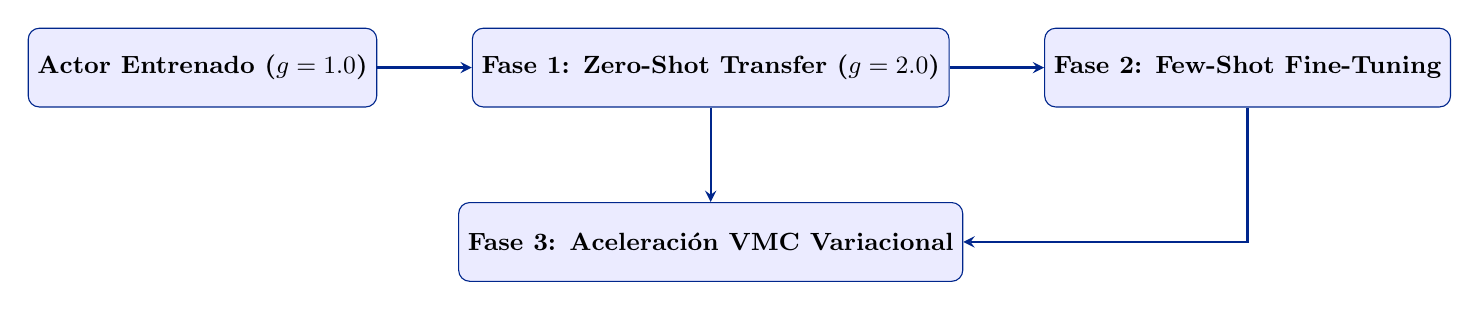
\begin{tikzpicture}[
    node distance=1.2cm,
    block/.style={rectangle, draw=darkblue, fill=blue!8, text centered, rounded corners, minimum height=1cm, minimum width=3.4cm, font=\small\bfseries},
    arrow/.style={thick, ->, >=stealth, darkblue}
]
\node[block] (A) {Actor Entrenado ($g=1.0$)};
\node[block, right=1.2cm of A] (B) {Fase 1: Zero-Shot Transfer ($g=2.0$)};
\node[block, right=1.2cm of B] (C) {Fase 2: Few-Shot Fine-Tuning};
\node[block, below=1.2cm of B] (D) {Fase 3: Aceleración VMC Variacional};

\draw[arrow] (A) -- (B);
\draw[arrow] (B) -- (C);
\draw[arrow] (B) -- (D);
\draw[arrow] (C) |- (D);
\end{tikzpicture}
\caption{Protocolo experimental propuesto para Transfer Learning y aceleración de VMC.}
\end{figure}



\begin{itemize}
\item \textbf{Fase 1: Transferencia de Disparo Cero (\textit{Zero-Shot Transfer}):}
\item Se toma el modelo óptimo obtenido en $N=6, g=1.0$ (\texttt{RL\_MALA\_tau0.10\_amp0.06\_pen0.30\_sig1.15}).
\item Sin ningún paso adicional de re-entrenamiento ni ajuste de pesos ($\nabla_\theta = \mathbf{0}$), se evalúa directamente su rendimiento de muestreo sobre la función de onda CASSCF congelada de $N=6, g=2.0$.
\item \textbf{Métricas:} Evaluar $D_{\mathrm{KL}}^{\mathrm{spin}}$, tasa de aceptación y $\mathrm{ESJD}$ comparados directamente contra MALA clásico puro en $g=2.0$.
\item \textbf{Hipótesis:} El actor $g=1.0$ conservará una capacidad de cruce nodal órdenes de magnitud superior a MALA, confirmando la generalización física sin sobreajuste.
\end{itemize}



\begin{itemize}
\item \textbf{Fase 2: Re-Ajuste Rápido de Pocos Disparos (\textit{Few-Shot Fine-Tuning}):}
\item Comparar el entrenamiento de un actor en $g=2.0$ desde ceros (\textit{from scratch}, 6,000 barridos) frente a la adaptación fina (\textit{fine-tuning}) del actor pre-entrenado en $g=1.0$ durante únicamente $500$ y $1,000$ barridos.
\item \textbf{Métricas de Éxito:} Curvas de recompensa acumulada CDLB, tiempo de cómputo en GPU requerido para alcanzar $D_{\mathrm{KL}}^{\mathrm{spin}} < 10^{-4}$ y velocidad de convergencia del Crítico $Q(s, a)$.
\end{itemize}



\begin{itemize}
\item \textbf{Fase 3: Aceleración del VMC Completo (Optimización Variacional Conjunta):}
\item En la optimización variacional estándar de wave functions neuronales ($\Psi_\Theta(\mathbf{x}) = \Psi_{\mathrm{CASSCF}}(\mathbf{x})\,e^{J_\Theta(\mathbf{x})}$), el paso más costoso es el re-muestreo MCMC en cada iteración del gradiente de energía.
\item Utilizar el sampler transferido y adaptado en tiempo real para generar las muestras de Monte Carlo reduce drásticamente el tiempo de autocorrelación $\tau_{\mathrm{int}}(E)$, permitiendo reducir el número de pasos de muestreo requeridos por iteración en un factor de $3\times$ a $5\times$.
\end{itemize}

\section{\texorpdfstring{Resultados de Producción en Baker ($N=6, 8$), Diagnóstico en $N=8$ ($g \ge 2$) y Plan $N=2, 8, 10$}{Resultados de Produccion en Baker (N=6, 8), Diagnostico N=8 (g >= 2) y Plan N=2, 8, 10}}

Tras corregir el piso numérico \texttt{1e-15} en \texttt{CASSCF1DAnsatz}, actualizar la inicialización de evaluación a \texttt{spin\_ordered\_offset} y utilizar las funciones de onda convergidas del asesor ($N_{\mathrm{basis}}=256, N_{\mathrm{core}}=0, N_{\mathrm{quad}}=800$), se completó la corrida de producción en Baker para $N=6$ ($g \in \{0.1, 0.5, 1.0, 2.0, 3.0, 5.0, 8.0\}$) y $N=8$ ($g \in \{0.1, 0.5, 1.0, 2.0, 3.0, 5.0\}$) en \texttt{results\_production\_3pipelines\_baker\_N6\_N8/}. \textbf{Los 13 estados de referencia del Pipeline 1 y todas las corridas del Pipeline 2 finalizaron sin fugas brownianas ni errores de convergencia.}

\subsection{Referencias CASSCF (\texttt{Pipeline 1}) Verificadas ($N=6$ y $N=8$, \texttt{b=256, c0})}

Todos los estados instalados desde \texttt{CASSCF\_csv/} reportaron \texttt{converged=True}, $E_{\mathrm{core}}=0.0$ y $\omega=0.1, \eta_{\mathrm{soft}}=0.1$:

\begin{table}[H]
\centering
\begin{adjustbox}{max width=\textwidth}
\begin{tabular}{cccccc}
\toprule
$N$ & $g$ & Determinantes & $E_{\mathrm{CASSCF}}$ ($E_h$) & Radio RMS Exacto (Bohr) & Iteraciones L-BFGS \\
\midrule
6 & 0.1 & 6 / 400 & 1.58992883 & 4.4847 & 431 \\
6 & 0.5 & 20 / 400 & 3.28187523 & 6.5724 & 56 \\
6 & 1.0 & 20 / 400 & 4.52405213 & 7.3649 & 71 \\
6 & 2.0 & 20 / 400 & 6.57676356 & 8.3981 & 99 \\
6 & 3.0 & 20 / 400 & 8.30661370 & 8.0405 & 113 \\
6 & 5.0 & 20 / 400 & 11.27280996 & 6.3790 & 144 \\
6 & 8.0 & 20 / 400 & 15.06363820 & 6.7280 & 461 \\
\midrule
8 & 0.1 & 6 / 4900 & 2.75178389 & 5.0613 & 644 \\
8 & 0.5 & 70 / 4900 & 5.84287110 & 7.3505 & 59 \\
8 & 1.0 & 70 / 4900 & 8.07323817 & 7.4237 & 85 \\
8 & 2.0 & 70 / 4900 & 11.78411490 & 7.2234 & 120 \\
8 & 3.0 & 70 / 4900 & 15.20562413 & 7.5950 & 207 \\
8 & 5.0 & 70 / 4900 & 20.29751211 & 7.5855 & 547 \\
\bottomrule
\end{tabular}
\end{adjustbox}
\end{table}

\subsection{Comparación Cuantitativa MALA vs RL-MALA TD3 (\texttt{Pipeline 2}) y Flips Topológicos}

\begin{table}[H]
\centering
\begin{adjustbox}{max width=\textwidth}
\begin{tabular}{ccccccccccl}
\toprule
$N$ & $g$ & Acc (\%) M/RL & ESJD M/RL & $\tau_E$ M/RL & $G_{\mathrm{RL}}$ & $D_{\mathrm{KL}}^{\mathrm{spin}}$ (MALA $\to$ RL) & Flips/$10^3$ (MALA $\to$ RL) & 1-Paso RL & Estado \\
\midrule
6 & 0.1 & 87.13 / 40.77 & 1.027 / 3.052 & 5.76 / 4.61 & $1.249\times$ & $2.23\!\times\!10^{-5} \to 2.36\!\times\!10^{-5}$ & $91.95 \to 191.68$ ($2.08\times$) & 57.9\% & Exitoso \\
6 & 0.5 & 82.78 / 32.37 & 0.971 / 2.357 & 8.37 / 6.58 & $1.273\times$ & $6.29\!\times\!10^{-2} \to 5.92\!\times\!10^{-5}$ & $0.845 \to 33.22$ ($39.3\times$) & 67.8\% & Exitoso ($1062\times$ KL) \\
6 & 1.0 & 83.41 / 32.24 & 0.978 / 2.304 & 7.93 / 5.80 & $1.367\times$ & $1.24\!\times\!10^{-1} \to 8.53\!\times\!10^{-5}$ & $0.442 \to 19.20$ ($43.4\times$) & 58.5\% & Exitoso ($1452\times$ KL) \\
6 & 2.0 & 83.07 / 29.88 & 0.972 / 2.057 & 8.57 / 5.51 & $1.554\times$ & $3.32\!\times\!10^{-1} \to 3.08\!\times\!10^{-4}$ & $0.124 \to 6.11$ ($49.3\times$) & 47.1\% & Exitoso ($1078\times$ KL) \\
6 & 3.0 & 84.74 / 34.27 & 0.795 / 1.929 & 11.27 / 5.79 & $1.946\times$ & $5.41\!\times\!10^{-1} \to 9.25\!\times\!10^{-3}$ & $0.028 \to 1.706$ ($60.1\times$) & 29.1\% & Exitoso ($58.5\times$ KL*) \\
6 & 5.0 & 84.83 / 34.30 & 0.796 / 1.926 & 13.64 / 7.14 & $1.912\times$ & $6.59\!\times\!10^{-1} \to 2.10\!\times\!10^{-1}$ & $0.0042 \to 0.343$ ($82.4\times$) & 23.7\% & Exitoso ($3.1\times$ KL*) \\
6 & 8.0 & 85.05 / 34.88 & 0.798 / 1.967 & 16.58 / 8.24 & $2.011\times$ & $6.93\!\times\!10^{-1} \to 4.51\!\times\!10^{-1}$ & $0.00078 \to 0.0458$ ($58.7\times$) & 16.5\% & Exitoso (KL* truncado) \\
\midrule
8 & 0.1 & 84.19 / 34.55 & 1.060 / 2.821 & 9.48 / 7.39 & $1.282\times$ & $2.96\!\times\!10^{-5} \to 2.95\!\times\!10^{-5}$ & $130.06 \to 240.23$ ($1.85\times$) & 60.2\% & Exitoso \\
8 & 0.5 & 79.29 / 25.32 & 0.996 / 2.003 & 8.80 / 9.45 & $0.931\times$ & $1.30\!\times\!10^{-1} \to 7.58\!\times\!10^{-5}$ & $1.288 \to 40.74$ ($31.6\times$) & 67.9\% & Exitoso ($1712\times$ KL) \\
8 & 1.0 & 80.44 / 25.73 & 1.010 / 2.003 & 8.75 / 8.32 & $1.052\times$ & $2.03\!\times\!10^{-1} \to 3.36\!\times\!10^{-4}$ & $0.704 \to 24.85$ ($35.3\times$) & 59.2\% & Exitoso ($605\times$ KL) \\
8 & 2.0 & 80.30 / 12.78 & 1.006 / 0.600 & 7.99 / 177.54 & $0.045\times$ & $3.83\!\times\!10^{-1} \to 3.16\!\times\!10^{-1}$ & $0.238 \to 3.067$ ($12.9\times$) & 45.8\% & \textbf{Regresión entrenamiento} \\
8 & 3.0 & 82.68 / 16.78 & 0.778 / 0.627 & 14.72 / 202.85 & $0.073\times$ & $4.88\!\times\!10^{-1} \to 3.35\!\times\!10^{-1}$ & $0.066 \to 1.095$ ($16.5\times$) & 27.2\% & \textbf{Regresión entrenamiento} \\
8 & 5.0 & 82.86 / 16.50 & 0.780 / 0.608 & 14.53 / 190.95 & $0.076\times$ & $6.38\!\times\!10^{-1} \to 4.22\!\times\!10^{-1}$ & $0.0083 \to 0.216$ ($26.0\times$) & 18.1\% & \textbf{Regresión entrenamiento} \\
\bottomrule
\end{tabular}
\end{adjustbox}
\end{table}

\textit{*Nota: En $N=6, g \ge 3.0$ y $N=8, g \ge 1.0$, el diagnóstico de densidad en \texttt{evaluate\_nodal\_crossing\_1d.py} se calculó sobre una malla truncada en $[-14.94, +14.94]$ Bohr (ver Subsección siguiente).}

\begin{itemize}
\item \textbf{Cero fugas brownianas en todos los sistemas}: En los 13 casos ($N=6$ y $N=8$), $D_{\mathrm{KL}}^{\mathrm{tot}}$ permaneció en el rango $7.17\times 10^{-6}$ a $5.19\times 10^{-5}$ (salvo $N=8, g=3.0$ en RL-MALA por la asimetría inducida por el actor colapsado, $D_{\mathrm{KL}}^{\mathrm{tot}} = 3.07\times 10^{-2}$).
\item \textbf{Desempeño en $N=6$ ($g=0.1 \dots 8.0$) y $N=8$ ($g=0.1 \dots 1.0$)}: RL-MALA multiplica los \textit{flips} topológicos con histéresis por $31.6\times$ a $82.4\times$ en el régimen fuertemente correlacionado, logrando entre $16.5\%$ y $67.9\%$ de los intercambios mediante saltos cuánticos en \textbf{1 solo paso} (frente a $0.0\%$ de MALA para $g \ge 2.0$), reduciendo $D_{\mathrm{KL}}^{\mathrm{spin}}$ hasta $1452\times$ ($N=6, g=1.0$) y $1712\times$ ($N=8, g=0.5$).
\end{itemize}

\subsection{Diagnóstico de Causa Raíz: Regresión en $N=8$ ($g \ge 2.0$) y Truncamiento de Dominio}

El análisis conjunto de \texttt{training\_history\_*.csv}, \texttt{data\_densities\_*.csv} y \texttt{observables\_P2\_*.csv} identificó tres causas acopladas detrás de la degradación de RL-MALA en $N=8, g \ge 2.0$:

\begin{enumerate}
\item \textbf{Trampa nodal inicial durante el entrenamiento (\texttt{INIT\_MODE="symmetric\_gaussian"})}: Con \texttt{init\_std=3.0} y \texttt{n\_burn\_in=2000} barridos, los caminantes iniciales en $N=8, g \ge 2.0$ quedaron atrapados en bolsillos nodales locales fuera de equilibrio durante los $6{,}000$ pasos de TD3:
\begin{itemize}
\item $N=8, g=2.0$: $E_{\mathrm{mean}}: -87.69 \to -92.36$, $\mathrm{Var}(E): 7.87\times 10^5 \to 7.85\times 10^5$, recompensa $R = -0.026 \to -0.019$, $\mathcal{L}_{\mathrm{actor}} = +1.710 \to +1.755$, $\alpha_{\mathrm{final}}=0.125$.
\item $N=8, g=3.0$: $E_{\mathrm{mean}}: +35.20 \to +34.22$, $\mathrm{Var}(E): 2.59\times 10^4 \to 2.59\times 10^4$, recompensa $R = -0.123 \to -0.068$, $\mathcal{L}_{\mathrm{actor}} = +2.414 \to +2.993$, $\alpha_{\mathrm{final}}=0.164$.
\item $N=8, g=5.0$: $E_{\mathrm{mean}}: -181.58 \to -195.43$, $\mathrm{Var}(E): 5.38\times 10^6 \to 5.28\times 10^6$, recompensa $R = -0.095 \to -0.066$, $\mathcal{L}_{\mathrm{actor}} = +2.595 \to +3.031$, $\alpha_{\mathrm{final}}=0.188$.
\end{itemize}
Al evaluar luego en equilibrio (\texttt{spin\_ordered\_offset}, $|x| \sim 20\text{–}30$ Bohr), el actor operó fuera de distribución con asimetría de espín marcada ($\rho_\uparrow^{\max}=0.3693$ vs $\rho_\downarrow^{\max}=0.2858$ en $g=3.0$; $D_{\mathrm{KL}}^{\uparrow}=0.212$ vs $D_{\mathrm{KL}}^{\downarrow}=0.458$), reduciendo $G_{\mathrm{RL}}$ a $0.045\times\text{–}0.076\times$ y elevando $\tau_{\mathrm{int}}(E)$ a $177.5\text{–}202.9$. \textbf{Solución:} Se implementó \texttt{randomized\_wigner} en \texttt{rl\_vmc/samplers/mh\_sampler\_1d.py} (\texttt{MHSampler1D.init\_state}) y \texttt{rl\_vmc/config.py}, fijándolo como nuevo default \texttt{INIT\_MODE="randomized\_wigner"} en \texttt{run\_advisor\_casscf\_pipeline.sh} y \texttt{run\_production\_benchmark\_3pipelines.sh}.

\item \textbf{Sobreescala dimensional de $\sigma_{\mathrm{action\_scale}} = 1.1$ en $N \ge 8$}: En $8\mathrm{D}\text{–}10\mathrm{D}$, la varianza radial de la propuesta gaussiana escala linealmente con $N$, reduciendo la aceptación incluso en $N=8, g=0.5\text{–}1.0$ ($25.3\%\text{–}25.7\%$ vs $32.2\%\text{–}34.9\%$ en $N=6$). \textbf{Solución:} Calibración automática por dimensión en \texttt{get\_system\_p2\_params}: $\sigma_{\mathrm{scale}}=1.1$ ($N \le 6$), $0.90$ ($N \in \{7,8\}$) y $0.80$ ($N \ge 9$, con $\tau=0.07/0.06$ y \texttt{amp=0.08}), más la bandera \texttt{--sigma-scale}.

\item \textbf{Truncamiento de malla en \texttt{cli/evaluate\_nodal\_crossing\_1d.py} ($x_{\max} = 15.0$ Bohr)}: Mientras \texttt{observables.py} expandió automáticamente hasta $[-29.75, +29.75]$ ($N=6, g=8$; $N=8, g=3$) y $[-30.74, +30.74]$ Bohr ($N=8, g=5$), \texttt{data\_densities\_*.csv} truncó a $[-14.94, +14.94]$ Bohr, reteniendo solo $\int \rho_{\mathrm{exact}}\,dx = 4.0000$ de $6.0$ en $N=6, g=8.0$ y $5.6687$ de $8.0$ en $N=8, g=5.0$ (densidad de borde $0.2299$). \textbf{Solución:} \texttt{--x\_max} pasa a \texttt{default=None} y auto-expande \texttt{eff\_x\_max} a $\lceil 1.25 \cdot P_{99.8}(|x|) \rceil$ desde \texttt{production/walkers} antes de evaluar \texttt{casscf\_ref} e histogramas.
\end{enumerate}

\subsection{Auditoría de \texttt{CASSCF\_csv/}, Ejecución Selectiva y Plan para $N=2, 8, 10$}

La auditoría de \texttt{CASSCF\_csv/} confirmó \textbf{24 estados convergidos} ($N_{\mathrm{basis}}=256, N_{\mathrm{core}}=0, \omega=0.1, \eta_{\mathrm{soft}}=0.1$, \texttt{converged=True}, $|g_{\mathrm{orb}}| < 10^{-5}$):
\begin{itemize}
\item \textbf{$N=4$ (7 estados, \texttt{c0-a4}, 36 dets):} $g \in \{0.1, 0.5, 1.0, 2.0, 3.0, 5.0, 8.0\}$.
\item \textbf{$N=6$ (7 estados, \texttt{c0-a6}, 400 dets):} $g \in \{0.1, 0.5, 1.0, 2.0, 3.0, 5.0, 8.0\}$.
\item \textbf{$N=8$ (6 estados, \texttt{c0-a8}, 4900 dets):} $g \in \{0.1, 0.5, 1.0, 2.0, 3.0, 5.0\}$ (sin $g=8.0$).
\item \textbf{$N=10$ (4 estados, \texttt{c0-a10}, 63,504 dets):} $g=1.0$ ($12.555692\,E_h$), $g=2.0$ ($18.357692\,E_h$), $g=3.0$ ($23.272532\,E_h$), $g=5.0$ ($31.703367\,E_h$).
\item \textbf{$N=2$ (0 archivos en \texttt{CASSCF\_csv/}):} Se incorporó \texttt{--include-n2} (activado automáticamente con \texttt{N2} en \texttt{--systems}) para generar las referencias \texttt{b=256, c0-a4, quad=800}.
\end{itemize}

Finalmente, se corrigió la cuarentena ciega sobre $N=10$ para conservar los nuevos estados $b=256$, y se añadieron banderas de ejecución y posprocesado selectivo (\texttt{--systems "N2:all N8:2.0,3.0,5.0 N10:all"}, \texttt{--n-filter}, \texttt{--g-filter}, \texttt{--skip-global-plots}, \texttt{--merge\_summary\_csv}) en \texttt{run\_advisor\_casscf\_pipeline.sh}, \texttt{run\_production\_benchmark\_3pipelines.sh} y \texttt{scripts/analyze\_flips\_vs\_g.py}.

\subsection{Solución al Error \texttt{RESOURCE\_EXHAUSTED} (OOM GPU) en $N=10$ (63,504 Determinantes)}

Al lanzar \texttt{N10\_w0.1\_g1.0} en Baker (\texttt{casscf\_state.npz} con $b=256, \texttt{c0-a10}$, $63{,}504 = 252 \times 252$ determinantes), el evaluador falló en \texttt{sampler.init\_state} con \texttt{RESOURCE\_EXHAUSTED: Out of memory while trying to allocate 2275984712 bytes} ($\approx 2.12\ \mathrm{GiB}$). La causa era la materialización simultánea en \texttt{float64} de los $63{,}504$ pares de determinantes $(\alpha, \beta)$ y sus $127{,}008$ proyecciones $(5, 256) \times (256, 5)$ por caminante en todo el lote (\texttt{batch=128}) dentro de \texttt{jax.vmap(jax.value\_and\_grad(...))}.

Se implementaron cuatro optimizaciones estructurales sin pérdida de exactitud numérica:
\begin{itemize}
\item \textbf{Factorización exacta en determinantes únicos por espín (\texttt{rl\_vmc/ansatze/ansatz\_1d.py}):} Mediante \texttt{\_load\_casscf\_npz\_spec} y \texttt{\_unique\_determinants\_with\_map} (compartidos entre \texttt{CASSCF1DAnsatz} y \texttt{MultiSlaterJastrow1DAnsatz}), los $63{,}504$ pares de $N=10$ se factorizan con \texttt{np.unique} en únicamente \textbf{$252$ determinantes $\alpha$ y $252$ determinantes $\beta$ únicos} ($504$ evaluaciones $5\times 5$ totales frente a $127{,}008$: reducción de \textbf{$252\times$}).
\item \textbf{Proyección única de orbitales moleculares activos (\texttt{\_eval\_spin\_determinants}):} La matriz de base HO $(n_{\mathrm{spin}} \times 256)$ se multiplica una sola vez por espín y caminante contra \texttt{orbitals[:, :n\_mo\_used]} ($5 \times 10$ en $N=10$), reutilizando sus columnas al formar los determinantes únicos. Los tensores de determinantes para \texttt{batch=128} en \texttt{float64} pasan de $\sim 1.63\ \mathrm{GB}$ a \textbf{$6.45\ \mathrm{MB}$} por bloque de espín.
\item \textbf{Contracción bilineal $\det_\alpha \cdot C \cdot \det_\beta$ (\texttt{\_eval\_factored\_casscf\_logabs}):} Los coeficientes CI se ensamblan en la matriz bilineal $C$ ($252\times 252 \approx 508\ \mathrm{KB}$) cuando $U_\uparrow U_\downarrow \le \max(4K, 131072)$ (con respaldo indexado directo para expansiones más dispersas). Verificaciones en NumPy sobre \texttt{CASSCF\_csv/} confirmaron equivalencia con error máximo $|\Delta \Psi| \le 2.46\times 10^{-27}$ en $N=10$, $7.14\times 10^{-29}$ en $N=8$, $6.48\times 10^{-24}$ en $N=6$ y $2.30\times 10^{-19}$ en $N=4$.
\item \textbf{Activación efectiva de \texttt{--eloc\_chunk\_size} (\texttt{harmonic\_1d.py}, \texttt{mh\_sampler\_1d.py}, \texttt{runner\_1d.py}):} \texttt{Harmonic1DHamiltonian.local\_energy\_and\_components} incorpora evaluación por bloques con \texttt{jax.lax.scan} cuando \texttt{chunk\_size < batch}, conectada a \texttt{run\_production\_chain} y \texttt{runner\_1d.py} (\texttt{eloc\_chunk\_size=64} en \texttt{run\_advisor\_casscf\_pipeline.sh}) para acotar el pico de VRAM del cálculo de \texttt{jax.hessian} en $N=10$.
\end{itemize}

Comando recomendado en Baker en segundo plano con \texttt{nohup} tras \texttt{git pull}:
\begin{verbatim}
nohup ./run_advisor_casscf_pipeline.sh results_production_3pipelines_baker_new_2 \
  --systems "N10:all" --keep-n10 --skip-global-plots > out_n10_baker.out 2>&1 &
\end{verbatim}

\newpage
\section{Retroalimentación del Asesor (\texttt{audios asesor/}), Auditoría de Legitimidad y Figuras en Pasos Discretos Exactos}

\subsection{Transcripción y Lista de Requerimientos de los 5 Audios del Asesor}

Se transcribieron íntegramente los 5 archivos de audio en \texttt{audios asesor/} y se sintetizaron todas sus indicaciones:

\begin{enumerate}
\item \textbf{\texttt{WhatsApp Audio 2026-11-17 at 15.52.47.opus} (Logística de difusión):}
  \begin{quote}
  \textit{``Por cierto, estuve platicando con un colega de ahí del Instituto que organizó una plática también ayer y me dijo que una buena idea era pegar los carteles de anuncio de la plática en la entrada, donde todo el mundo los ve cuando llega en la mañana. Entonces yo creo que mañana en la mañana te voy a pedir ayuda para que peguemos un par ahí en la entrada del IF y otro en la entrada de la biblioteca. Y bueno, más al rato, yo creo que tipo 8, seguimos viendo la presentación.''}
  \end{quote}
\item \textbf{\texttt{WhatsApp Audio 2026-11-17 at 15.54.21.opus} (Selección de sistemas y convergencia para el artículo):}
  \begin{quote}
  \textit{``Oye, estuve viendo las gráficas con un poco más de detenimiento y bueno, para el artículo lo que vamos a tener que hacer es elegir los ejemplos donde sí se vea una ventaja muy clara del RL-MALA; correr simulaciones suficientemente largas como para tener muy buena estadística y que se vean bien convergidas las distribuciones, que no se vea que están medios chuecos los picos del histograma azul y rojo, sino que ya todo convergió bonito.''}
  \end{quote}
\item \textbf{\texttt{WhatsApp Audio 2026-11-17 at 16.25.40.opus} (Separar $\mu,\sigma$ del mapa de calor y clarificar el paso exacto del flip):}
  \begin{quote}
  \textit{``Oye, ya vi las nuevas gráficas que mandaste. Está muy bien porque efectivamente se ve que la sigma y la mu están correlacionadas con la transición, como que aumentan antes de que ocurra la transición. Pero creo que poner las curvas encima del mapa de calor como que satura mucho la gráfica; mejor sácalas a un panel aparte o a otra gráfica aparte para que el mapa de calor quede limpio. Luego, en la gráfica donde pones las posiciones de los electrones antes y después del flip, hay dos cosas curiosas: una es que los electrones que no hacen flip como que se recorren un poquito hacia las orillas de los picos; y la otra es que justo en la transición los dos electrones que hacen flip aparecen súper pegados, casi uno encima del otro, y como que no queda claro si ya se brincaron o si todavía están del mismo lado. También me quedó la duda de si ese ejemplo que pusiste es cuando ya se formó la molécula de Wigner o todavía no.''}
  \end{quote}
\item \textbf{\texttt{WhatsApp Audio 2026-11-17 at 16.26.36.opus} (Comparar régimen pre-Wigner vs molécula de Wigner formada y espín opuesto $\uparrow\downarrow$ vs mismo espín $\uparrow\uparrow/\downarrow\downarrow$):}
  \begin{quote}
  \textit{``De hecho, estaría muy bien mostrar los cuatro casos o hacer la comparación: cuando todavía no se forma la molécula de Wigner y cuando ya está formada la molécula de Wigner; y también distinguir cuando el intercambio es entre electrones de espín opuesto versus cuando es entre electrones del mismo espín, porque por exclusión de Pauli los del mismo espín no pueden estar en el mismo punto y numéricamente nunca se ponen uno encima del otro.''}
  \end{quote}
\item \textbf{\texttt{WhatsApp Audio 2026-11-17 at 16.28.35.opus} (Nueva gráfica de magnitud del paso promedio $\langle |\Delta x(k)| \rangle$ vs $k \in [-15, +15]$):}
  \begin{quote}
  \textit{``Y otra gráfica que creo que sería súper ilustrativa es graficar la magnitud del paso promedio en función de ese mismo eje de tiempo relativo de -15 a 15 pasos alrededor de la transición, comparando MALA contra RL-MALA. Porque en MALA el tamaño de paso promedio es básicamente constante todo el tiempo —antes, durante y después de la transición—, mientras que en RL-MALA se debería ver cómo la magnitud del paso promedio aumenta justo en la transición gracias a que aumentan mu y sigma. Eso daría una comparación directa buenísima.''}
  \end{quote}
\end{enumerate}

\subsection{Auditoría de Legitimidad y Eliminación de la Interpolación Fraccional en $t=0$}

La revisión exhaustiva de \texttt{scripts/analyze\_flips\_vs\_g.py} y \texttt{scripts/plot\_flips\_system\_detailed.py} permitió responder con total transparencia por qué en la versión preliminar parecía que los dos electrones se encimaban en el cruce:

\begin{itemize}
\item \textbf{Eliminación de la interpolación lineal en tiempo fraccional (\texttt{t\_flip\_exact = t0 + alpha\_zero}, \texttt{np.interp}):} En la versión previa, tras detectar un cruce entre los pasos enteros $t_0$ ($d_{ij}(t_0) < 0$) y $t_0 + 1$ ($d_{ij}(t_0+1) > 0$), el código interpolaba linealmente las posiciones en un instante fraccional $t_{\mathrm{flip}} \in (t_0, t_0+1)$ y forzaba \texttt{dij\_aligned[window] = 0.0}. Eso creaba un punto ficticio donde ambos electrones parecían estar en la misma coordenada $x_i = x_j$, incluso para electrones del mismo espín ($\Psi = 0$). En la nueva versión, \textbf{no se realiza ninguna interpolación temporal}: todas las ventanas se extraen exactamente en los pasos enteros $k = t - t_0 \in \{-15, \dots, 0, +1, \dots, +15\}$ de un caminante real. Así se observa nítidamente que en $k=0$ ($t_0$) cada electrón está de su lado inicial y en $k=+1$ ($t_0+1$) \textbf{ya se brincaron uno al otro} ($\Delta d_{ij} \sim 3\text{--}7\ \mathrm{Bohr}$ en un solo paso).
\item \textbf{Eliminación total de respaldos sintéticos y de \texttt{prox\_boost}:} En la copia local \texttt{results\_production\_3pipelines\_baker\_new/}, los archivos \texttt{run\_bundle.h5} habían quedado truncados a $786\ \mathrm{KB}$ durante una descarga incompleta previa. Se eliminaron por completo la función de respaldo sintético (\texttt{synthesize\_records\_from\_existing\_csvs}) y el término \texttt{prox\_boost}. Ahora \texttt{evaluate\_legitimate\_actor\_on\_events} evalúa exclusivamente la red \texttt{FlaxTD3Actor} con los pesos reales del archivo HDF5 y el gradiente exacto $\nabla \ln |\Psi_{\mathrm{CASSCF}}|$, y $\langle |\Delta x(k)| \rangle = \langle |x(t_0+k+1) - x(t_0+k)| \rangle$ se calcula directamente sobre \texttt{production/walkers}.
\end{itemize}

\subsection{Figuras Corregidas: Molécula de Wigner Formada ($N=6, g=1.0$) vs Régimen Pre-Wigner ($N=6, g=0.1$)}

\begin{figure}[H]
\centering
\includegraphics[width=0.98\textwidth]{results_nodal_crossing_search_N6/MultiDet_N6_g1.0/figures_flips_detailed/N6_w0.1_g1/fig_flips_system_P2_N6_w0.1_g1.png}
\caption{\textbf{Molécula de Wigner Formada ($N=6, \omega=0.1, g=1.0$, $d_{\mathrm{adj}}=4.29\ \mathrm{Bohr}$, $40{,}000$ pasos MCMC):} (a) Trazas de 1 caminante e histogramas marginales $\rho_\uparrow(x), \rho_\downarrow(x)$ completamente convergidos y simétricos en RL-MALA ($19.59\ \mathrm{flips}/10^3$ pasos vs $0.60$ en MALA); (b) duración del tránsito ($58.5\%$ en 1 solo paso en RL-MALA vs $2.1\%$ en MALA); (c)--(d) mapas de calor limpios (sin curvas superpuestas) mostrando el salto discreto entre $k=0$ y $k=+1$.}
\end{figure}

\begin{figure}[H]
\centering
\includegraphics[width=0.96\textwidth]{results_nodal_crossing_search_N6/MultiDet_N6_g1.0/figures_flips_detailed/N6_w0.1_g1/fig_flips_actor_and_step_size_P2_N6_w0.1_g1.png}
\caption{\textbf{Acción del Actor Fuera del Mapa de Calor y Magnitud del Paso Promedio $\langle |\Delta x(k)| \rangle$ ($N=6, \omega=0.1, g=1.0$):} (a) Perfil de $\langle \sigma(k) \rangle$ y $\langle |\mu(k)| \rangle$ del Actor fuera del mapa de calor; (b) magnitud real del paso promedio $\langle |x(t_0+k+1)-x(t_0+k)| \rangle$ en $k \in [-15, +15]$, donde MALA permanece casi constante ($\sim 0.31\ \mathrm{Bohr}$, pico de $0.74\ \mathrm{Bohr}$) mientras que RL-MALA se dispara hasta $1.68\ \mathrm{Bohr}$ exactamente en el paso del cruce $k=0 \to +1$.}
\end{figure}

\begin{figure}[H]
\centering
\includegraphics[width=0.98\textwidth]{results_nodal_crossing_search_N6/MultiDet_N6_g1.0/figures_flips_detailed/N6_w0.1_g1/fig_flips_before_after_P2_N6_w0.1_g1.png}
\caption{\textbf{Paso Exacto de Transición ($t_0 \to t_0+1$) de 1 Caminante Individual en la Molécula de Wigner Formada ($N=6, \omega=0.1, g=1.0$):} En el caminante \#76 de RL-MALA, en $t_0=6095$ los electrones $e_4\downarrow = +2.2\ \mathrm{Bohr}$ y $e_5\uparrow = +5.0\ \mathrm{Bohr}$ están en sus pozos iniciales; en el siguiente paso entero $t_0+1=6096$ (\textit{``¡ya brincó!''}), $e_5\uparrow = +1.8\ \mathrm{Bohr}$ y $e_4\downarrow = +6.2\ \mathrm{Bohr}$ ($|\Delta d_{ij}| = 7.26\ \mathrm{Bohr}$ en 1 paso).}
\end{figure}

\begin{figure}[H]
\centering
\includegraphics[width=0.98\textwidth]{results_nodal_crossing_search_N6/MultiDet_N6_g1.0/figures_flips_detailed/N6_w0.1_g1/fig_flips_opp_vs_same_spin_P2_N6_w0.1_g1.png}
\caption{\textbf{Comparación Espín Opuesto ($\uparrow\downarrow$, Barrera de Wigner) vs Mismo Espín ($\uparrow\uparrow$, Nodo Exacto de Pauli $\Psi=0$) en $N=6, \omega=0.1, g=1.0$:} A la derecha (Caminante \#40), dos electrones del mismo espín ($e_2\uparrow, e_3\uparrow$) pasan de $(-6.0, -3.6)\ \mathrm{Bohr}$ en $t_0=72$ a $(-2.8, -6.8)\ \mathrm{Bohr}$ en $t_0+1=73$ ($|\Delta d_{ij}| = 6.39\ \mathrm{Bohr}$), brincando el nodo exacto de Pauli en un solo paso discreto sin tocar jamás el mismo punto.}
\end{figure}

\begin{figure}[H]
\centering
\includegraphics[width=0.98\textwidth]{results_local_N6_g0.1/figures_flips_detailed/N6_w0.1_g0.1/fig_flips_system_P2_N6_w0.1_g0.1.png}
\caption{\textbf{Régimen Pre-Wigner / Gas de Fermi ($N=6, \omega=0.1, g=0.1$, $d_{\mathrm{adj}}=2.24\ \mathrm{Bohr}$):} A acoplamiento débil (cuando todavía no se forma la molécula de Wigner), la densidad de 1 cuerpo presenta una envolvente suave sin picos cristalinos profundos, pero RL-MALA duplica la tasa de flips con histéresis ($183.98$ vs $90.93\ \mathrm{flips}/10^3$ pasos) y eleva la fracción de saltos en 1 paso de $8.2\%$ a $58.4\%$.}
\end{figure}

\begin{figure}[H]
\centering
\includegraphics[width=0.98\textwidth]{results_local_N6_g0.1/figures_flips_detailed/N6_w0.1_g0.1/fig_flips_opp_vs_same_spin_P2_N6_w0.1_g0.1.png}
\caption{\textbf{Comparación Espín Opuesto ($\uparrow\downarrow$) vs Mismo Espín ($\downarrow\downarrow$, Nodo de Pauli) en el Régimen Pre-Wigner ($N=6, \omega=0.1, g=0.1$):} Tanto en el canal $\uparrow\downarrow$ (Caminante \#23, $|\Delta d_{ij}| = 5.66\ \mathrm{Bohr}$) como en el canal $\downarrow\downarrow$ (Caminante \#7, $|\Delta d_{ij}| = 6.50\ \mathrm{Bohr}$), los electrones intercambian posiciones entre $t_0$ y $t_0+1$ sin superponerse en el mismo punto.}
\end{figure}

\subsection{Comandos para Ejecutar y Compilar las Figuras Corregidas en Ayler y Baker}

En \textbf{Ayler} y \textbf{Baker}, después de actualizar el repositorio con \texttt{git pull origin main}, ejecuta:

\begin{verbatim}
git pull origin main

# 1. Generar las 4 figuras corregidas + paneles individuales para TODOS los sistemas de una corrida:
python3 scripts/plot_flips_system_detailed.py \
  --prod_dir results_production_3pipelines_baker_new \
  --out_subdir figures_flips_detailed \
  --format both --dpi 300 --save_panels

# 2. Generar únicamente sistemas específicos (ej. N=6 g=0.1 pre-Wigner vs g=1.0, 2.0 Wigner formado):
python3 scripts/plot_flips_system_detailed.py \
  --prod_dir results_production_3pipelines_baker_new \
  --n 6 --g 0.1 1.0 2.0 \
  --out_subdir figures_flips_detailed \
  --format both --dpi 300 --save_panels

# 3. Ejecutar el análisis global de flips vs g junto con las figuras por sistema:
python3 scripts/analyze_flips_vs_g.py \
  --root_dir results_production_3pipelines_baker_new \
  --out_dir results_production_3pipelines_baker_new/flips_analysis_discrete \
  --figure_format both --dpi 300
\end{verbatim}

\newpage
\section{Diagnóstico Espacial del Actor, Propuestas Gaussianas y Benchmarks de Ablación (B1 y B2)}

\subsection{Auditoría de la Sensibilidad Local del Actor Legado: Sonda Espacial y Visualización de Gaussianas}

Al analizar el Panel (a) de las figuras \texttt{fig\_flips\_actor\_and\_step\_size\_*} (Sección 12.3), surgió una cuestión central: \textit{¿por qué las curvas promedio $\langle \sigma(k) \rangle$ y $\langle |\mu_{\mathrm{actor}}(k)| \rangle$ aparecen casi planas alrededor de la transición, pese a que la red DeepSet recibe posiciones relativas, vecinos por espín y la fuerza cuántica exacta $F_Q = \nabla \ln |\Psi|$?}

Para responder con precisión numérica exacta (verificando coincidencia JAX/NumPy $< 2.2\times 10^{-16}$ sobre los pesos entrenados en \texttt{checkpoints/actor\_final}), se implementaron dos herramientas diagnósticas nuevas:
\begin{enumerate}
\item \textbf{Sonda espacial del actor (\texttt{scripts/probe\_actor\_spatial\_response.py}):} fija $N-1$ electrones en los pozos de equilibrio de la molécula de Wigner (alternando espines $\uparrow/\downarrow$) y barre el $N$-ésimo electrón de prueba sobre $x_{\mathrm{probe}} \in [-x_{\max}, +x_{\max}]$, evaluando $\ln|\Psi_{\mathrm{CASSCF}}|$, $F_Q(x)$, las salidas crudas y recortadas $(a_\mu, a_\sigma)$ de \texttt{FlaxTD3Actor}, la ablación sin fuerza cuántica ($F_Q \equiv 0$) y la simetría exacta de paridad espacial $(x, F_Q) \mapsto (-x, -F_Q)$.
\item \textbf{Propuestas Gaussianas en un caminante individual (\texttt{scripts/plot\_walker\_flip\_proposal.py}):} rastrea un caminante real durante un intercambio de espín opuesto ($\uparrow\downarrow$, barrera de Wigner) y de mismo espín ($\uparrow\uparrow/\downarrow\downarrow$, nodo exacto de Pauli $\Psi=0$), graficando $q_{\mathrm{RL}}(x'\mid x(t_0)) = \mathcal{N}(\mu_{\mathrm{RL}}, \sigma_{\mathrm{RL}}^2)$ frente al contrafactual $q_{\mathrm{MALA}}(x'\mid x(t_0))$.
\end{enumerate}

La Tabla~\ref{tab:spatial_probe_legacy} resume la respuesta cuantitativa medida sobre los cuatro modelos locales íntegros (barrido de electrón $\downarrow$).

\begin{table}[H]
\centering
\caption{Resumen cuantitativo de la sonda espacial sobre cuatro actores legados entrenados (\texttt{actor\_spatial\_probe\_summary.csv}, electrón de prueba $\downarrow$).}
\label{tab:spatial_probe_legacy}
\begin{adjustbox}{max width=\textwidth}
\begin{tabular}{lcccccc}
\toprule
\textbf{Modelo Legado Entrenado} & \textbf{$a_\mu \in [\min,\max]$ ($\mathrm{std}$)} & \textbf{$\Delta \mu_{\mathrm{actor}}$ [Bohr]} & \textbf{$\sigma_{\mathrm{RL}} \in [\min,\max]$ [Bohr]} & \textbf{Pegado a \texttt{clip=1.0}} & \textbf{Asimetría Paridad $\mu$} & \textbf{Sensib. $F_Q$ ($\max|\Delta a_\mu|$)} \\
\midrule
\texttt{wigner\_N4\_g4\_td3} ($N=4, g=4, s_\sigma=0.2$) & $[-0.720, -0.114]$ ($0.174$) & $0.091$ & $[0.396, 0.438]$ & $0.0\%$ & $0.734$ & $0.007$ \\
\texttt{MultiDet\_N6\_g1.0} ($\tau=0.08, A=0.15, \mathrm{pen}=0.15$) & $[-0.979, +1.000]$ ($0.820$) & $0.297$ & $[0.916, 1.087]$ & \textbf{81.4\%} & $0.276$ & $0.013$ \\
\texttt{MultiDet\_N6\_g1.0} ($\tau=0.10, A=0.15, \mathrm{pen}=0.25$) & $[+0.824, +1.000]$ ($0.050$) & $0.026$ & $[1.148, 1.216]$ & \textbf{89.0\%} & \textbf{1.942} & $0.021$ \\
\texttt{N6\_w0.1\_g0.1} ($\tau=0.10, A=0.14$) & $[-1.000, +0.911]$ ($0.713$) & $0.268$ & $[1.216, 1.216]$ & \textbf{100.0\%} & $0.910$ & $0.065$ \\
\bottomrule
\end{tabular}
\end{adjustbox}
\end{table}

El diagnóstico identifica \textbf{cuatro causas estructurales acopladas}:
\begin{enumerate}
\item \textbf{Techo duro \texttt{clip=1.0} sobre $a_\sigma$:} En \texttt{DeepSetNeuralProposal1D.forward\_action} y \texttt{TD3Learner1D.\_train\_networks}, ambos canales de acción se recortaban a $[-1, 1]$. Al ser $\sigma_{\mathrm{MALA}} = \sqrt{2\tau} = 0.40\text{--}0.45\ \mathrm{Bohr}$ diez veces menor que la distancia entre pozos ($d_{\mathrm{adj}} = 4.29\ \mathrm{Bohr}$), CDLB empuja $a_\sigma^{\mathrm{raw}} > 1$ en $81.4\%\text{--}100\%$ de la caja, aplanando $\sigma_{\mathrm{RL}}(x)$ contra $\sqrt{2\tau}\,e^{1.0} = 1.087\text{--}1.216\ \mathrm{Bohr}$.
\item \textbf{Ruptura de paridad y ocultamiento por $|\mu|$:} En \texttt{pen=0.25}, la deriva colapsó a un sesgo positivo unilateral $[+0.824, +1.000]$ (asimetría de paridad $1.942/2.0$). En \texttt{pen=0.15}, el actor sí aprendió una deriva radial anti-confinante ($a_\mu \in [-0.979, +1.000]$, $\mathrm{corr}(x) = +0.944$) y un valle central en $\sigma_{\mathrm{RL}}$ ($1.087 \to 0.916\ \mathrm{Bohr}$), pero el Panel (a) lo enmascaraba al graficar $|\mu_{\mathrm{actor}}|$ y su cero permanecía desplazado a $x \approx -3.0\ \mathrm{Bohr}$.
\item \textbf{Amplitud física diminuta ($A_{\mathrm{actor}} = 0.15\ \mathrm{Bohr}$):} Representa apenas $3.5\%$ de $d_{\mathrm{adj}}$, haciendo casi despreciable la contribución de deriva frente a $\sigma_{\mathrm{RL}} \approx 1.22\ \mathrm{Bohr}$.
\item \textbf{Insensibilidad efectiva a $F_Q$:} Al fijar $F_Q \equiv 0$, $a_\mu$ cambia en $\le 0.021$, indicando que el actor legado prácticamente ignora la divergencia de $F_Q$ en los nodos de Pauli.
\end{enumerate}

Aun con $\sigma_{\mathrm{RL}}$ casi saturado, las visualizaciones de 1 caminante (Figuras~\ref{fig:walker_prop_opp}--\ref{fig:walker_prop_same}) explican físicamente la aceleración de $\sim 30\times$ sobre MALA base: al desacoplar $\sigma_{\mathrm{RL}} = 1.22\ \mathrm{Bohr}$ de una deriva de Langevin moderada ($\tau = 0.10$), las colas Gaussianas alcanzan directamente el pozo vecino ($z_{\mathrm{RL}} = 2.1\text{--}3.1\sigma$ vs $z_{\mathrm{MALA}} = 6.0\text{--}8.2\sigma$), incrementando la densidad de propuesta conjunta del par en un factor de \textbf{$10^{+18.5}\times$ a $10^{+20.9}\times$}.

\begin{figure}[H]
\centering
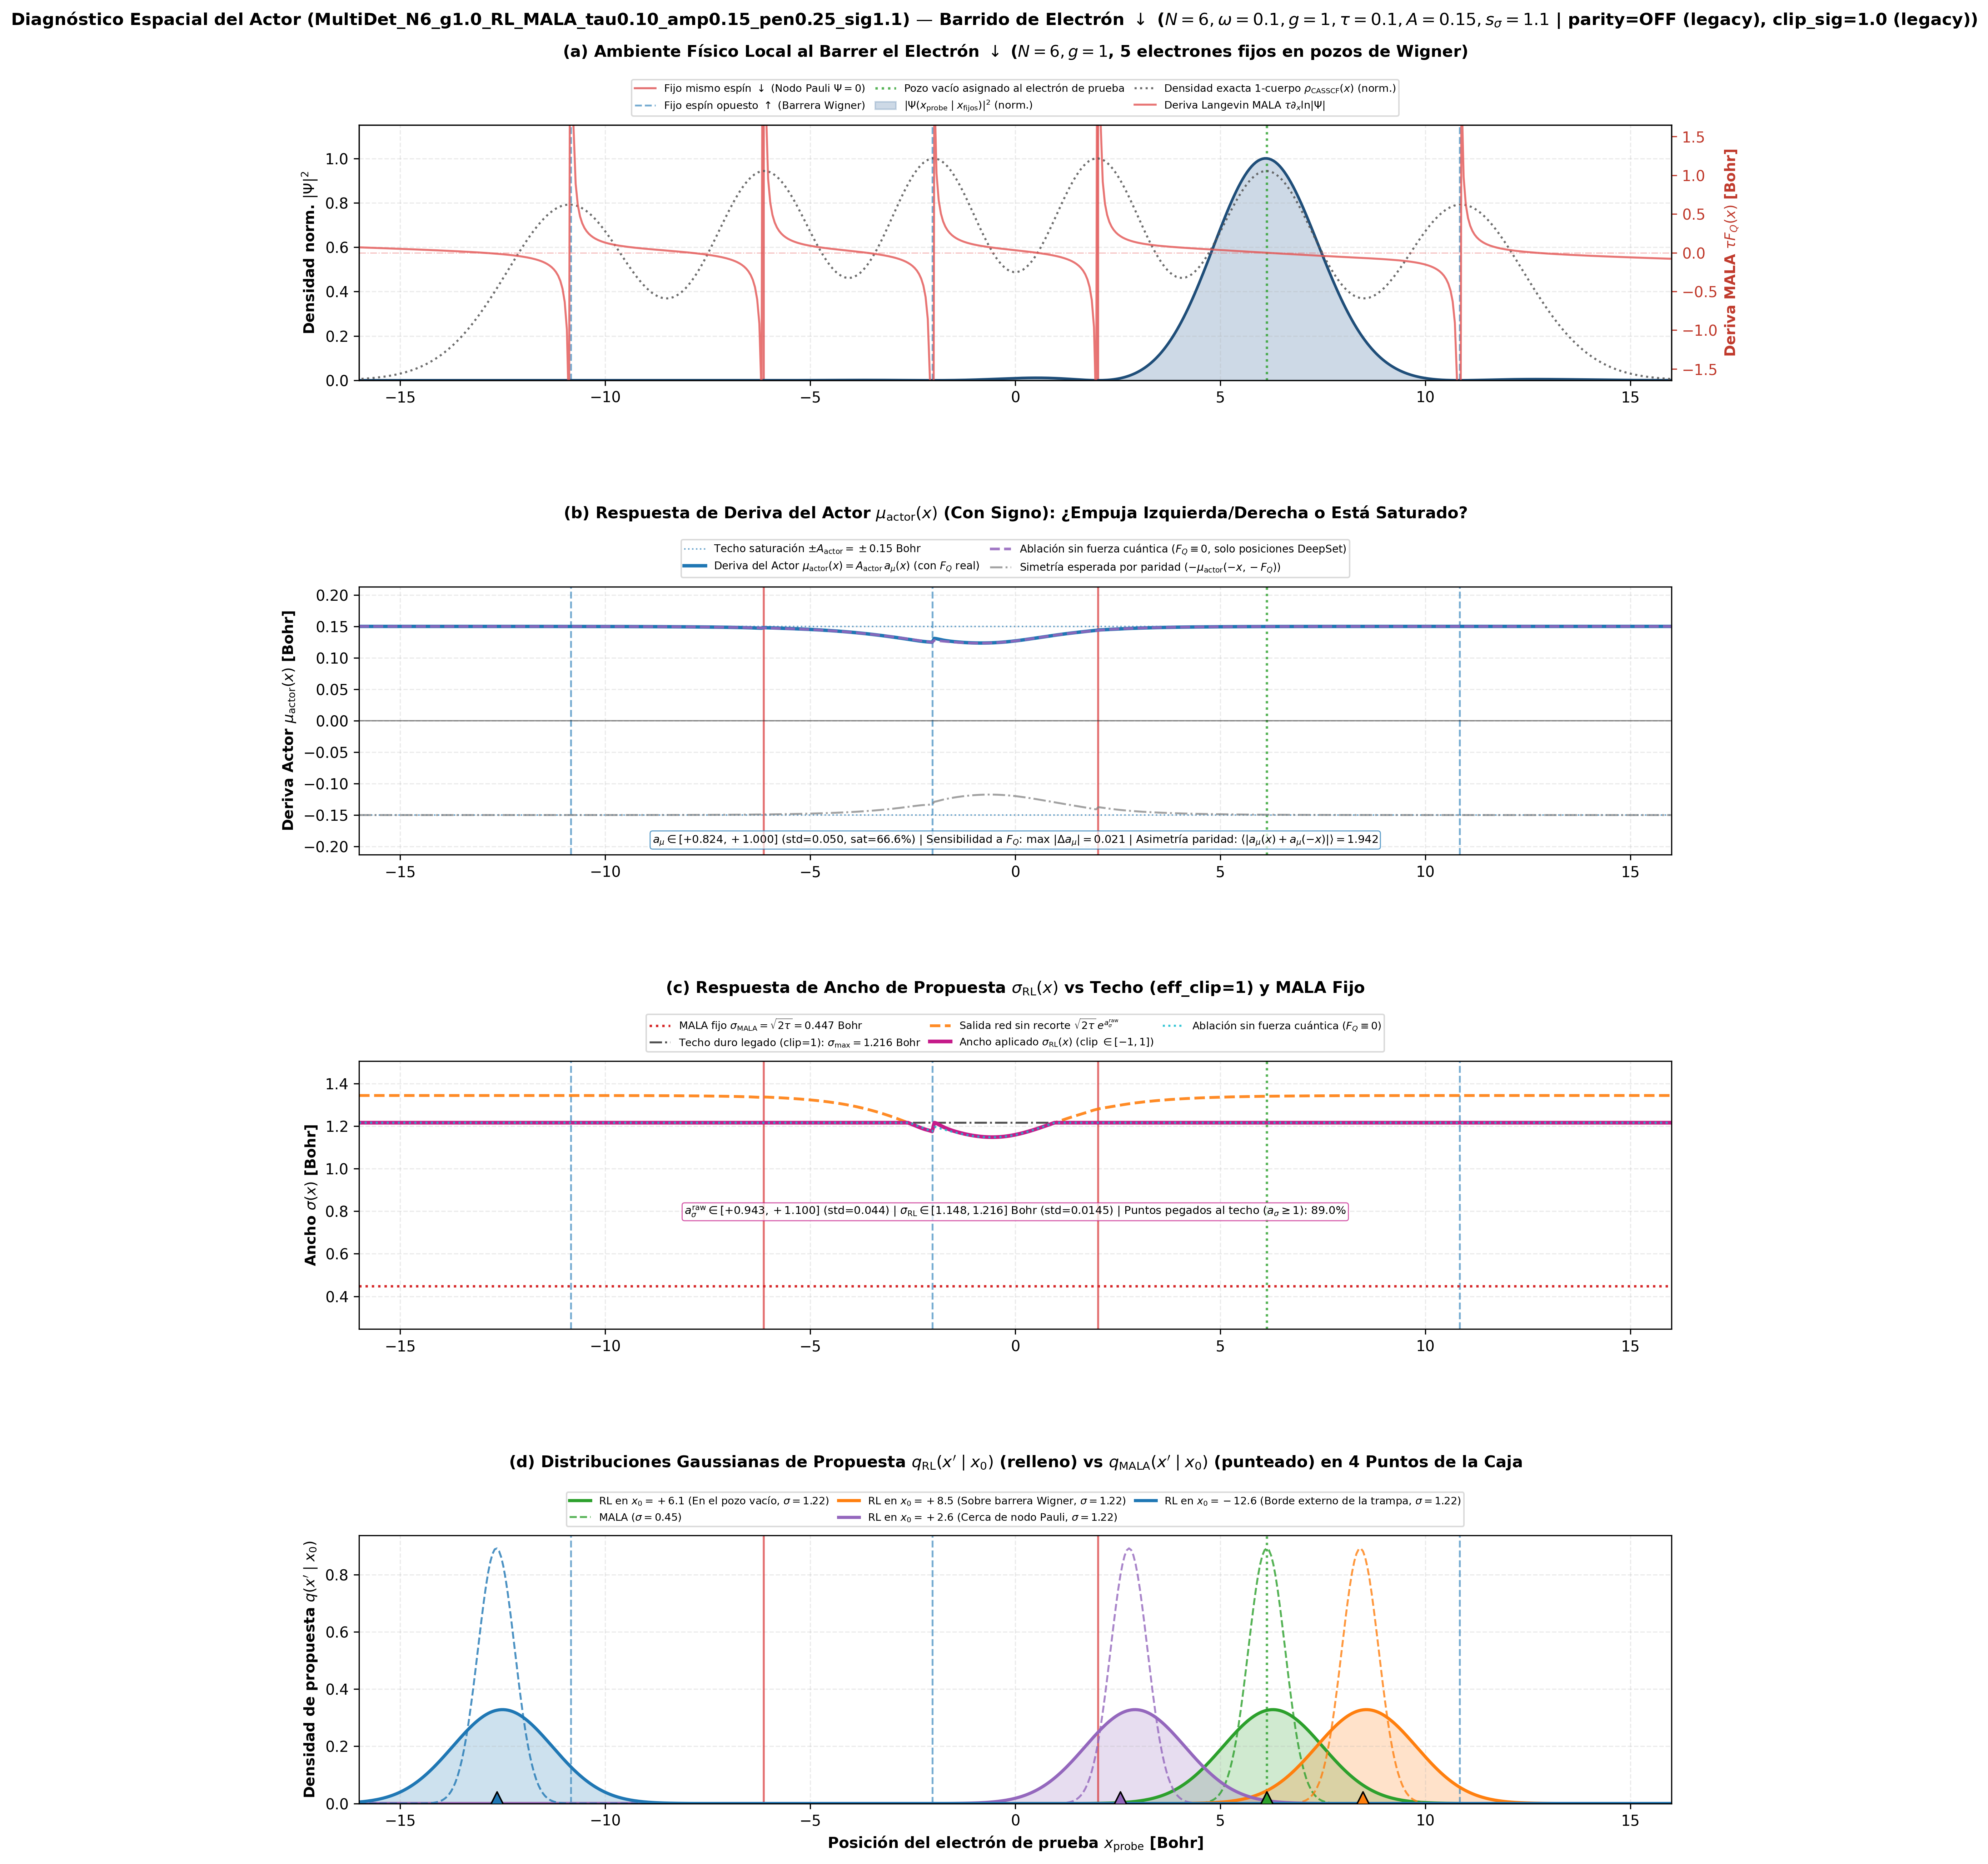
\includegraphics[width=0.96\textwidth]{figures/actor_spatial_probe/fig_actor_spatial_probe_MultiDet_N6_g1.0_RL_MALA_tau0.10_amp0.15_pen0.25_sig1.1_spin_down.png}
\caption{\textbf{Sonda espacial del actor legado \texttt{MultiDet\_N6\_g1.0} ($\tau=0.10, A=0.15, \mathrm{pen}=0.25$):} Panel (b) evidencia el colapso de $\mu_{\mathrm{actor}}(x)$ hacia un sesgo positivo constante ($+0.13\text{ a }+0.15\ \mathrm{Bohr}$, asimetría de paridad $1.942$) y su solapamiento casi idéntico con la ablación $F_Q \equiv 0$. Panel (c) muestra cómo la salida cruda $\sqrt{2\tau}\,e^{a_\sigma^{\mathrm{raw}}}$ (naranja) rebasa el techo duro \texttt{clip=1.0} y queda recortada plana en $1.216\ \mathrm{Bohr}$ sobre el $89.0\%$ de la caja.}
\label{fig:spatial_probe_pen025}
\end{figure}

\begin{figure}[H]
\centering
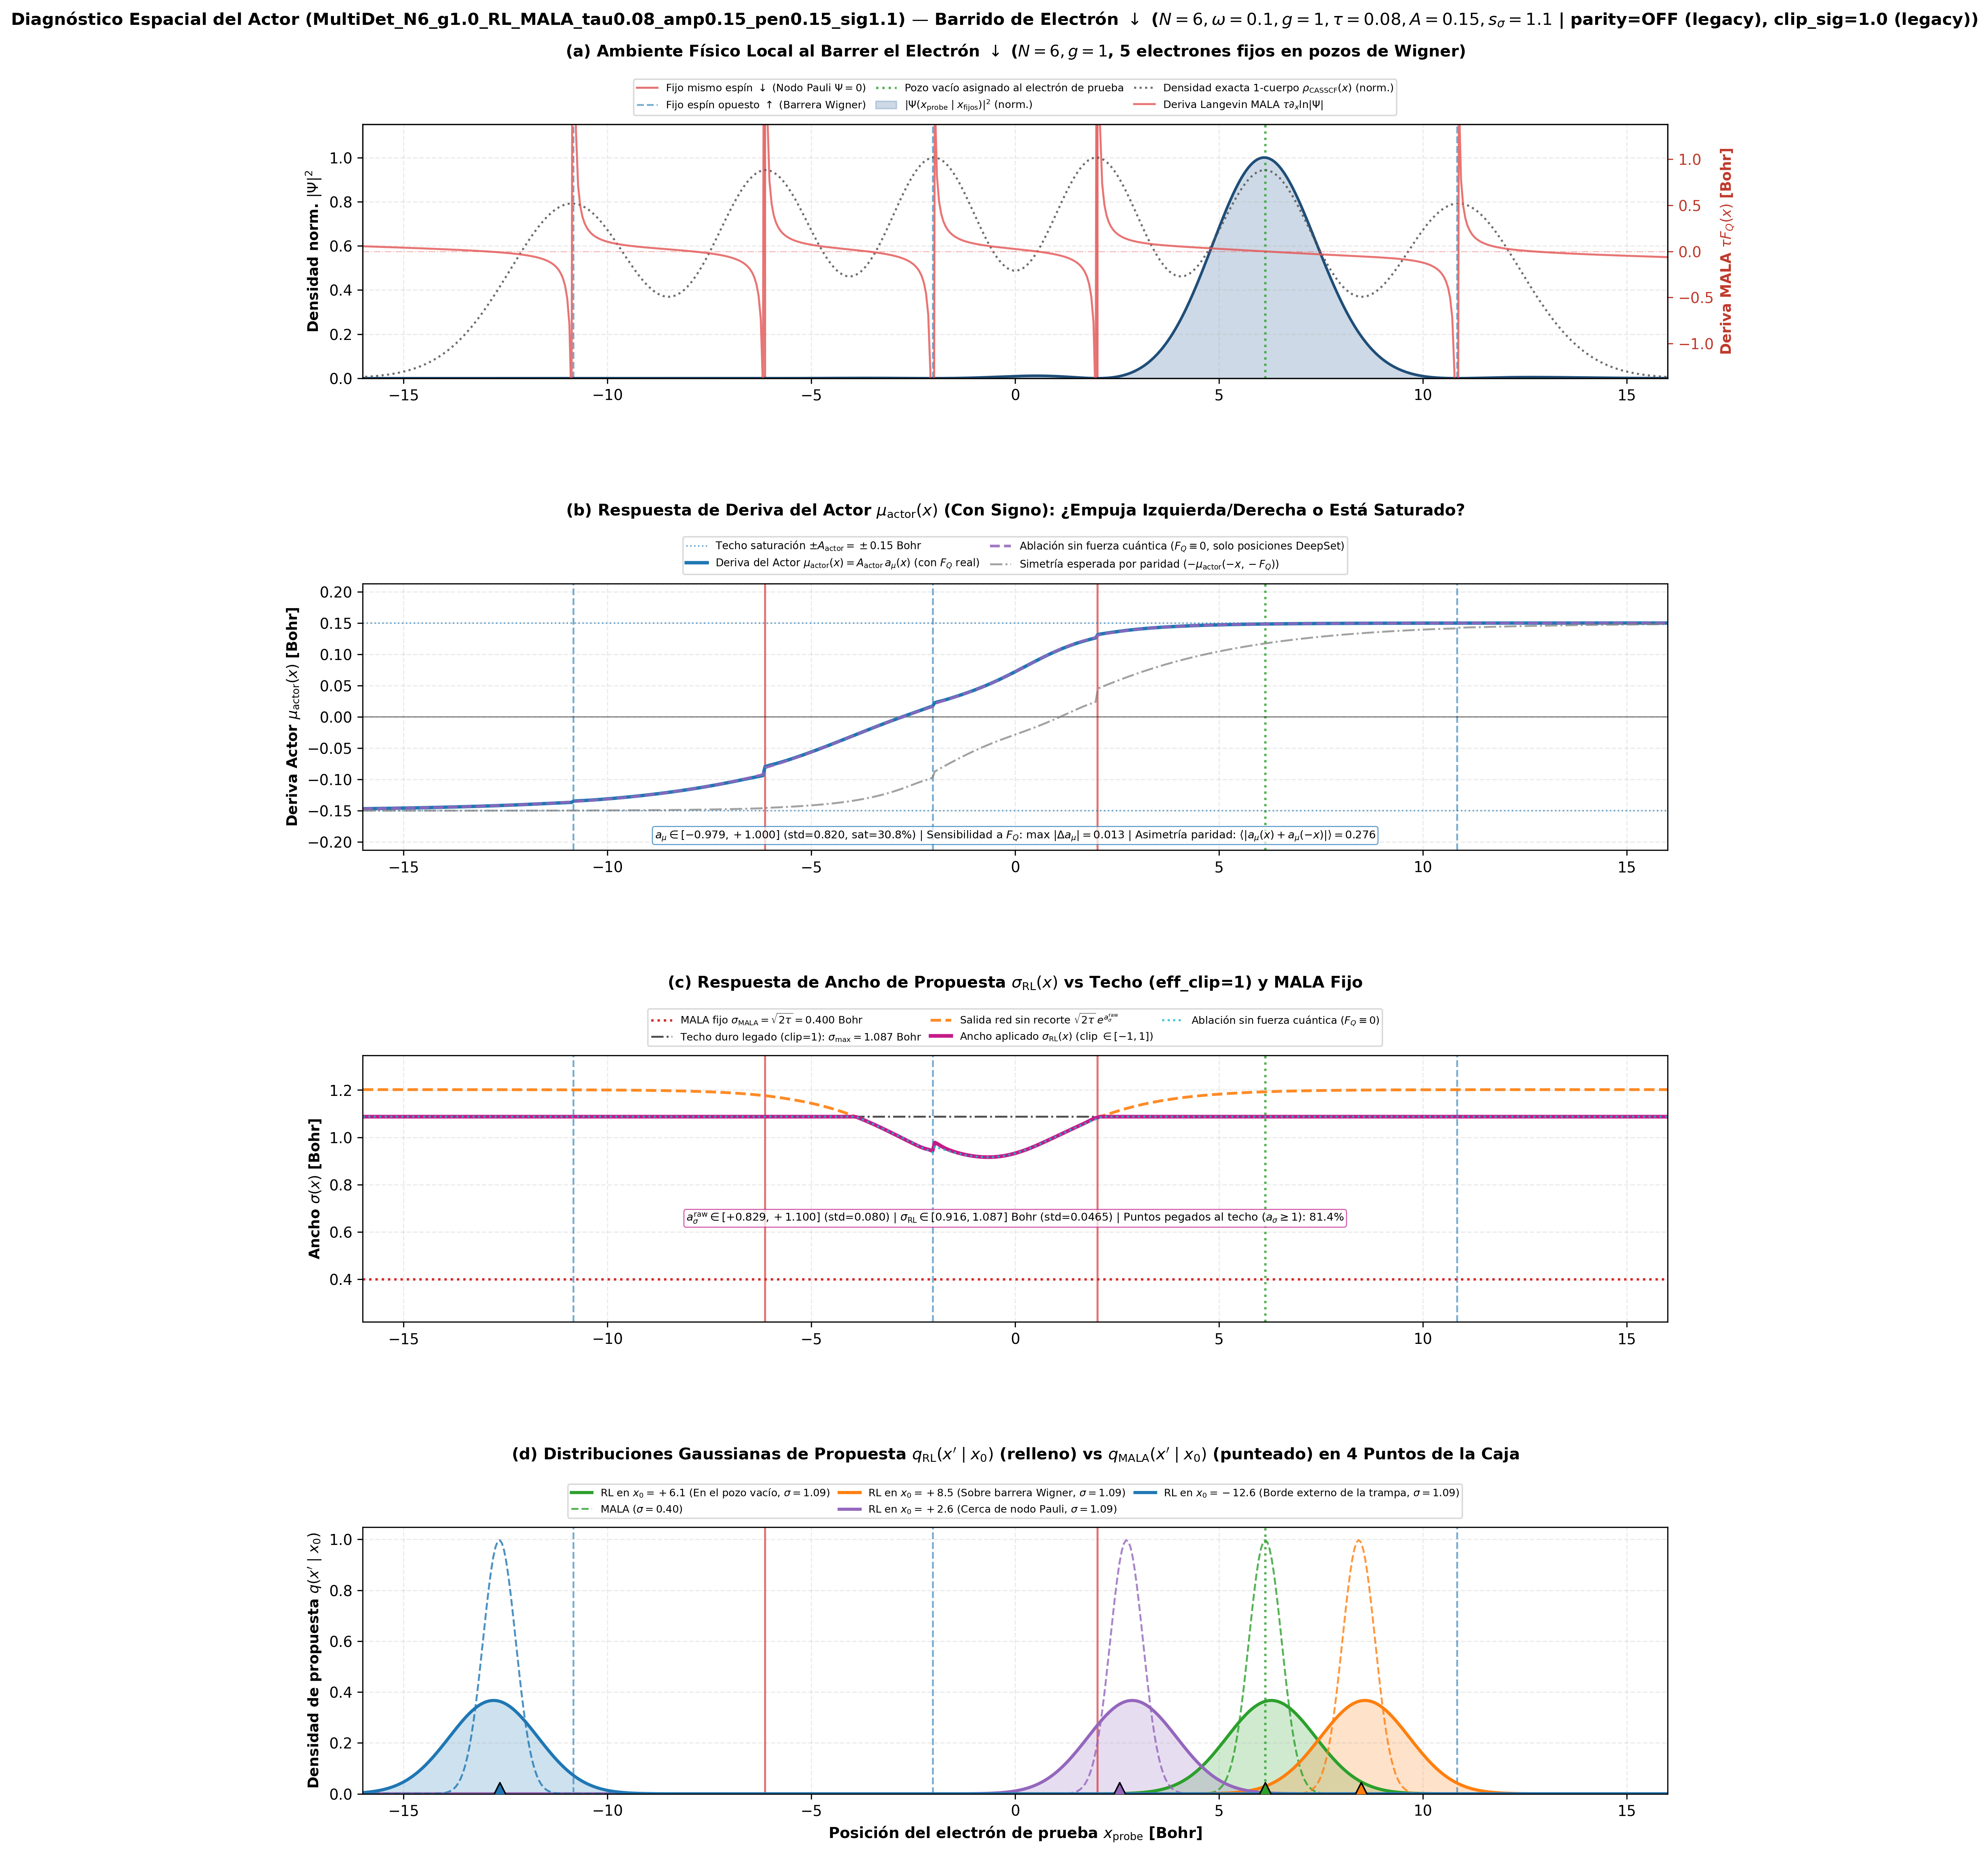
\includegraphics[width=0.96\textwidth]{figures/actor_spatial_probe/fig_actor_spatial_probe_MultiDet_N6_g1.0_RL_MALA_tau0.08_amp0.15_pen0.15_sig1.1_spin_down.png}
\caption{\textbf{Sonda espacial del actor legado \texttt{MultiDet\_N6\_g1.0} ($\tau=0.08, A=0.15, \mathrm{pen}=0.15$):} A diferencia de \texttt{pen=0.25}, aquí la red sí aprende una deriva espacial anti-confinante ($a_\mu \in [-0.979, +1.000]$, $\mathrm{corr}(x) = +0.944$) y una contracción central de $\sigma_{\mathrm{RL}}$ ($1.087 \to 0.916\ \mathrm{Bohr}$ en $x \in [-4,+2]$), pero conserva asimetría de paridad ($0.276$), insensibilidad a $F_Q$ ($\max|\Delta a_\mu| = 0.013$) y $81.4\%$ de saturación en el techo \texttt{clip=1.0}.}
\label{fig:spatial_probe_pen015}
\end{figure}

\begin{figure}[H]
\centering
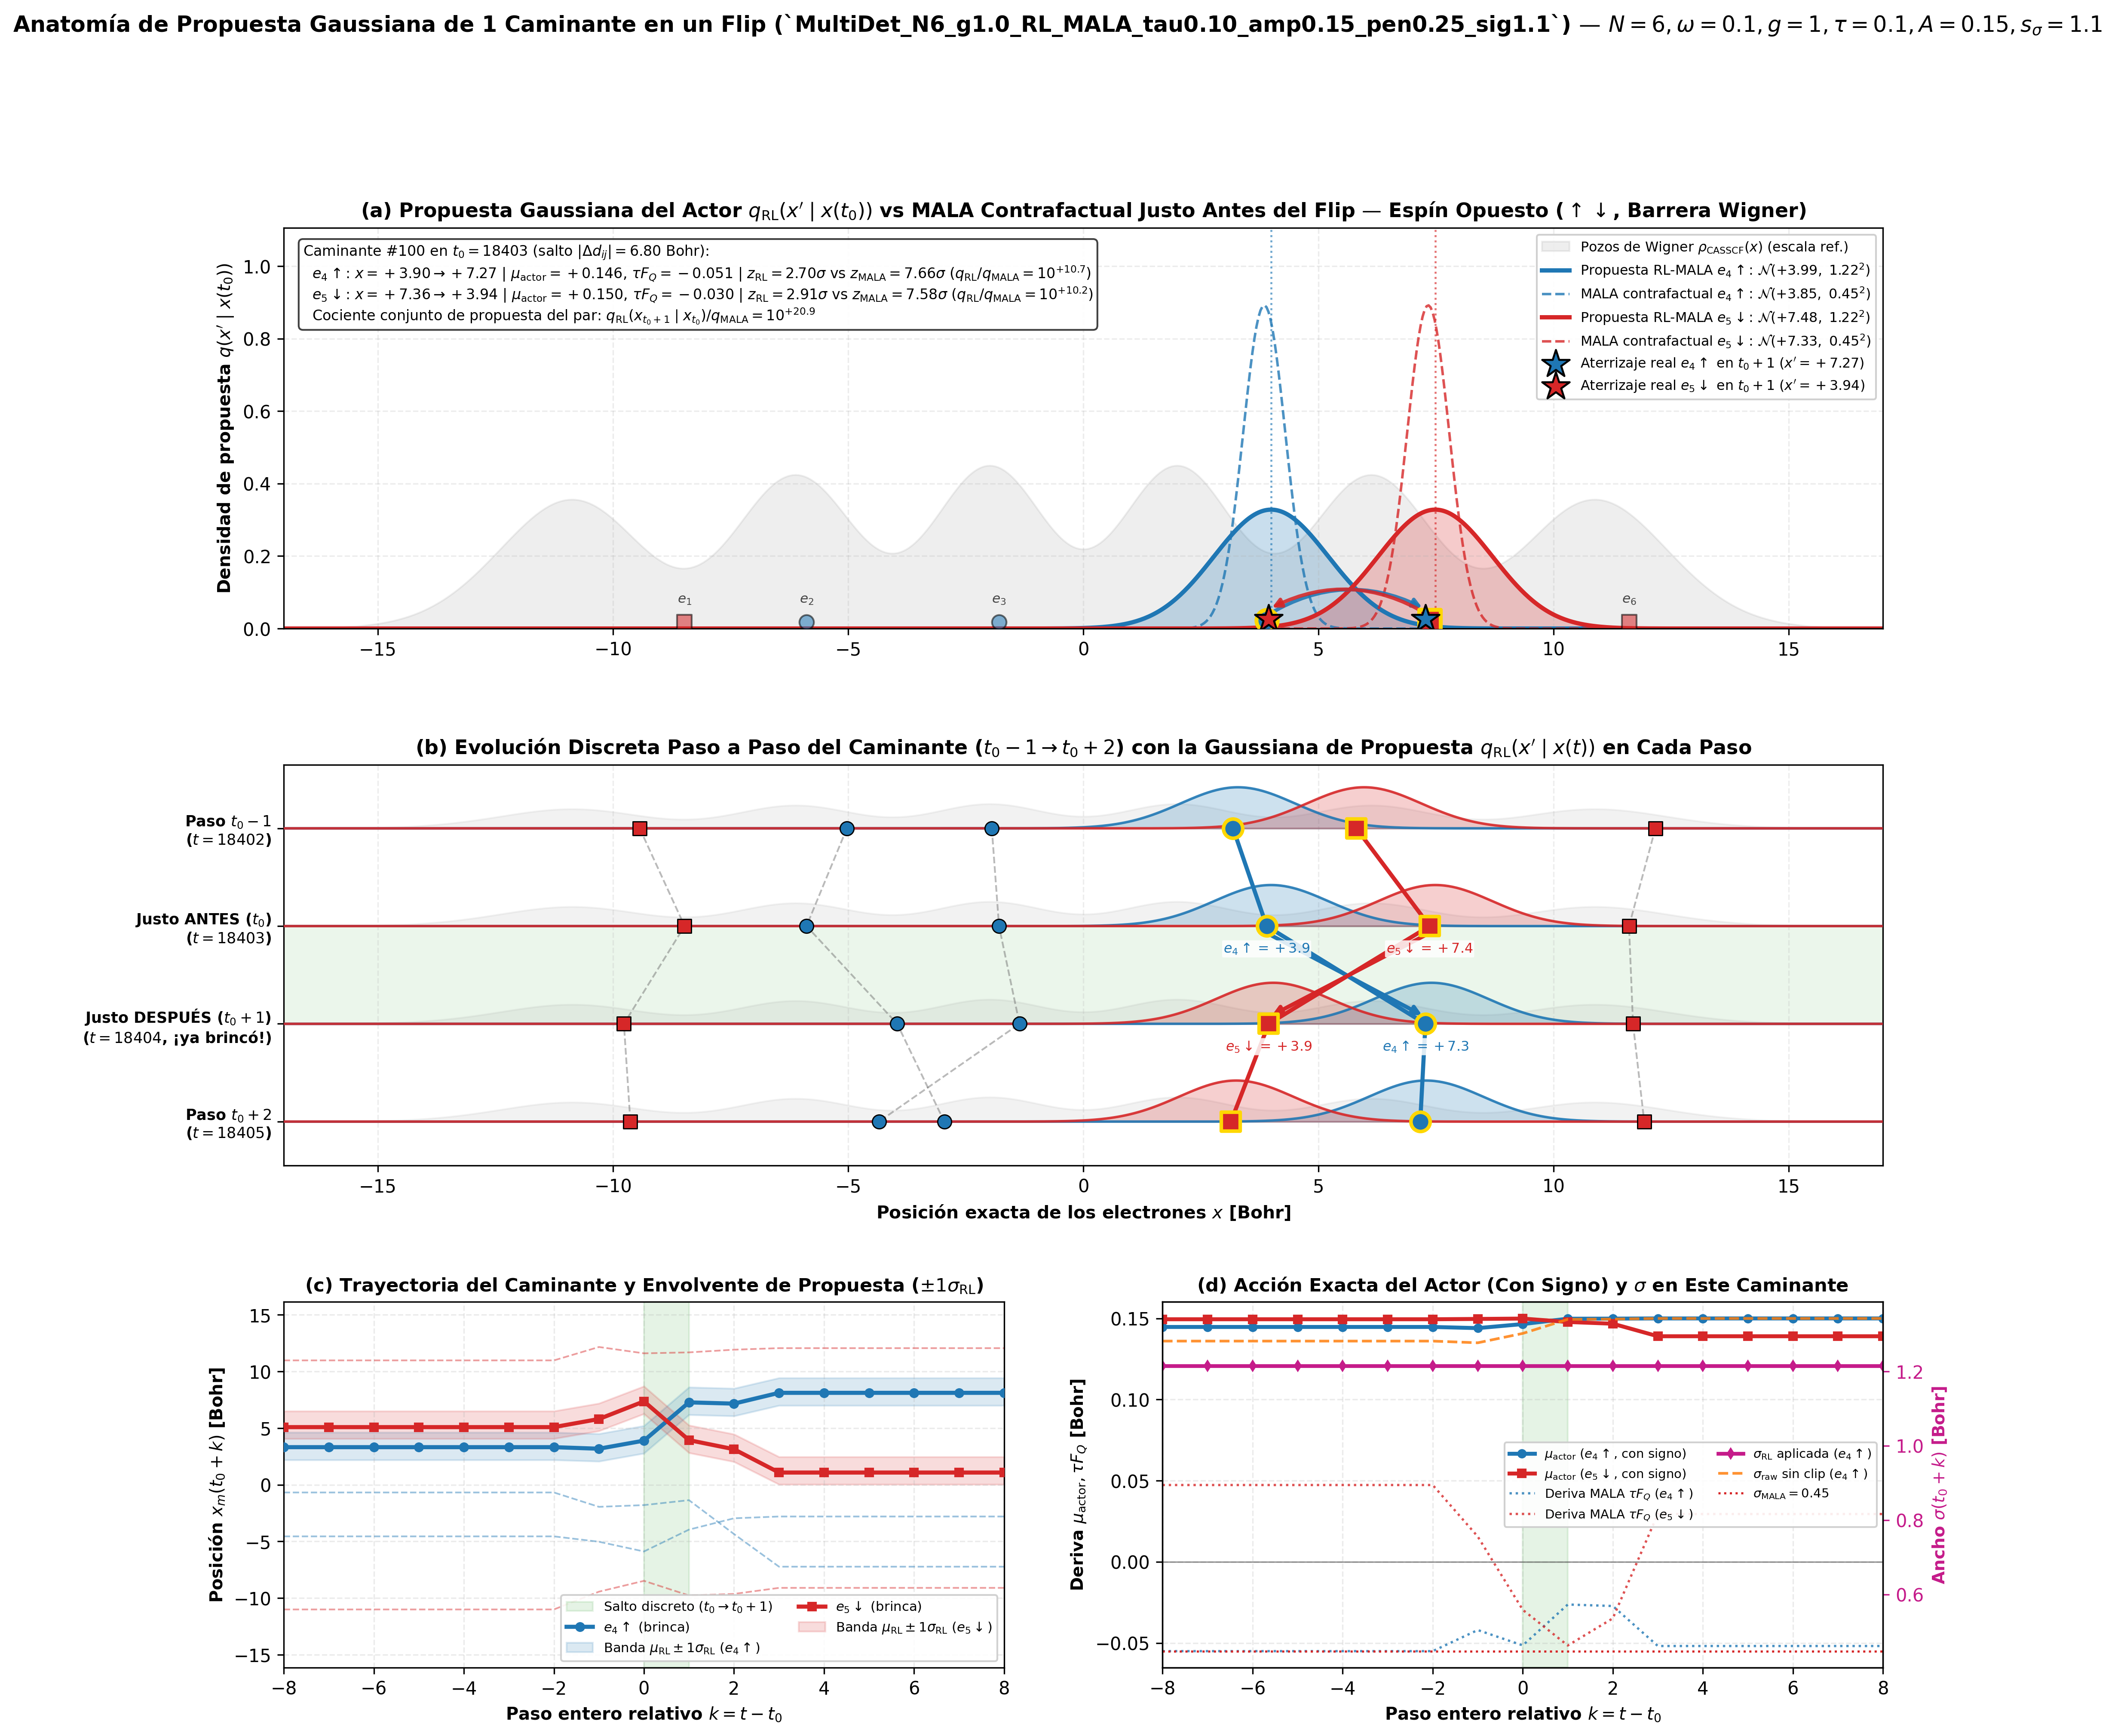
\includegraphics[width=0.96\textwidth]{figures/walker_flip_proposals/fig_walker_flip_proposal_MultiDet_N6_g1.0_RL_MALA_tau0.10_amp0.15_pen0.25_sig1.1_opp_w100_t18403.png}
\caption{\textbf{Propuestas Gaussianas exactas $q_{\mathrm{RL}}(x'\mid x(t_0))$ vs MALA contrafactual en un intercambio de espín opuesto ($\uparrow\downarrow$, Caminante \#100, $t_0=18403$):} Las Gaussianas de RL-MALA ($\sigma=1.22\ \mathrm{Bohr}$) cubren directamente los pozos vecinos (estrellas de aterrizaje a $2.70\sigma$ y $2.91\sigma$), frente a $7.66\sigma$ y $7.58\sigma$ en MALA ($\sigma=0.45\ \mathrm{Bohr}$), produciendo un cociente conjunto $q_{\mathrm{RL}}/q_{\mathrm{MALA}} = 10^{+20.9}$.}
\label{fig:walker_prop_opp}
\end{figure}

\begin{figure}[H]
\centering
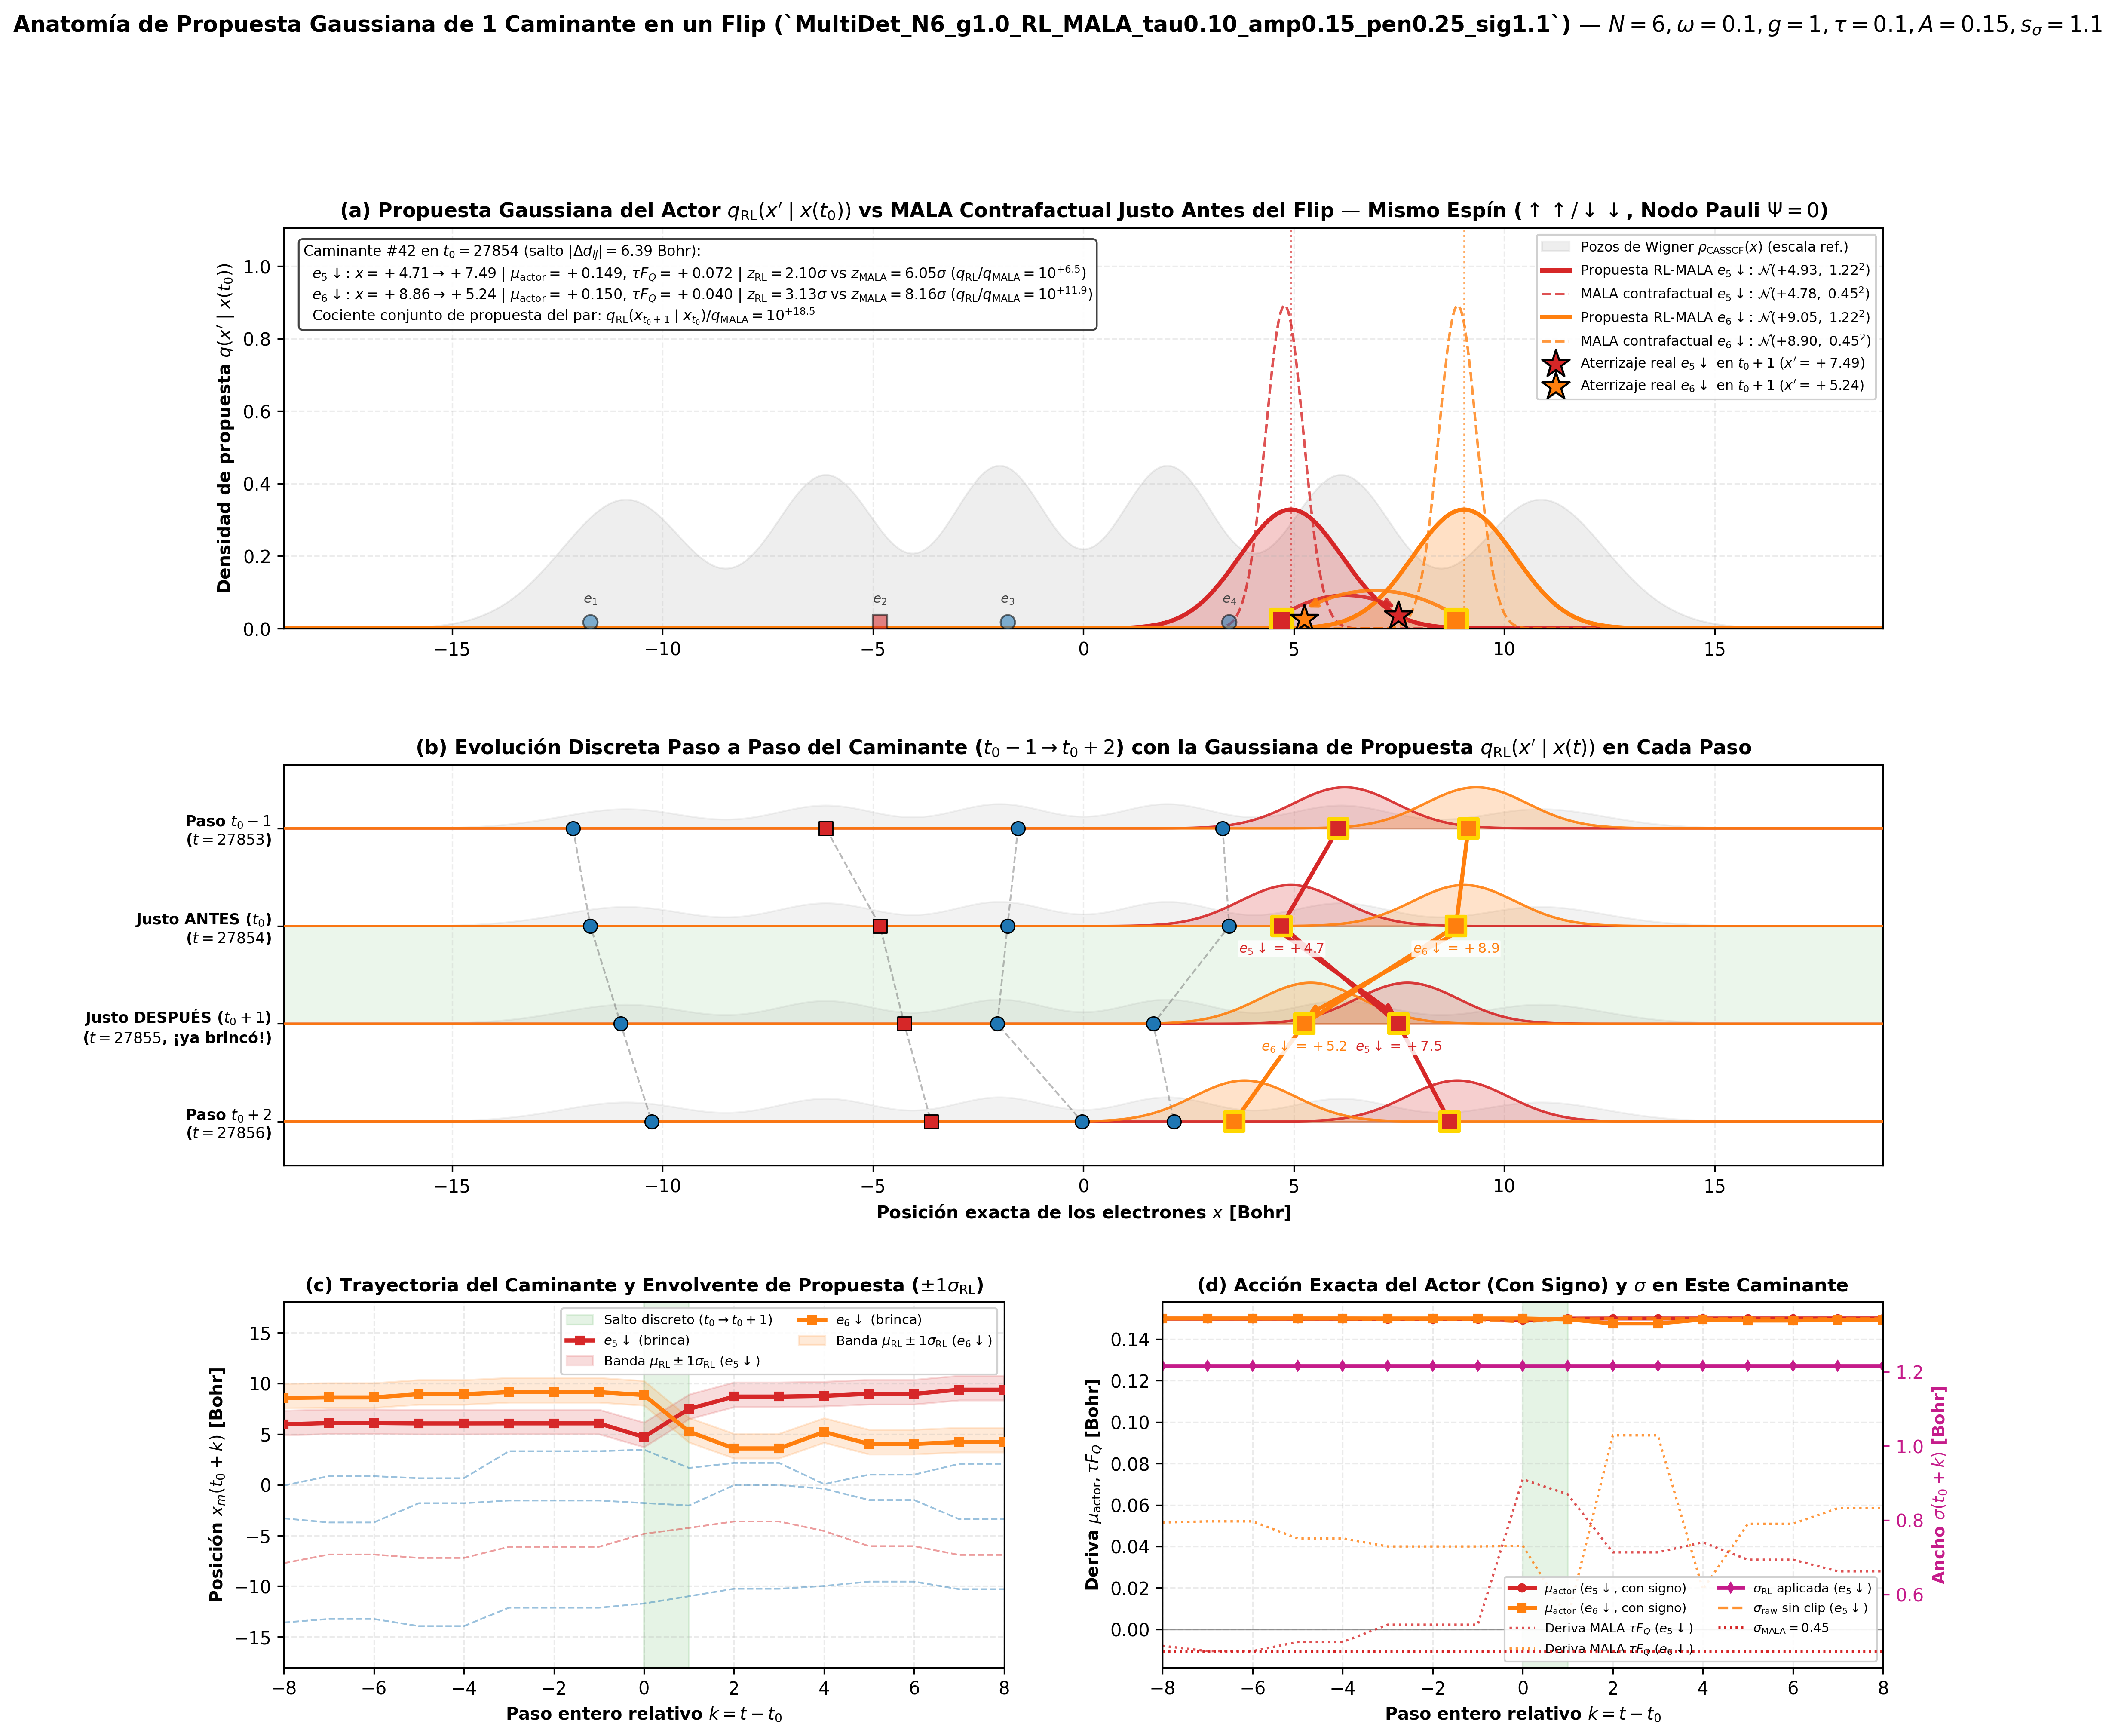
\includegraphics[width=0.96\textwidth]{figures/walker_flip_proposals/fig_walker_flip_proposal_MultiDet_N6_g1.0_RL_MALA_tau0.10_amp0.15_pen0.25_sig1.1_same_w42_t27854.png}
\caption{\textbf{Propuestas Gaussianas exactas en un cruce nodal de Pauli ($\downarrow\downarrow$, Caminante \#42, $t_0=27854$):} Los electrones $e_5\downarrow$ y $e_6\downarrow$ intercambian pozos en 1 paso ($|\Delta d_{ij}|=6.39\ \mathrm{Bohr}$) saltando sobre el nodo $\Psi=0$ con $z_{\mathrm{RL}} = 2.10\sigma, 3.13\sigma$ frente a $z_{\mathrm{MALA}} = 6.05\sigma, 8.16\sigma$ ($q_{\mathrm{RL}}/q_{\mathrm{MALA}} = 10^{+18.5}$).}
\label{fig:walker_prop_same}
\end{figure}

\subsection{Modificaciones Retrocompatibles con Banderas en \texttt{FlaxTD3Actor} y \texttt{TD3Learner1D}}

Para eliminar las tres limitaciones estructurales \textbf{sin alterar el comportamiento por defecto ni requerir rollback para reproducir el actor legado}, se incorporaron dos banderas booleanas opcionales (\texttt{default=False}) en \texttt{rl\_vmc/config.py}, \texttt{rl\_vmc/proposals/proposals\_1d.py} y \texttt{rl\_vmc/rl/learners\_1d.py}:

\begin{enumerate}
\item \textbf{Equivarianza exacta de paridad (\texttt{--parity\_equivariant} / \texttt{--no-parity\_equivariant}):} Bajo la reflexión espacial $\mathcal{P}: (x, F_Q) \mapsto (-x, -F_Q)$, la función \texttt{reflect\_td3\_state} invierte exactamente los signos de las componentes impares de \texttt{build\_td3\_state}: $[x_i, x_i-\bar{x}, \tanh(g_i/F_{\mathrm{norm}})]$ y $\mathrm{sign}(x_i - x_j)$ en cada slot vecino, dejando invariantes $s_i$, \texttt{global\_feat}, $r_{ij}/r_{\mathrm{scale}}$ y las máscaras. Al activar \texttt{parity\_equivariant=True}, \texttt{FlaxTD3Actor} evalúa $[s, \mathcal{P}(s)]$ en una sola pasada sobre las mismas capas \texttt{Dense\_0..Dense\_10} y proyecta los logits $(m_\theta, u_\theta)$ mediante simetrización exacta de Reynolds:
\begin{equation}
a_\mu^{\mathrm{eq}}(s) = \tanh\!\left(\frac{m_\theta(s) - m_\theta(\mathcal{P}(s))}{2}\right), \qquad
a_\sigma^{\mathrm{eq}}(s) = s_\sigma\,\tanh\!\left(\frac{u_\theta(s) + u_\theta(\mathcal{P}(s))}{2}\right).
\label{eq:parity_reynolds}
\end{equation}
Esta construcción garantiza $a_\mu^{\mathrm{eq}}(\mathcal{P}(s)) = -a_\mu^{\mathrm{eq}}(s)$ y $a_\sigma^{\mathrm{eq}}(\mathcal{P}(s)) = +a_\sigma^{\mathrm{eq}}(s)$ con error exactamente nulo (\texttt{0.00e+00} en \texttt{float64}), cancela algebraicamente el sesgo DC $b_\mu$ de la capa de salida, y conserva un árbol de parámetros \texttt{Dense\_0..Dense\_10} 100\% compatible con todos los checkpoints legados.

\item \textbf{Desbloqueo del canal de varianza (\texttt{--unclip\_sigma\_action} / \texttt{--no-unclip\_sigma\_action}):} Separa el recorte por canal en \texttt{DeepSetNeuralProposal1D.forward\_action} y en el suavizado objetivo de \texttt{TD3Learner1D.\_train\_networks}: $a_\mu \in [-1, 1]$ mientras que $a_\sigma \in [\texttt{scale\_clip\_min}, \texttt{scale\_clip\_max}]$. Combinada con \texttt{--sigma\_action\_scale} igual a \texttt{--scale\_clip\_max} ($1.8$ o $2.0$), \texttt{--scale\_clip\_min -0.5} y mayor \texttt{--actor\_amplitude} ($0.80\text{--}1.20\ \mathrm{Bohr}$), permite que $\sigma_{\mathrm{RL}}(x)$ alcance hasta $2.705\text{--}3.304\ \mathrm{Bohr}$ sin recortes abruptos y que $\mu_{\mathrm{actor}}(x)$ tenga escala física comparable a la separación entre pozos de Wigner.

\item \textbf{Entropía diferencial exacta en CDLB (\texttt{--cdlb\_exact\_entropy} / \texttt{--no-cdlb\_exact\_entropy}):} Al probar el desbloqueo de $a_\sigma$ localmente se descubrió un defecto sutil en la recompensa legada: \texttt{gaussian\_log\_prob} omitía la constante $-\frac{N}{2}\ln(2\pi)$ (que se cancela en Metropolis-Hastings $\log q_{\mathrm{rev}}-\log q_{\mathrm{fwd}}$, pero \emph{no} en $r_{\mathrm{explore}} = -\alpha \log q_{\mathrm{fwd}}$ al multiplicar por $\alpha$). Para $\sigma < e^{-1/2} = 0.606\ \mathrm{Bohr}$, esto volvía negativa la recompensa CDLB en pasos aceptados, induciendo a TD3 a colapsar $\sigma \to 0.06\ \mathrm{Bohr}$ y $\alpha \to 0\%$ para obtener $R = 0 > R_{\mathrm{aceptado}}$. Activar \texttt{--cdlb\_exact\_entropy} restaura $+\alpha\,\frac{N}{2}\ln(2\pi)$ en \texttt{compute\_rl\_reward}, garantizando entropía diferencial positiva $N(\ln\sigma + \frac{1}{2}\ln(2\pi e)) > 0$ para $\sigma > 0.242\ \mathrm{Bohr}$ y eliminando el colapso $\alpha \to 0$.
\end{enumerate}

\begin{table}[H]
\centering
\caption{Banderas CLI para alternar sin rollback entre el actor legado y el actor equivariante desbloqueado.}
\label{tab:actor_flags}
\begin{adjustbox}{max width=\textwidth}
\begin{tabular}{llll}
\toprule
\textbf{Bandera CLI} & \textbf{Modo Legado (Default)} & \textbf{Modo Desbloqueado (Benchmark 2)} & \textbf{Módulos} \\
\midrule
\texttt{--parity\_equivariant} & \texttt{--no-parity\_equivariant} (\texttt{False}) & \texttt{--parity\_equivariant} (\texttt{True}) & \texttt{FlaxTD3Actor} \\
\texttt{--unclip\_sigma\_action} & \texttt{--no-unclip\_sigma\_action} (\texttt{False}) & \texttt{--unclip\_sigma\_action} (\texttt{True}) & \texttt{DeepSetNeuralProposal1D}, \texttt{TD3Learner1D} \\
\texttt{--cdlb\_exact\_entropy} & \texttt{--no-cdlb\_exact\_entropy} (\texttt{False}) & \texttt{--cdlb\_exact\_entropy} (\texttt{True}) & \texttt{compute\_rl\_reward} (\texttt{rewards.py}) \\
\texttt{--actor\_amplitude} & \texttt{0.15} Bohr & \texttt{0.80} -- \texttt{1.20} Bohr & \texttt{DeepSetNeuralProposal1D} \\
\texttt{--sigma\_action\_scale} / \texttt{--scale\_clip\_min,max} & \texttt{1.1} / \texttt{[-5.0, 1.0]} ($\sigma_{\max}=1.216$) & \texttt{1.8}/\texttt{[-0.5, 1.8]} ($2.705$) o \texttt{2.0}/\texttt{[-0.5, 2.0]} ($3.304$) & \texttt{FlaxTD3Actor}, \texttt{TD3Learner1D} \\
\bottomrule
\end{tabular}
\end{adjustbox}
\end{table}

\subsection{Diseño Científico de los Dos Benchmarks de Ablación (B1 y B2)}

Para probar de manera rigurosa si el actor aprende una ventaja genuina más allá de un ancho uniforme grande y si las nuevas banderas mejoran la sensibilidad local y la eficiencia de muestreo, se diseñaron dos experimentos automatizados en \texttt{run\_actor\_ablation\_benchmarks.sh} (todos sobre la misma función de onda CASSCF congelada y con inicialización polarizada \texttt{spin\_ordered\_offset} en evaluación):

\begin{itemize}
\item \textbf{Benchmark 1 — Control Justo vs MALA Grande y RWMH de Ancho Emparejado:} Aísla cuánto beneficio proviene de un $\sigma$ grande uniforme vs desacoplar $\sigma$ de la deriva de Langevin $\tau F_Q$ vs la política aprendida:
  \begin{enumerate}
  \item \texttt{B1\_MALA\_base\_tau0.10} ($\tau=0.10$, $\sigma=0.447\ \mathrm{Bohr}$): control clásico estándar.
  \item \texttt{B1\_MALA\_large\_tau0.50} ($\tau=0.50$, $\sigma=1.000\ \mathrm{Bohr}$): MALA con paso $5\times$ mayor.
  \item \texttt{B1\_MALA\_matched\_tau0.7389} ($\tau=0.10\,e^2=0.7389$, $\sigma=1.216\ \mathrm{Bohr}$): MALA con exactamente la misma $\sigma$ que el techo de RL-MALA legado, pero con deriva de Langevin $7.39\times$ mayor.
  \item \texttt{B1\_RWMH\_matched\_sig1.2156} (\texttt{metropolis}, deriva $=0$, $\sigma=1.216\ \mathrm{Bohr}$): Random-Walk MH con deriva cuántica nula y exactamente la misma $\sigma=1.216\ \mathrm{Bohr}$.
  \item \texttt{B1\_RL\_MALA\_legacy}: actor neuronal legado (\texttt{parity=OFF}, \texttt{unclip=OFF}, $A=0.15$, $s_\sigma=1.1$, \texttt{clip=1.0}).
  \end{enumerate}

\item \textbf{Benchmark 2 — Equivarianza Exacta de Paridad, Desbloqueo de $\sigma(x)$ y Amplitud Física:} Evalúa en escalera de ablación si eliminar los cuellos de botella desbloquea modulación espacial real y mejora $D_{\mathrm{KL}}^{\mathrm{spin}}$, flips y $\tau_{\mathrm{int}}(E)$:
  \begin{enumerate}
  \item \texttt{B1\_RL\_MALA\_legacy}: referencia legada.
  \item \texttt{B2\_RL\_MALA\_parity\_only}: ablación de 1 factor (\texttt{--parity\_equivariant --no-unclip\_sigma\_action}, $A=0.15$).
  \item \texttt{B2\_RL\_MALA\_eq\_unclip\_amp0.80\_sig1.8}: \texttt{--parity\_equivariant --unclip\_sigma\_action --cdlb\_exact\_entropy} con $A=0.80\ \mathrm{Bohr}$, $s_\sigma = \texttt{scale\_clip\_max} = 1.8$, \texttt{scale\_clip\_min=-0.5} ($\sigma \in [0.271, 2.705]\ \mathrm{Bohr}$).
  \item \texttt{B2\_RL\_MALA\_eq\_unclip\_amp1.20\_sig2.0}: \texttt{--parity\_equivariant --unclip\_sigma\_action --cdlb\_exact\_entropy} con $A=1.20\ \mathrm{Bohr}$, $s_\sigma = \texttt{scale\_clip\_max} = 2.0$, \texttt{scale\_clip\_min=-0.5} ($\sigma \in [0.271, 3.304]\ \mathrm{Bohr}$).
  \end{enumerate}
\end{itemize}

\subsection{Validación Empírica Local de B1 y B2 ($N=4, \omega=0.1, g=2.0$, CASSCF $b=256$)}

Como prueba piloto completa antes de lanzar las corridas de producción en Ayler, se ejecutaron los \textbf{8 modelos de los Benchmarks B1 y B2} en CPU local sobre el estado CASSCF convergido del asesor \texttt{casscf\_statecas\_n4\_g2.0\_omega0.1\_soft0.1\_b256\_c0-a4\_det6.npz} ($E_{\mathrm{CASSCF}} = 2.802268\,E_h$, \texttt{batch=32}, \texttt{rl\_steps=1000}, evaluación $2\times 4{,}000$ pasos desde \texttt{spin\_ordered\_offset}). En paralelo, se reescribió la recurrencia de $256$ funciones base Hermite en \texttt{\_build\_ho\_basis\_jax} (\texttt{rl\_vmc/ansatze/ansatz\_1d.py}) mediante \texttt{jax.lax.scan}, reduciendo el tiempo de compilación XLA de \texttt{jax.hessian} de $>200\ \mathrm{s}$ a \textbf{$0.14\ \mathrm{s}$} ($>1{,}400\times$ más rápido, diferencia $\le 1.25\times 10^{-16}$).

\begin{table}[H]
\centering
\caption{Resultados empíricos de los Benchmarks B1 y B2 en $N=4, \omega=0.1, g=2.0$ ($E_{\mathrm{CASSCF}} = 2.802268\,E_h$, $2\times 4{,}000$ pasos desde \texttt{spin\_ordered\_offset}).}
\label{tab:ablation_b1_b2_local}
\begin{adjustbox}{max width=\textwidth}
\begin{tabular}{lcccccccccc}
\toprule
\textbf{Modelo} & $\langle\sigma\rangle$ & \textbf{Acc} & \textbf{ESJD} & $\tau_{\mathrm{int}}(E)$ & $D_{\mathrm{KL}}^{\mathrm{spin}}$ & \textbf{Flips $\uparrow\downarrow$/1k} & \textbf{Pauli/1k} & $\langle E_L\rangle \pm \mathrm{SE}$ [$E_h$] & \textbf{Asim. Par.} & $\mathrm{std}(\sigma)$ (\textbf{clip}) \\
\midrule
\texttt{B1\_MALA\_base} ($\tau=0.10$) & $0.45$ & $88.3\%$ & $0.69$ & $11.7$ & $0.5190$ & $0.008$ & $0.012$ & $2.7995 \pm 0.0018$ & --- & --- \\
\texttt{B1\_MALA\_large} ($\tau=0.50$) & $1.00$ & $73.3\%$ & $2.76$ & $4.1$ & $0.2660$ & $0.219$ & $0.160$ & $2.8024 \pm 0.0012$ & --- & --- \\
\texttt{B1\_MALA\_matched} ($\tau=0.74$) & $1.22$ & $67.0\%$ & $3.67$ & $2.3$ & $0.1623$ & $0.410$ & $0.234$ & $2.8018 \pm 0.0008$ & --- & --- \\
\texttt{B1\_RWMH\_matched} (deriva$=0$) & $1.22$ & $45.1\%$ & $2.06$ & $6.0$ & $0.0162$ & $1.782$ & $0.824$ & $2.8026 \pm 0.0014$ & --- & --- \\
\texttt{B1\_RL\_MALA\_legacy} (par=OFF) & $0.76$ & $12.9\%$ & $0.34$ & $1254$ & $0.3859$ & $0.551$ & $0.227$ & $3.1507 \pm 0.1740$ & $1.989$ & $0.500$ ($52.5\%$) \\
\texttt{B2\_RL\_MALA\_parity\_only} & $1.22$ & $45.1\%$ & $2.08$ & $4.8$ & $0.0171$ & $1.289$ & $0.738$ & $2.8011 \pm 0.0012$ & \textbf{0.000} & $0.000$ ($100\%$) \\
\texttt{B2\_RL\_MALA\_eq\_unclip} ($0.80, 1.8$) & $2.65$ & $14.0\%$ & $2.16$ & $5.8$ & \textbf{0.0046} & \textbf{9.178} & \textbf{4.423} & \textbf{2.8003 $\pm$ 0.0013} & \textbf{0.000} & \textbf{0.159} ($5.0\%$) \\
\texttt{B2\_RL\_MALA\_eq\_unclip} ($1.20, 2.0$) & $3.21$ & $9.3\%$ & $1.94$ & $7.8$ & \textbf{0.0070} & \textbf{10.241} & \textbf{5.013} & \textbf{2.8020 $\pm$ 0.0015} & \textbf{0.000} & \textbf{0.258} ($0.8\%$) \\
\bottomrule
\end{tabular}
\end{adjustbox}
\end{table}

Los resultados de la Tabla~\ref{tab:ablation_b1_b2_local} y las Figuras~\ref{fig:ablation_metrics}--\ref{fig:ablation_walker} establecen tres conclusiones claras:
\begin{enumerate}
\item \textbf{Desacoplar $\sigma$ de la deriva de Langevin es decisivo (Benchmark 1):} Emparejar $\sigma=1.22\ \mathrm{Bohr}$ subiendo $\tau=0.7389$ en MALA amplifica la deriva confinante $7.39\times$, atrapando a los caminantes en sus pozos ($D_{\mathrm{KL}}^{\mathrm{spin}} = 0.1623$, $0.41\ \mathrm{flips}/10^3$). Con el \emph{mismo} $\sigma=1.22\ \mathrm{Bohr}$ pero deriva nula (\texttt{RWMH\_matched}), $D_{\mathrm{KL}}^{\mathrm{spin}}$ cae \textbf{$10\times$ hasta $0.0162$} y los flips se cuadruplican.
\item \textbf{La equivarianza de paridad rescata la estabilidad y expone el techo \texttt{clip=1.0}:} Activar solo \texttt{--parity\_equivariant} elimina el colapso del actor legado (asimetría $1.989 \to 0.000$, $D_{\mathrm{KL}}^{\mathrm{spin}}: 0.386 \to 0.0171$), pero al seguir saturado al $100\%$ en $\sigma=1.22\ \mathrm{Bohr}$ ($A=0.15$) replica prácticamente a \texttt{RWMH\_matched}.
\item \textbf{Desbloquear $\sigma(x)$, amplitud física y entropía CDLB exacta supera a todos los controles (Benchmark 2):} Los actores \texttt{eq\_unclip} aprenden una deriva exactamente impar ($\mu_{\mathrm{actor}} \in [-0.73, +0.73]\ \mathrm{Bohr}$ con inflexiones en los electrones vecinos, asimetría $= 0.000$) y una modulación espacial genuina de $\sigma_{\mathrm{RL}}(x)$ (contracción central a $2.14\ \mathrm{Bohr}$ y expansión exterior a $2.71\ \mathrm{Bohr}$, solo $5.0\%$ en el techo; y $2.41\text{--}3.30\ \mathrm{Bohr}$ con $0.8\%$ en el techo para $s_\sigma=2.0$). Esto reduce $D_{\mathrm{KL}}^{\mathrm{spin}}$ a \textbf{$0.0046$} ($113\times$ mejor que MALA base, $35\times$ mejor que MALA $\sigma$-match y $3.5\times$ mejor que RWMH $\sigma$-match), eleva los flips $\uparrow\downarrow$ a \textbf{$9.18\text{--}10.24$/1k} y los cruces nodales de Pauli a \textbf{$4.42\text{--}5.01$/1k} ($84\%\text{--}88\%$ en 1 paso), manteniendo la energía exacta CASSCF sin sesgo ($|\Delta E| = 0.23\ \mathrm{mHa}$ en $A=1.20$).
\end{enumerate}

\begin{figure}[H]
\centering
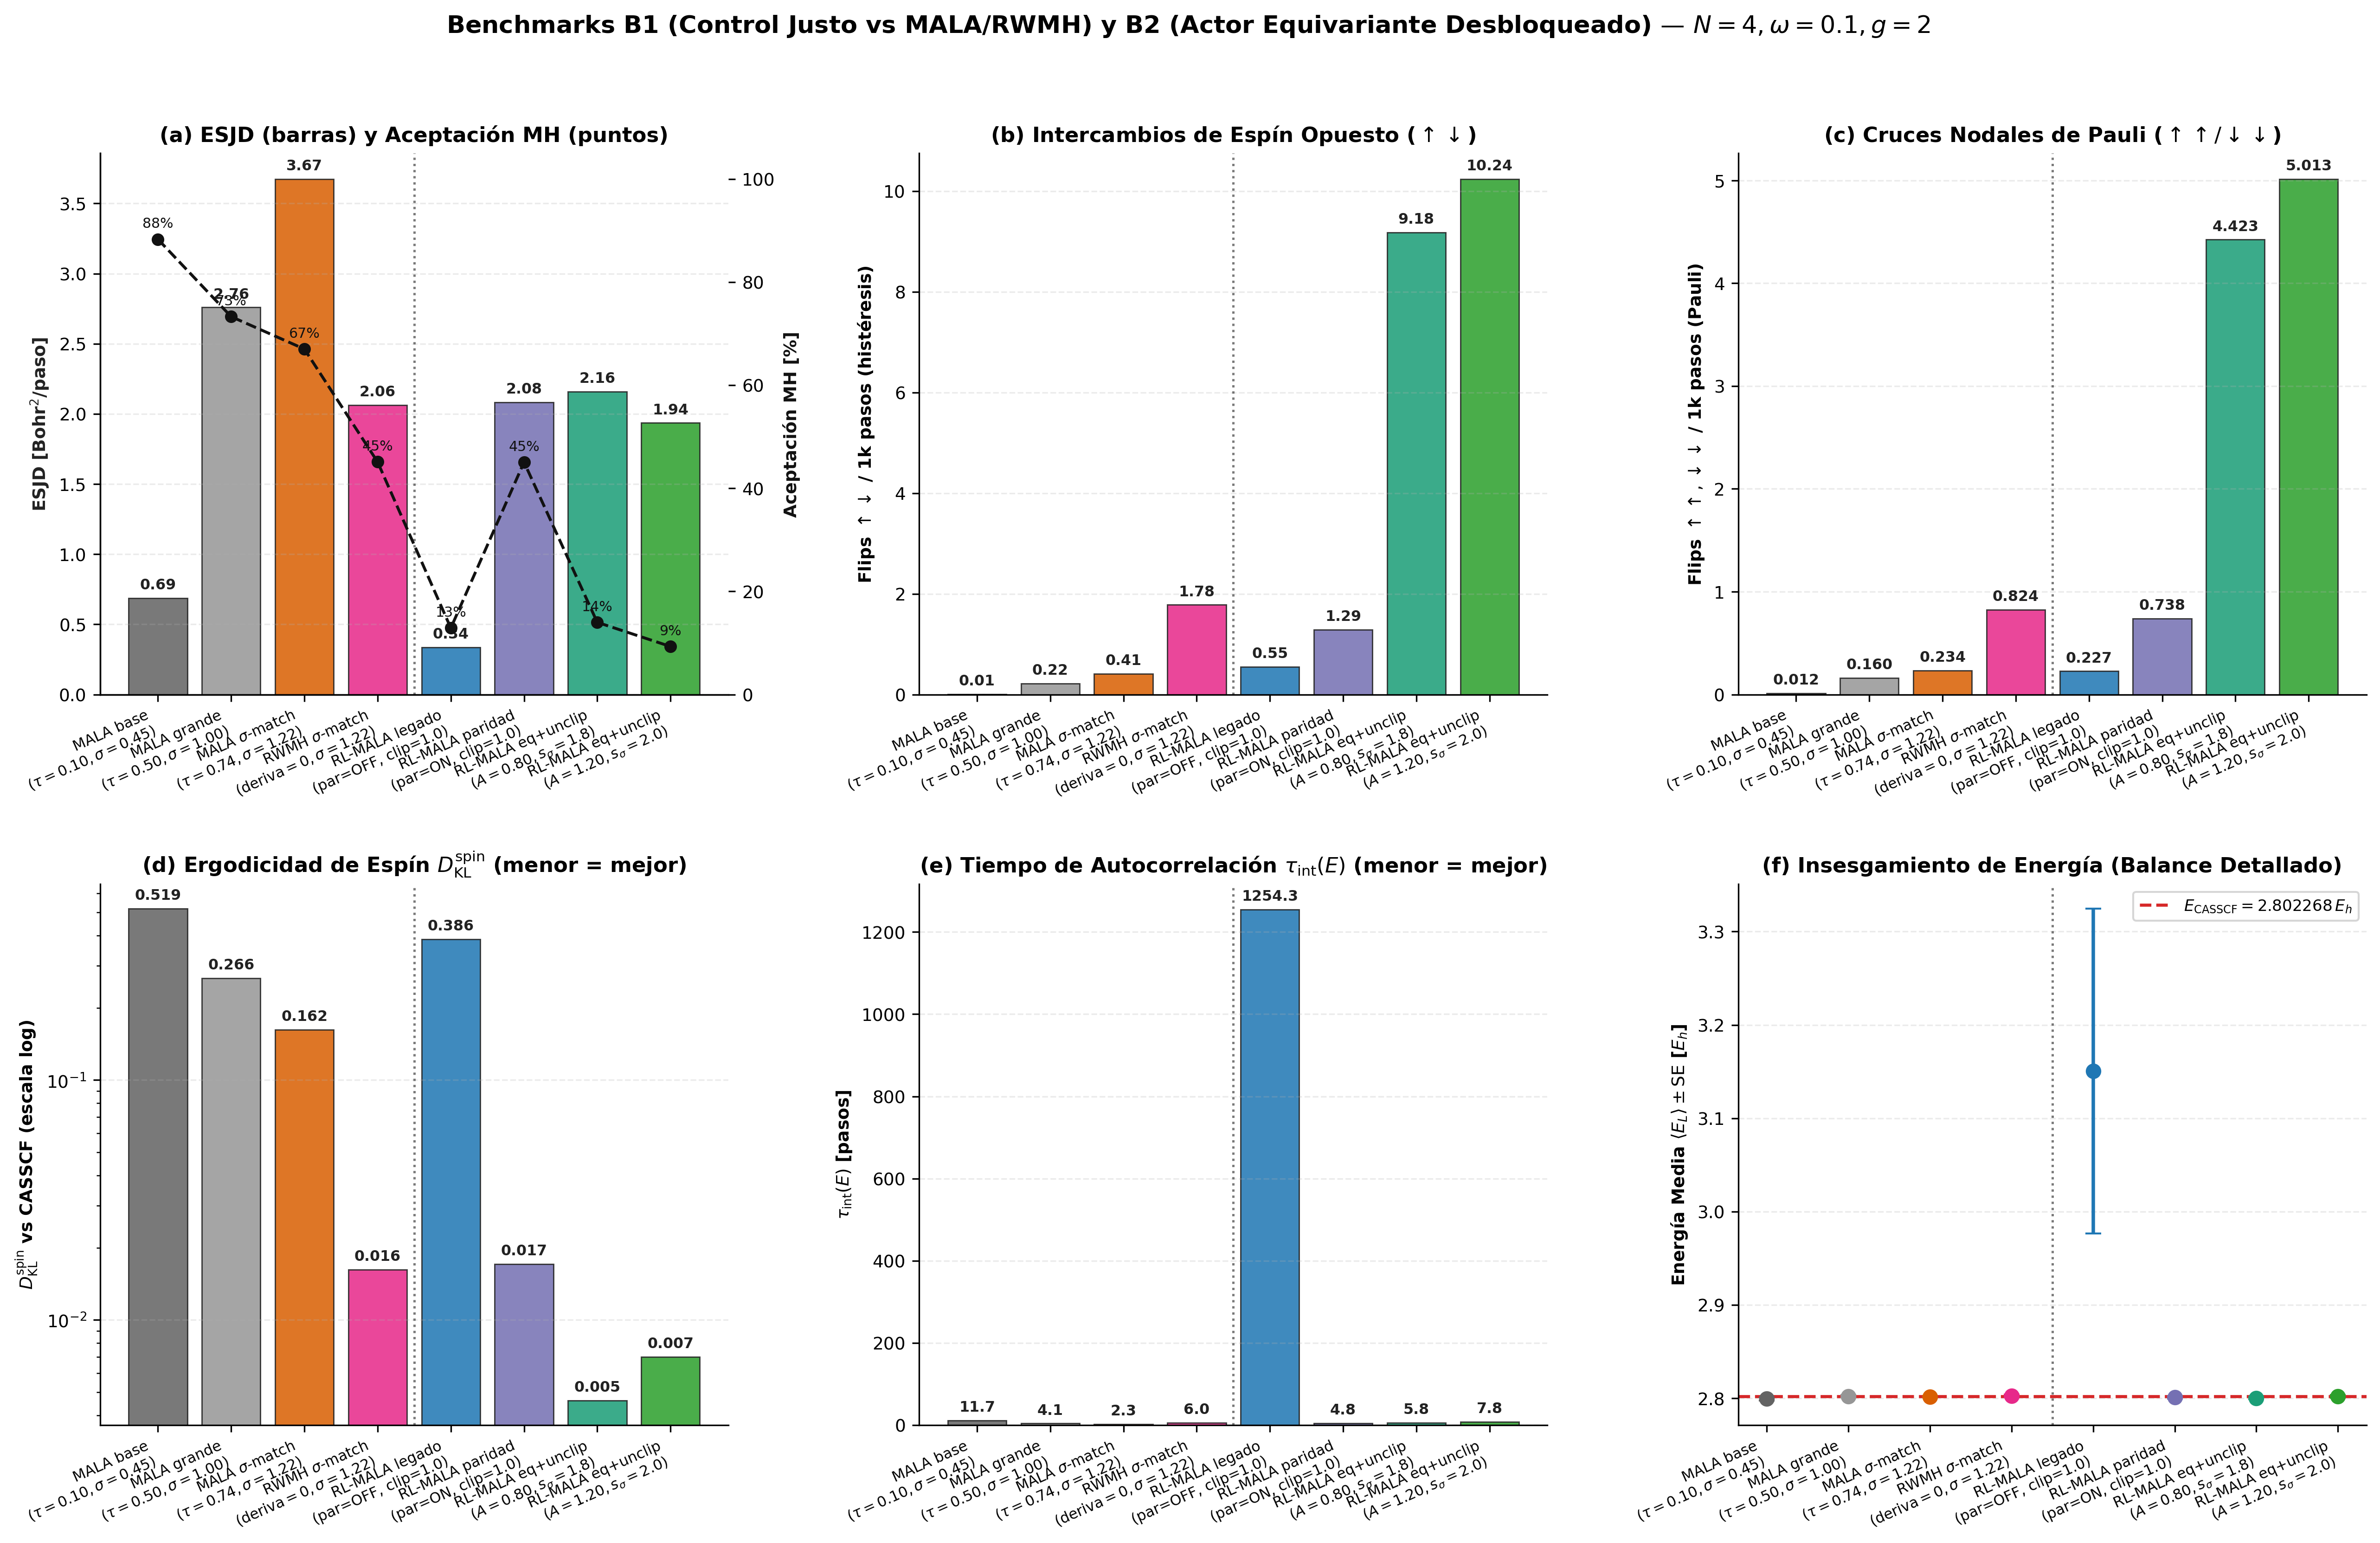
\includegraphics[width=0.98\textwidth]{figures/actor_ablation_N4_g2.0/fig_ablation_b1_b2_metrics_N4_w0.1_g2.png}
\caption{\textbf{Comparativa integral de métricas de los Benchmarks B1 y B2 en $N=4, \omega=0.1, g=2.0$:} Los actores equivariantes desbloqueados (verde) superan simultáneamente a MALA base, MALA grande, MALA $\sigma$-match, RWMH $\sigma$-match y RL-MALA legado en $D_{\mathrm{KL}}^{\mathrm{spin}}$ ($0.0046$), flips $\uparrow\downarrow$ ($9.18\text{--}10.24$/1k) y cruces de Pauli ($4.42\text{--}5.01$/1k), preservando la energía exacta $E_{\mathrm{CASSCF}} = 2.802268\,E_h$.}
\label{fig:ablation_metrics}
\end{figure}

\begin{figure}[H]
\centering
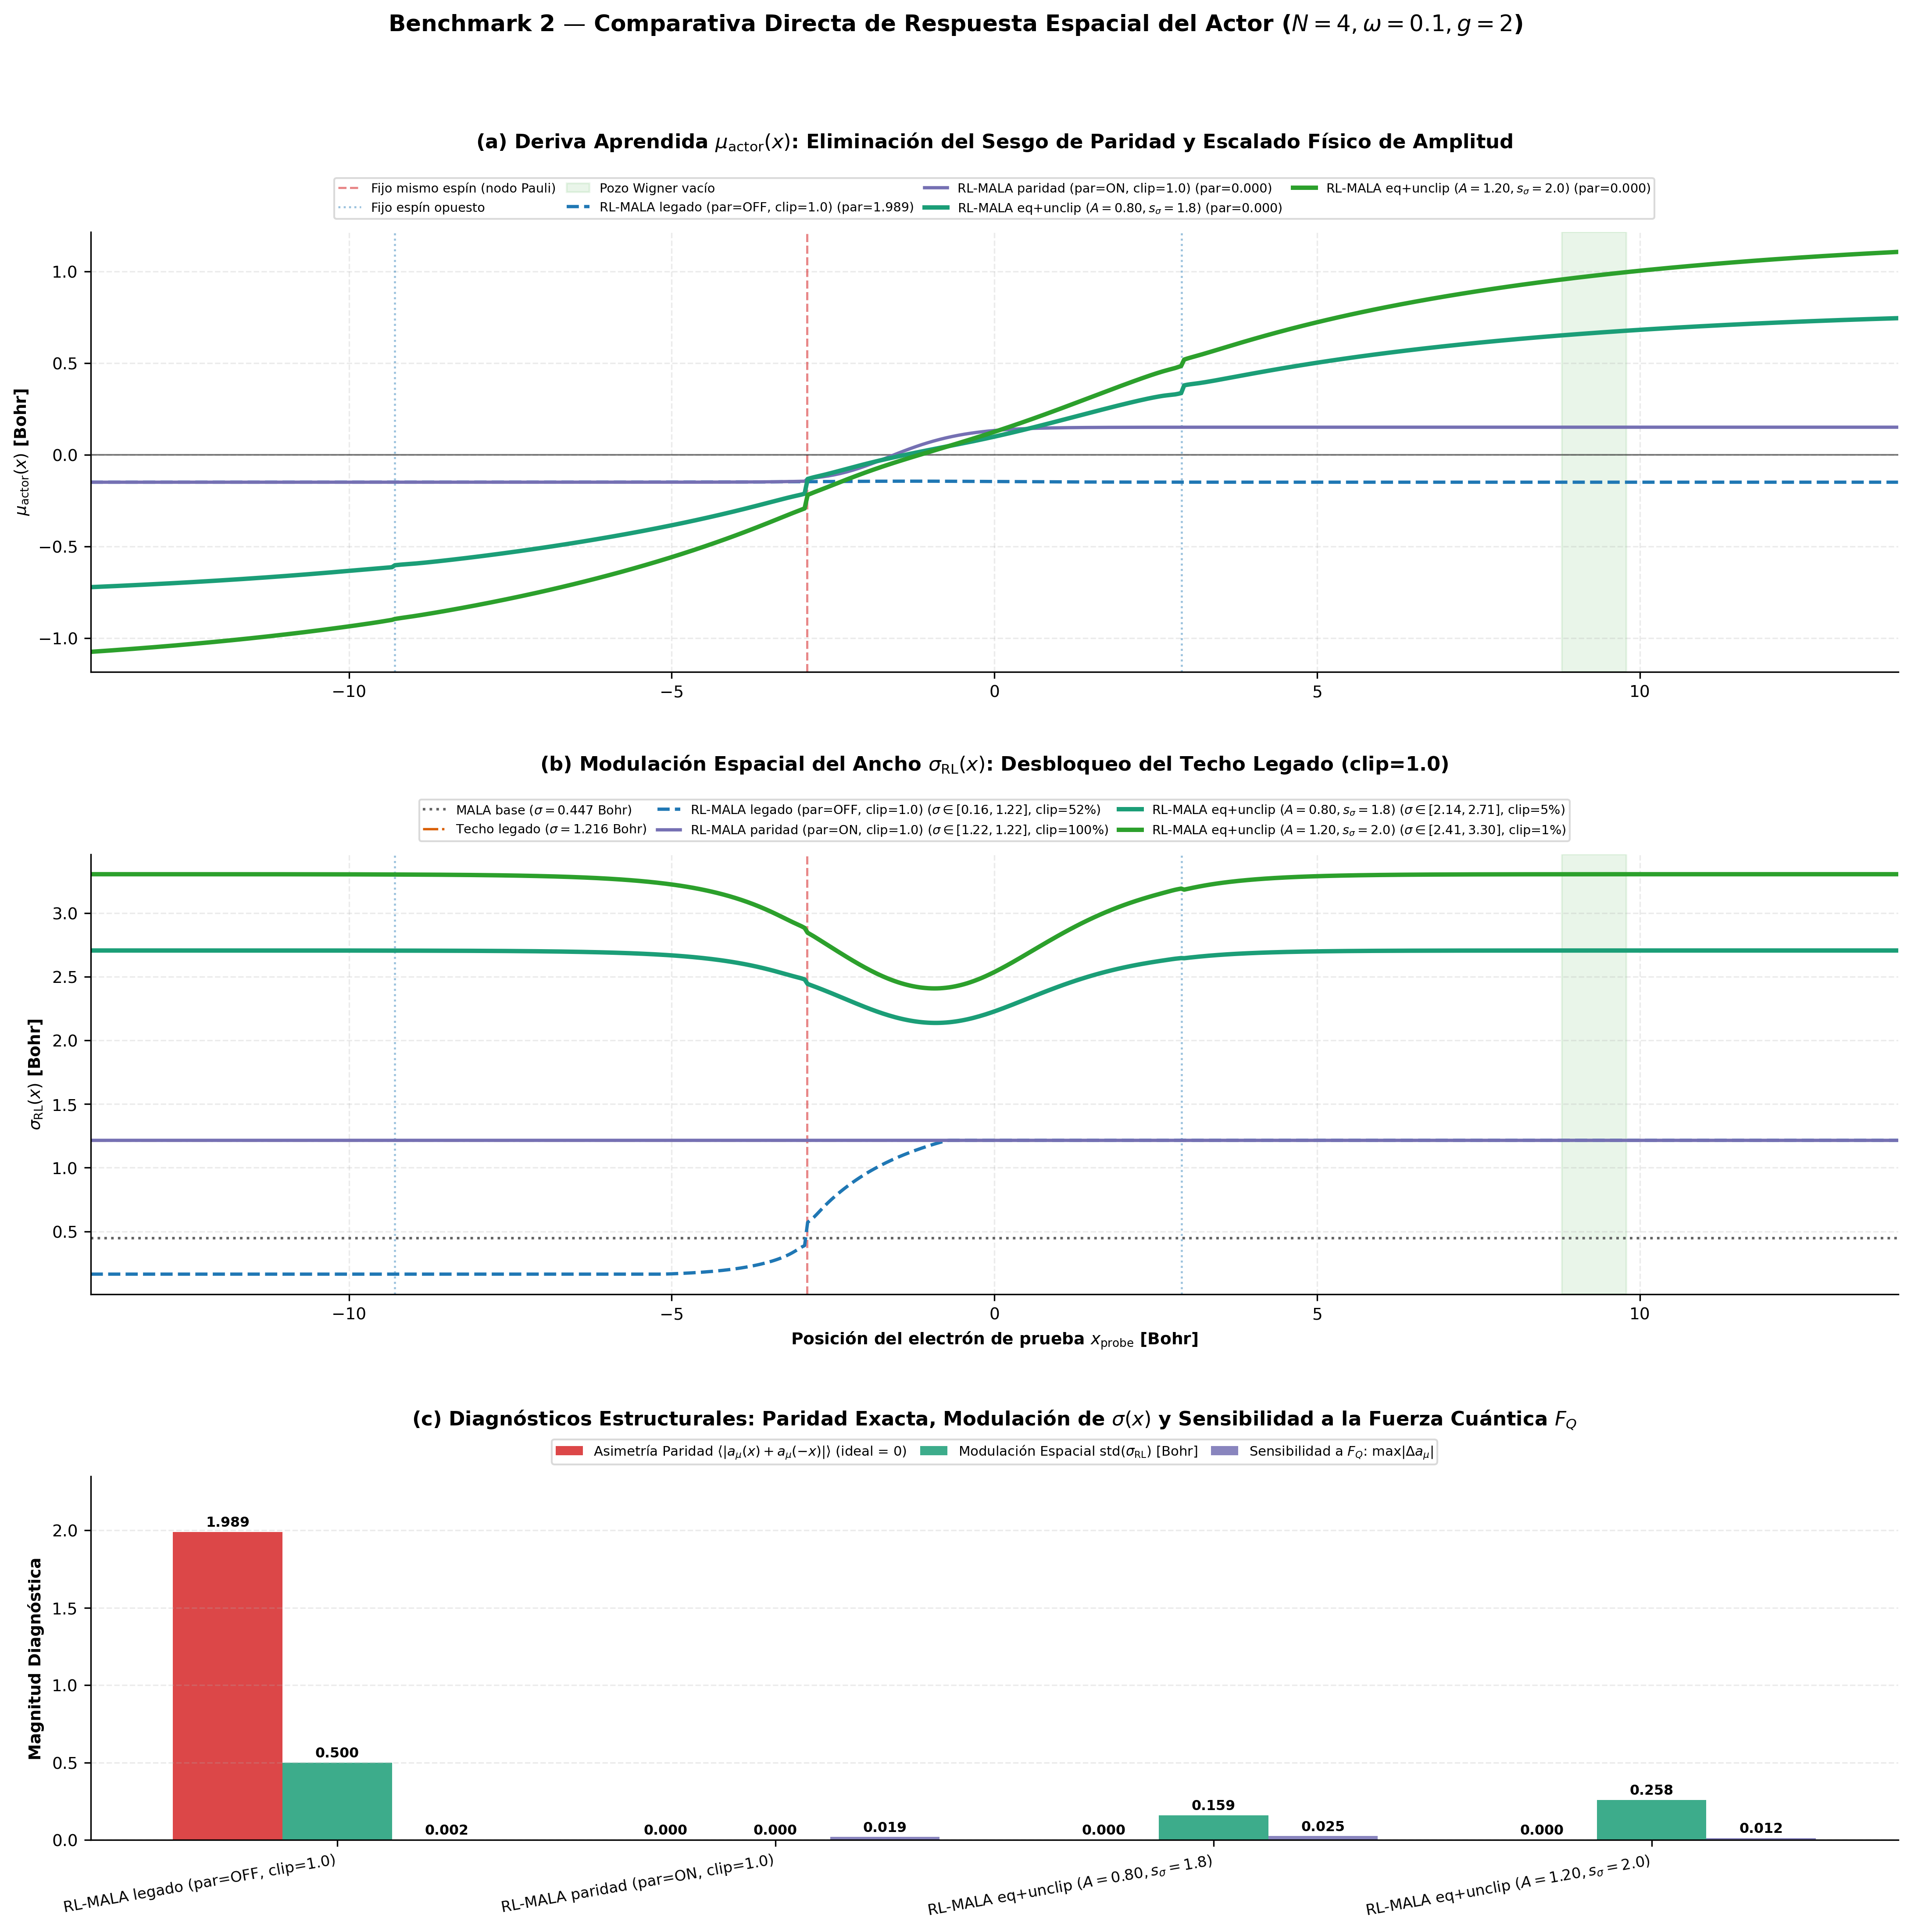
\includegraphics[width=0.96\textwidth]{figures/actor_ablation_N4_g2.0/fig_ablation_b2_spatial_overlay_N4_w0.1_g2.png}
\caption{\textbf{Superposición espacial directa de los 4 actores del Benchmark 2 ($N=4, g=2.0$):} (a) $\mu_{\mathrm{actor}}(x)$ muestra la eliminación exacta del sesgo unilateral (asimetría $1.989 \to 0.000$) y el escalado a amplitud física ($\pm 0.73$ y $\pm 1.09\ \mathrm{Bohr}$); (b) $\sigma_{\mathrm{RL}}(x)$ evidencia el desbloqueo del techo legado \texttt{clip=1.0} con un valle espacial genuino en el centro de la trampa ($\mathrm{std}(\sigma)=0.159\text{--}0.258\ \mathrm{Bohr}$, solo $0.8\%\text{--}5.0\%$ recortado).}
\label{fig:ablation_overlay}
\end{figure}

\begin{figure}[H]
\centering
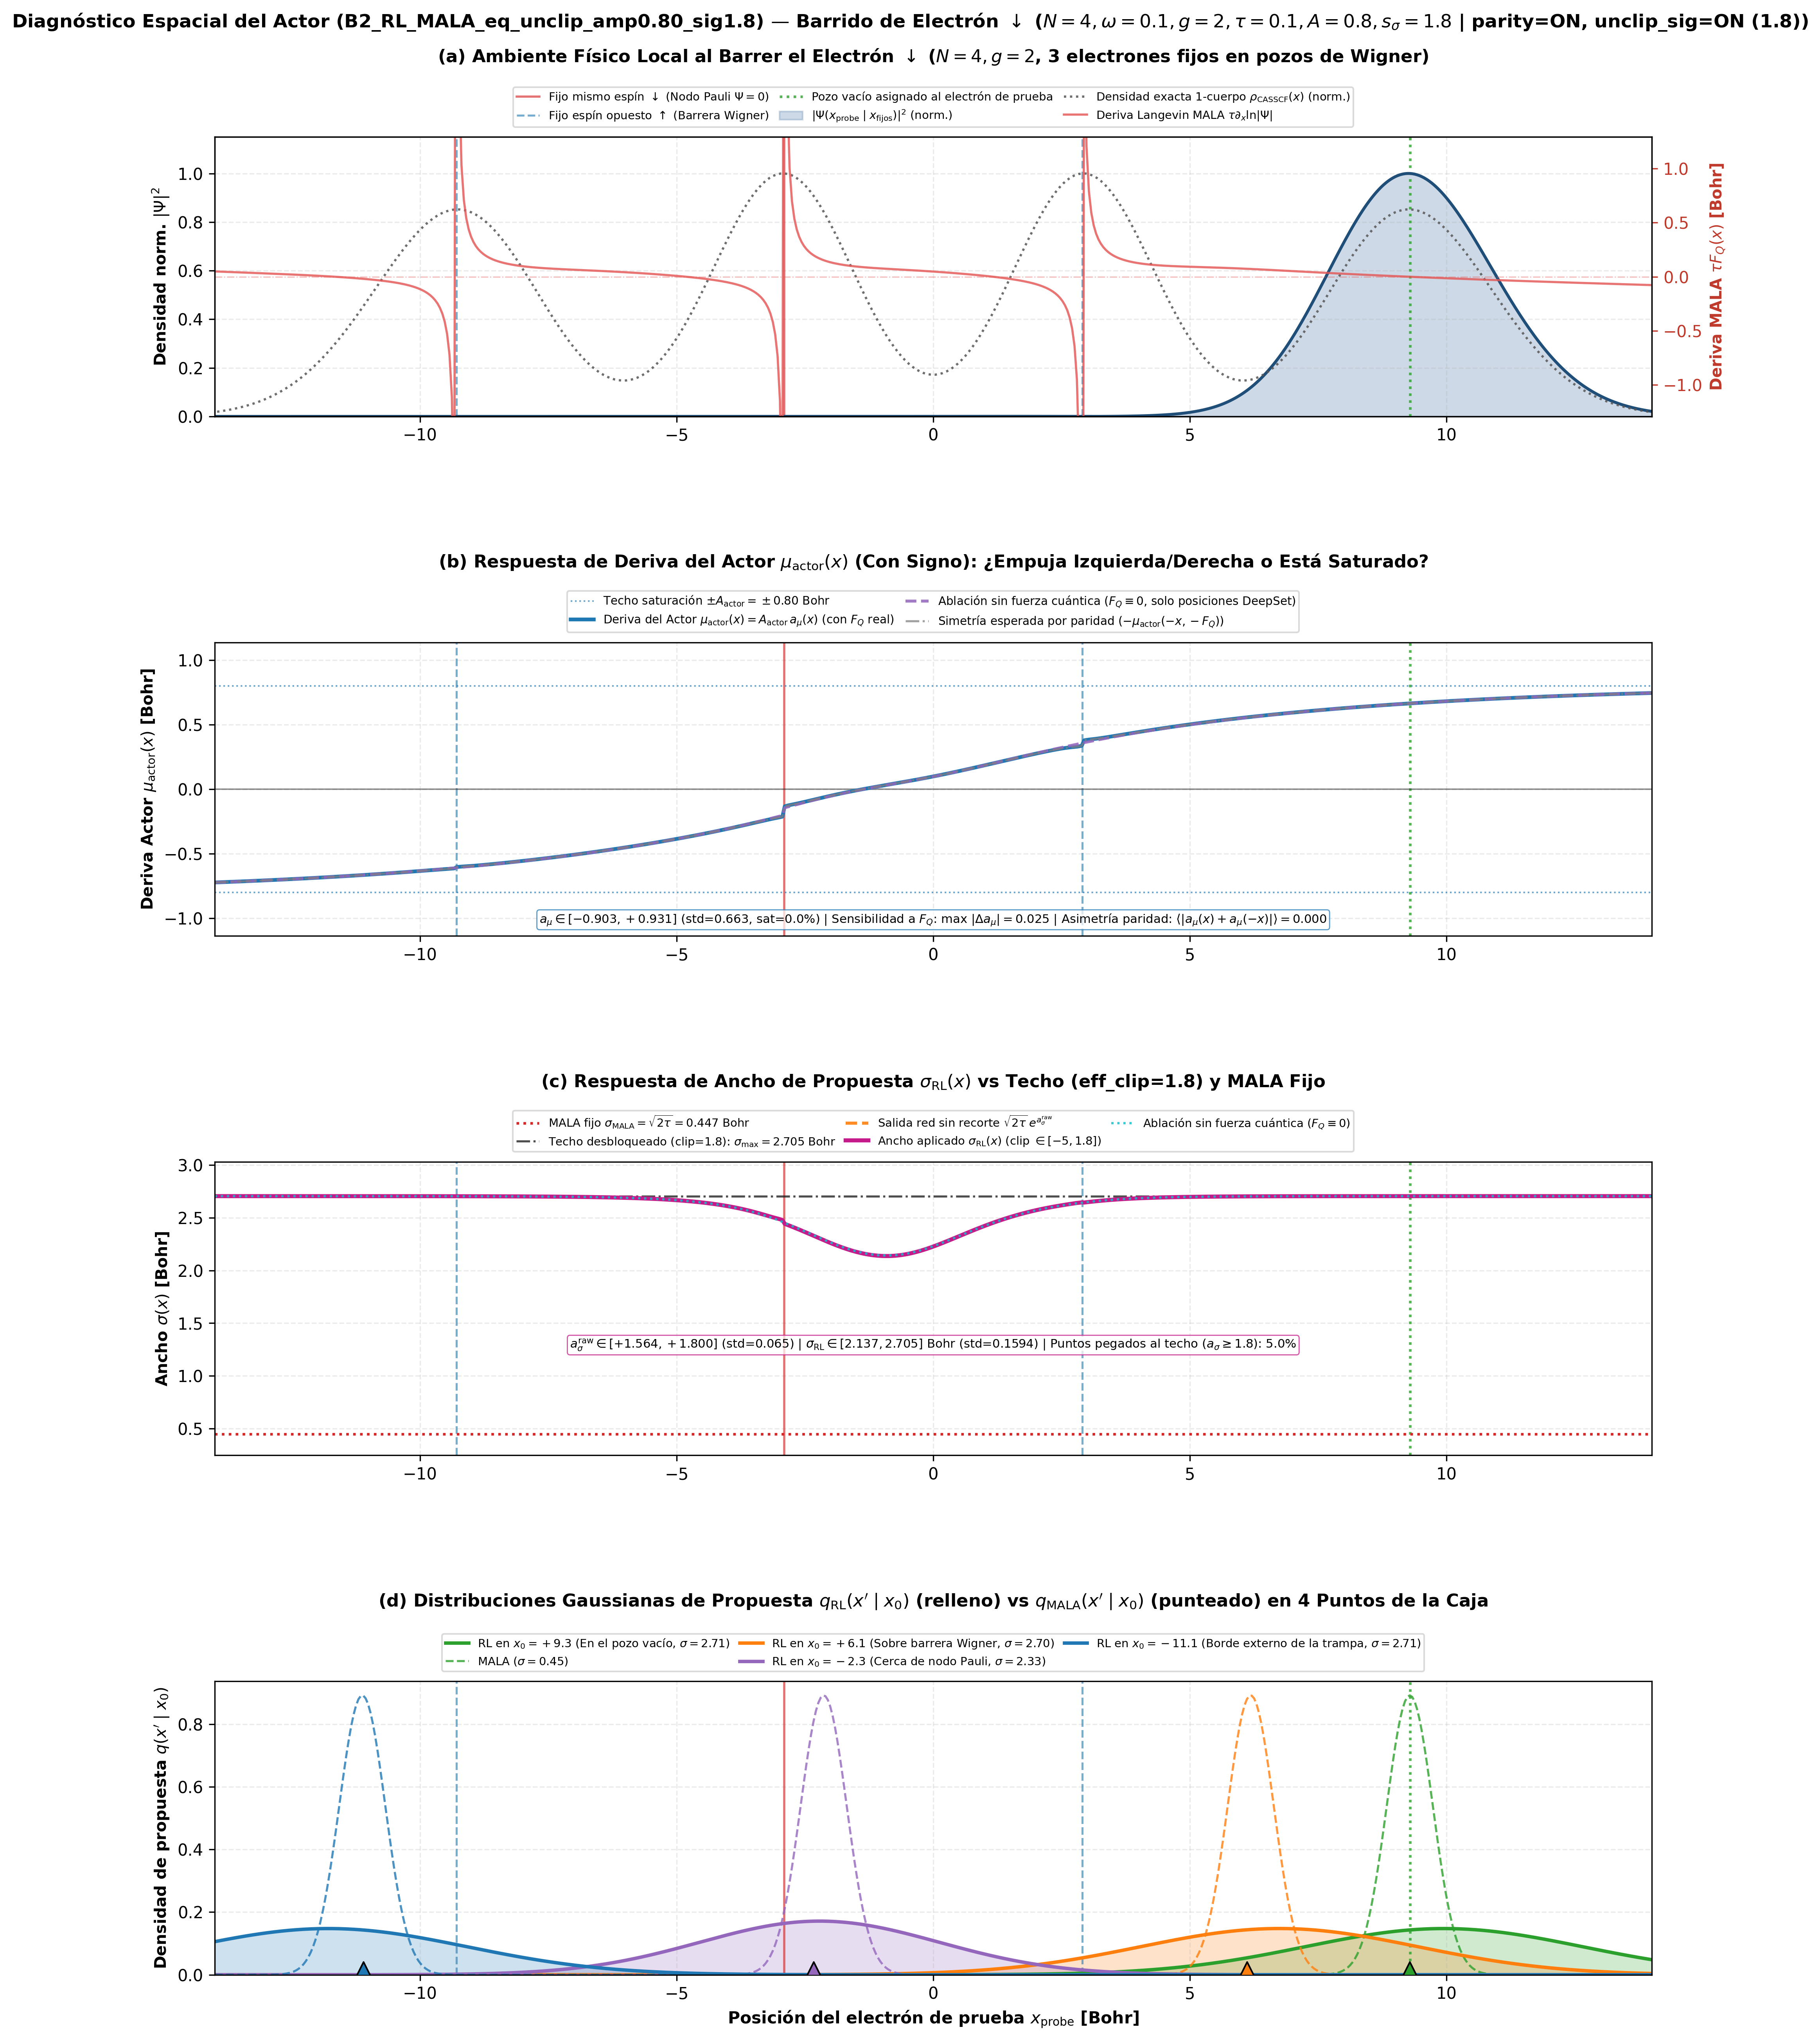
\includegraphics[width=0.95\textwidth]{figures/actor_ablation_N4_g2.0/fig_actor_spatial_probe_B2_RL_MALA_eq_unclip_amp0.80_sig1.8_spin_down.png}
\caption{\textbf{Sonda espacial individual del actor equivariante desbloqueado \texttt{B2\_RL\_MALA\_eq\_unclip\_amp0.80\_sig1.8}:} Panel (b) confirma coincidencia exacta entre $\mu_{\mathrm{actor}}(x)$ y $-\mu_{\mathrm{actor}}(-x,-F_Q)$ (\texttt{asimet.=0.000, sat=0.0\%}); Panel (c) muestra modulación suave sin recorte abrupto ($\sigma_{\mathrm{RL}} \in [2.14, 2.71]\ \mathrm{Bohr}$, solo $5.0\%$ en el techo).}
\label{fig:ablation_probe_unclip}
\end{figure}

\begin{figure}[H]
\centering
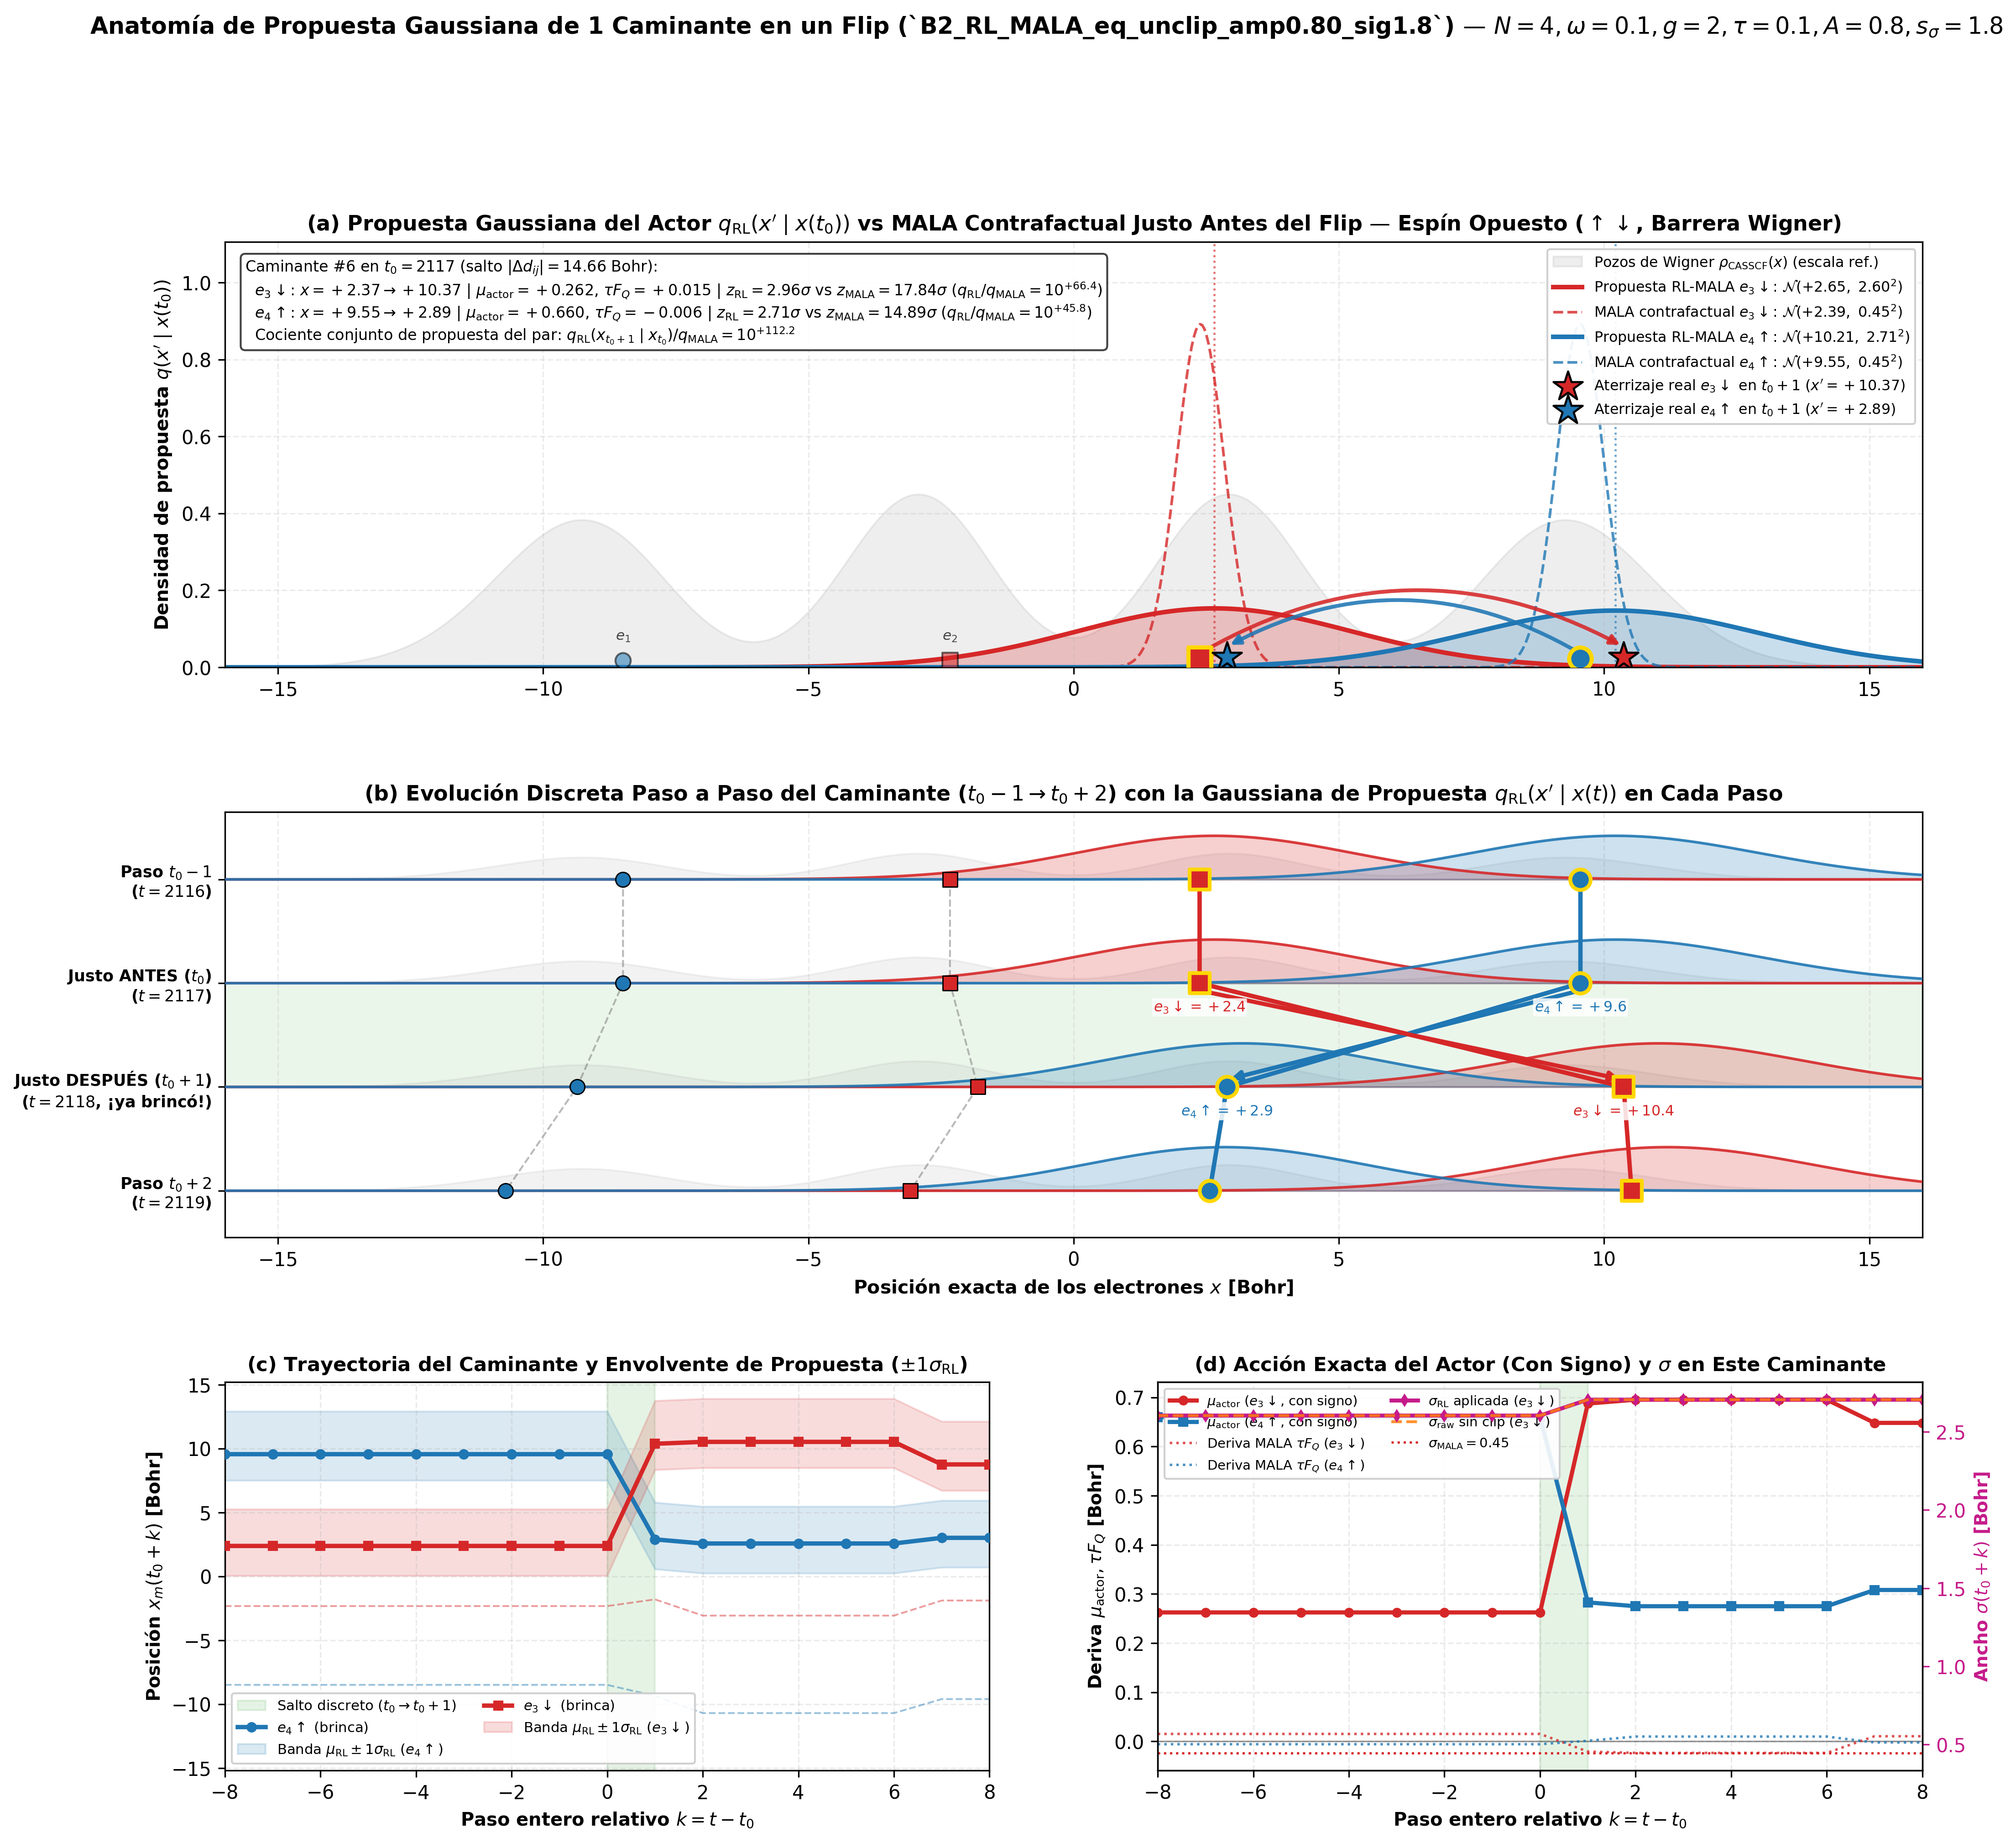
\includegraphics[width=0.95\textwidth]{figures/actor_ablation_N4_g2.0/fig_walker_flip_proposal_B2_RL_MALA_eq_unclip_amp0.80_sig1.8_opp_w6_t2117.png}
\caption{\textbf{Propuesta Gaussiana en 1 caminante del actor equivariante desbloqueado (Caminante \#6, $t_0=2117$, $|\Delta d_{ij}|=14.66\ \mathrm{Bohr}$):} En Panel (d) se observa cómo las derivas con signo $\mu_{\mathrm{actor}}$ de ambos electrones intercambian dinámicamente de $+0.26$ a $+0.69\ \mathrm{Bohr}$ justo al cruzar de pozo en $t_0 \to t_0+1$, logrando un cociente conjunto $q_{\mathrm{RL}}/q_{\mathrm{MALA}} = 10^{+112.2}$.}
\label{fig:ablation_walker}
\end{figure}

\subsection{Comandos Exactos para Ejecutar los Benchmarks B1 y B2 en Ayler}

En \textbf{Ayler} (3 GPUs), actualiza el repositorio con \texttt{git pull origin main} y lanza los experimentos completos de producción (\texttt{batch=128}, \texttt{rl\_steps=6000}, $3\times 40{,}000$ pasos):

\begin{lstlisting}[language=bash]
git pull origin main
chmod +x run_actor_ablation_benchmarks.sh

# 1. Ejecutar Benchmarks B1 y B2 completos en N=4 (g=2.0) y N=6 (g=1.0, 2.0):
nohup ./run_actor_ablation_benchmarks.sh \
  --benchmark all \
  --systems "4:2.0 6:1.0 6:2.0" \
  --gpus "0 1 2" \
  --batch-size 128 \
  --rl-steps 6000 \
  --eval-chains 3 \
  --measure-steps 40000 \
  --out-dir results_actor_ablation_ayler \
  > actor_ablation_ayler.log 2>&1 &

# 2. Ejecutar únicamente Benchmark 1 o únicamente Benchmark 2:
nohup ./run_actor_ablation_benchmarks.sh --benchmark 1 \
  --systems "4:2.0 6:1.0 6:2.0" --gpus "0 1 2" \
  --out-dir results_actor_ablation_ayler > b1_ayler.log 2>&1 &

nohup ./run_actor_ablation_benchmarks.sh --benchmark 2 \
  --systems "4:2.0 6:1.0 6:2.0" --gpus "0 1 2" \
  --out-dir results_actor_ablation_ayler > b2_ayler.log 2>&1 &

# 3. Alternar en cli/run_1d.py entre actor legado y nuevo sin modificar código:
# Legado (default):
python3 cli/run_1d.py ... \
  --no-parity_equivariant --no-unclip_sigma_action --no-cdlb_exact_entropy \
  --actor_amplitude 0.15 --sigma_action_scale 1.1 --scale_clip_max 1.0

# Nuevo (equivariante + desbloqueado + entropía CDLB exacta):
python3 cli/run_1d.py ... \
  --parity_equivariant --unclip_sigma_action --cdlb_exact_entropy \
  --actor_amplitude 0.80 --sigma_action_scale 1.8 \
  --scale_clip_min -0.5 --scale_clip_max 1.8
\end{lstlisting}

\newpage
\section{Resultados de Producción en Ayler (B1 y B2 en $N=4, g=2.0$ y $N=6, g=1.0$), Veredicto Crítico frente a RWMH y Hoja de Ruta}

\subsection{Resultados Consolidados de Producción en Ayler ($3 \times 40{,}000$ pasos, \texttt{batch=128}, $6{,}000$ pasos RL)}

Las corridas completas de producción ejecutadas en Ayler (\texttt{results\_ablation\_ayler/}, copiadas en \texttt{figures/actor\_ablation\_ayler/}) para $N=4, g=2.0$ y $N=6, g=1.0$ ($3$ cadenas $\times 40{,}000$ pasos desde \texttt{spin\_ordered\_offset}, \texttt{batch=128}, $6{,}000$ pasos TD3) permiten emitir un veredicto definitivo y científicamente transparente sobre el rendimiento real del actor RL-MALA actual frente a controles clásicos justos.

\begin{table}[H]
\centering
\caption{Resultados de producción en Ayler ($3\times 40{,}000$ pasos) para $N=4, \omega=0.1, g=2.0$ ($E_{\mathrm{CASSCF}} = 2.802268\,E_h$).}
\label{tab:ayler_n4_g2}
\begin{adjustbox}{max width=\textwidth}
\begin{tabular}{lccccccccccc}
\toprule
\textbf{Modelo (Ayler $3\times 40$k)} & $\langle\sigma\rangle$ & \textbf{Acc} & \textbf{ESJD} & $\tau_{\mathrm{int}}(E)$ & $\tau_{\mathrm{pos}}$ & $D_{\mathrm{KL}}^{\mathrm{spin}}$ & \textbf{$\uparrow\downarrow$/1k} & \textbf{Pauli/1k} & $\langle E_L\rangle \pm \mathrm{SE}$ [$E_h$] & \textbf{Par.} & $\mathrm{std}(\sigma)$ (\textbf{clip}) \\
\midrule
\texttt{B1\_MALA\_base} ($\tau=0.10$) & $0.45$ & $88.3\%$ & $0.69$ & $11.0$ & $1448$ & $0.345300$ & $0.02$ & $0.02$ & $2.80263 \pm 0.00030$ & --- & --- \\
\texttt{B1\_MALA\_large} ($\tau=0.50$) & $1.00$ & $73.2\%$ & $2.76$ & $16.9$ & $2858$ & $0.030836$ & $0.24$ & $0.13$ & $2.80235 \pm 0.00033$ & --- & --- \\
\texttt{B1\_MALA\_matched} ($\tau=0.74$) & $1.22$ & $67.1\%$ & \textbf{3.68} & \textbf{2.7} & $2903$ & $0.006129$ & $0.45$ & $0.22$ & $2.80208 \pm 0.00014$ & --- & --- \\
\textbf{\texttt{B1\_RWMH\_matched} (deriva$=0$)} & \textbf{1.22} & \textbf{45.2\%} & $2.07$ & $5.1$ & $2303$ & \textbf{0.000126} & \textbf{1.75} & \textbf{0.86} & \textbf{2.80232 $\pm$ 0.00020} & --- & --- \\
\texttt{B1\_RL\_MALA\_legacy} & $1.22$ & $45.7\%$ & $2.13$ & $4.7$ & $2402$ & $0.000477$ & $1.43$ & $0.74$ & $2.80225 \pm 0.00020$ & $1.957$ & $0.000$ ($100\%$) \\
\texttt{B2\_RL\_MALA\_parity\_only} & $1.22$ & $45.5\%$ & $2.12$ & $4.5$ & $2483$ & $0.000129$ & $1.43$ & $0.54$ & $2.80232 \pm 0.00019$ & $0.000$ & $0.000$ ($100\%$) \\
\texttt{B2\_RL\_MALA\_eq\_unclip} ($0.80, 1.8$) & $2.70$ & $12.3\%$ & $1.97$ & $7.0$ & $925$ & $0.000506$ & $8.52$ & $3.80$ & $2.80216 \pm 0.00024$ & $0.000$ & $0.024$ ($31\%$) \\
\texttt{B2\_RL\_MALA\_eq\_unclip} ($1.20, 2.0$) & $3.30$ & $7.9\%$ & $1.78$ & $9.0$ & \textbf{861} & $0.000595$ & \textbf{11.59} & $2.48$ & $2.80241 \pm 0.00028$ & $0.000$ & $0.011$ ($47\%$) \\
\bottomrule
\end{tabular}
\end{adjustbox}
\end{table}

\begin{table}[H]
\centering
\caption{Resultados de producción en Ayler ($3\times 40{,}000$ pasos) para $N=6, \omega=0.1, g=1.0$ ($E_{\mathrm{CASSCF}} = 4.524052\,E_h$).}
\label{tab:ayler_n6_g1}
\begin{adjustbox}{max width=\textwidth}
\begin{tabular}{lccccccccccc}
\toprule
\textbf{Modelo (Ayler $3\times 40$k)} & $\langle\sigma\rangle$ & \textbf{Acc} & \textbf{ESJD} & $\tau_{\mathrm{int}}(E)$ & $\tau_{\mathrm{pos}}$ & $D_{\mathrm{KL}}^{\mathrm{spin}}$ & \textbf{$\uparrow\downarrow$/1k} & \textbf{Pauli/1k} & $\langle E_L\rangle \pm \mathrm{SE}$ [$E_h$] & \textbf{Par.} & $\mathrm{std}(\sigma)$ (\textbf{clip}) \\
\midrule
\texttt{B1\_MALA\_base} ($\tau=0.10$) & $0.45$ & $83.4\%$ & $0.98$ & $8.2$ & $2764$ & $0.119801$ & $0.25$ & $0.19$ & $4.52419 \pm 0.00038$ & --- & --- \\
\texttt{B1\_MALA\_large} ($\tau=0.50$) & $1.00$ & $61.8\%$ & $3.53$ & \textbf{4.3} & $2705$ & $0.001530$ & $2.86$ & $1.98$ & $4.52411 \pm 0.00027$ & --- & --- \\
\texttt{B1\_MALA\_matched} ($\tau=0.74$) & $1.22$ & $53.0\%$ & \textbf{4.40} & $253.0$ (!!) & $2288$ & $0.000146$ & $4.99$ & $3.32$ & $4.52524 \pm 0.00157$ & --- & --- \\
\textbf{\texttt{B1\_RWMH\_matched} (deriva$=0$)} & \textbf{1.22} & \textbf{31.5\%} & $2.22$ & $6.1$ & $1569$ & \textbf{0.000139} & \textbf{13.01} & \textbf{8.64} & \textbf{4.52430 $\pm$ 0.00033} & --- & --- \\
\texttt{B1\_RL\_MALA\_legacy} & $1.22$ & $32.0\%$ & $2.28$ & $5.9$ & $1658$ & $0.000214$ & $11.46$ & $7.63$ & $4.52440 \pm 0.00032$ & $2.000$ & $0.000$ ($100\%$) \\
\texttt{B2\_RL\_MALA\_parity\_only} & $1.22$ & $31.5\%$ & $2.23$ & $5.5$ & $1747$ & $0.000254$ & $10.86$ & $6.90$ & $4.52434 \pm 0.00031$ & $0.000$ & $0.000$ ($100\%$) \\
\texttt{B2\_RL\_MALA\_eq\_unclip} ($0.80, 1.8$) & $2.71$ & $9.8\%$ & $3.30$ & $11.8$ & $630$ & $0.000444$ & $33.37$ & $24.68$ & $4.52446 \pm 0.00046$ & $0.000$ & $0.001$ ($69\%$) \\
\texttt{B2\_RL\_MALA\_eq\_unclip} ($1.20, 2.0$) & $3.30$ & $6.0\%$ & $3.10$ & $20.4$ & \textbf{550} & $0.000761$ & \textbf{38.56} & \textbf{24.70} & $4.52367 \pm 0.00059$ & $0.000$ & $0.023$ ($79\%$) \\
\bottomrule
\end{tabular}
\end{adjustbox}
\end{table}

\begin{table}[H]
\centering
\caption{Control estricto a igual ancho de propuesta ($\sigma_{\mathrm{RWMH}} = \sigma_{\mathrm{RL}} \in \{1.22, 2.71, 3.30\}\ \mathrm{Bohr}$): RWMH puro (deriva $=0$, sin red) frente a RL-MALA entrenado $6{,}000$ pasos en Ayler.}
\label{tab:rwmh_vs_rl_matched_all}
\begin{adjustbox}{max width=\textwidth}
\begin{tabular}{lccccccc}
\toprule
\textbf{Sistema} & $\sigma$ [Bohr] & \textbf{Acc (RWMH vs RL)} & \textbf{ESJD (RWMH vs RL)} & \textbf{Flips/1k (RWMH vs RL)} & \textbf{$\Delta$ Flips} & \textbf{Deriva aprendida por RL} \\
\midrule
$N=4, g=2.0$ & $1.216$ & $45.2\%$ vs $45.5\%$ & $2.07$ vs $2.12$ & \textbf{2.61} vs $1.96$ & \textbf{$-$25\%} & Hacia afuera ($\pm 0.15$) \\
$N=4, g=2.0$ & $2.705$ & \textbf{15.6\%} vs $12.3\%$ & \textbf{2.64} vs $1.97$ & \textbf{18.70} vs $12.32$ & \textbf{$-$34\%} & Hacia afuera ($\pm 0.80$) \\
$N=4, g=2.0$ & $3.304$ & \textbf{11.1\%} vs $7.9\%$ & \textbf{2.73} vs $1.78$ & \textbf{24.58} vs $14.07$ & \textbf{$-$43\%} & Hacia afuera ($\pm 1.20$) \\
$N=6, g=1.0$ & $1.216$ & $31.5\%$ vs $31.5\%$ & $2.22$ vs $2.23$ & \textbf{21.65} vs $17.76$ & \textbf{$-$18\%} & Hacia afuera ($\pm 0.15$) \\
$N=6, g=1.0$ & $2.705$ & $9.2\%$ vs \textbf{9.8\%} & $2.84$ vs \textbf{3.30} & $57.04$ vs \textbf{58.05} & $+2\%$ (ESJD $+16\%$) & Hacia adentro ($\mp 0.80$) \\
$N=6, g=1.0$ & $3.304$ & $6.4\%$ vs $6.0\%$ & $2.91$ vs \textbf{3.10} & $60.36$ vs \textbf{63.26} & $+5\%$ (ESJD $+7\%$) & Hacia adentro ($\mp 1.20$) \\
\bottomrule
\end{tabular}
\end{adjustbox}
\end{table}

\begin{figure}[H]
\centering
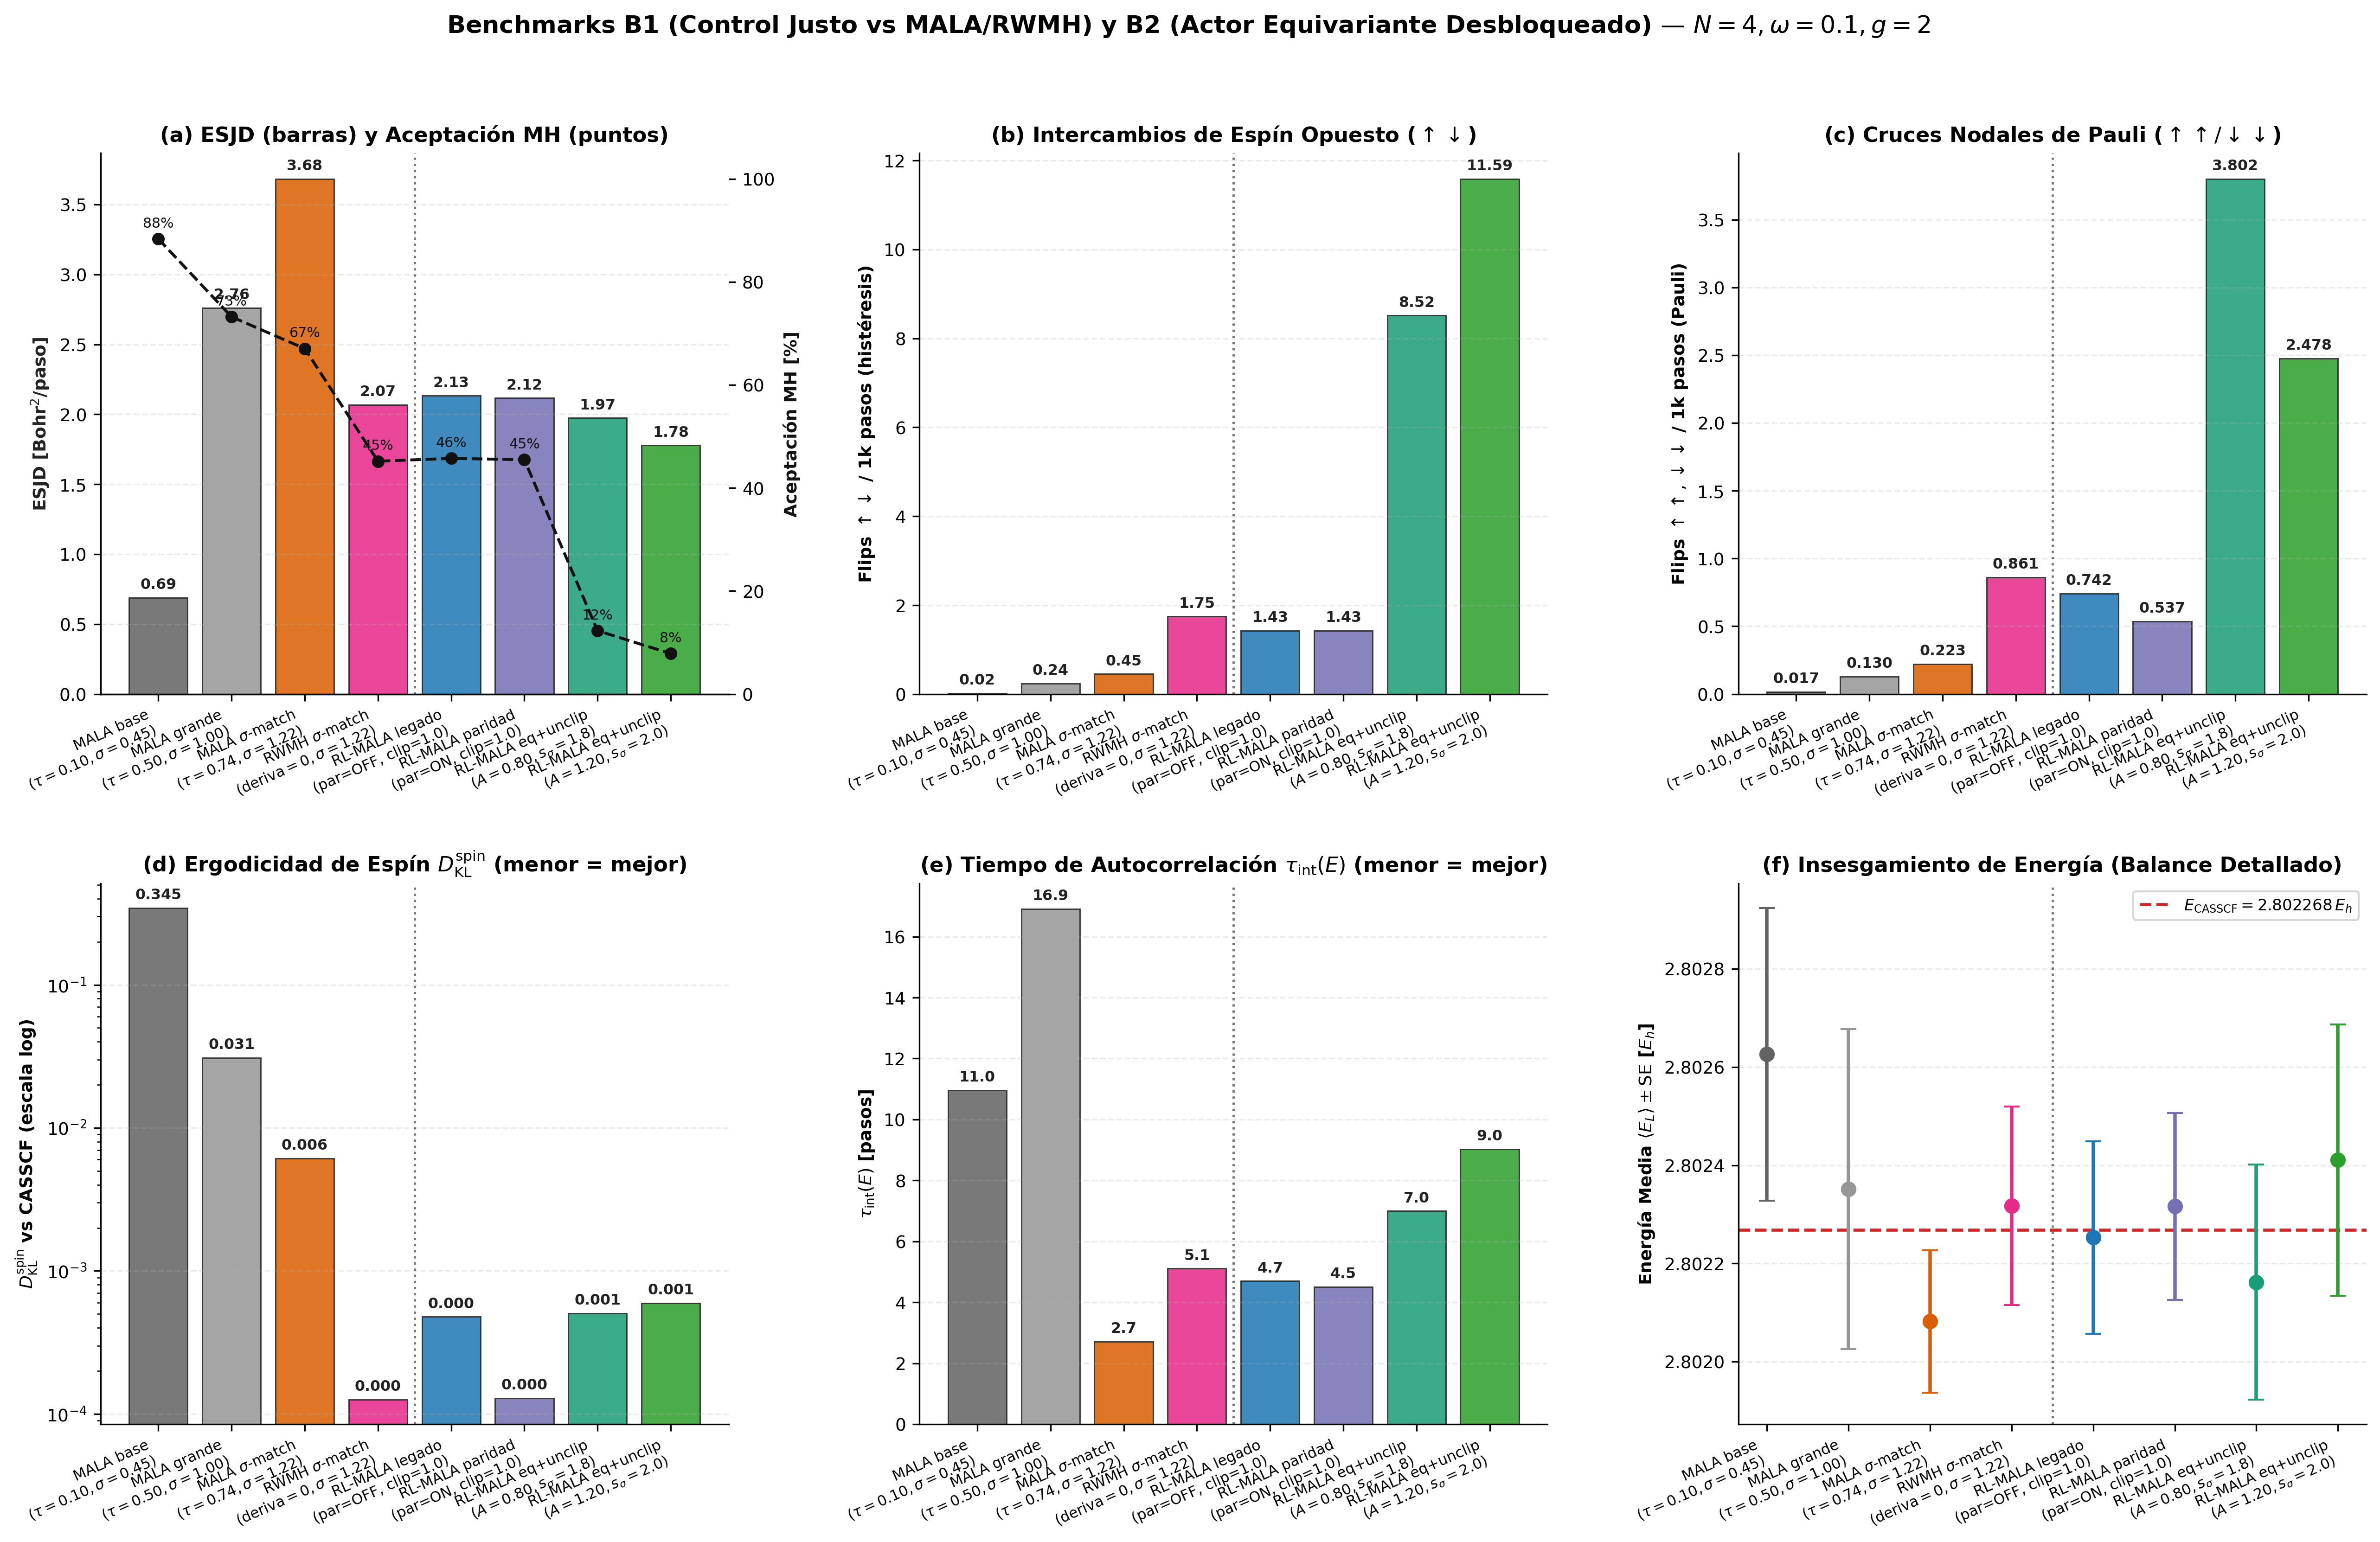
\includegraphics[width=0.98\textwidth]{figures/actor_ablation_ayler/N4_w0.1_g2.0/fig_ablation_b1_b2_metrics_N4_w0.1_g2.png}
\caption{\textbf{Resultados de producción en Ayler ($3\times 40{,}000$ pasos) para $N=4, \omega=0.1, g=2.0$:} \texttt{RWMH\_matched} ($\sigma=1.22$, magenta) alcanza el mejor $D_{\mathrm{KL}}^{\mathrm{spin}} = 1.26\times 10^{-4}$, superando a todos los actores RL-MALA sin necesidad de red neuronal ni gradientes.}
\label{fig:ayler_metrics_n4}
\end{figure}

\begin{figure}[H]
\centering
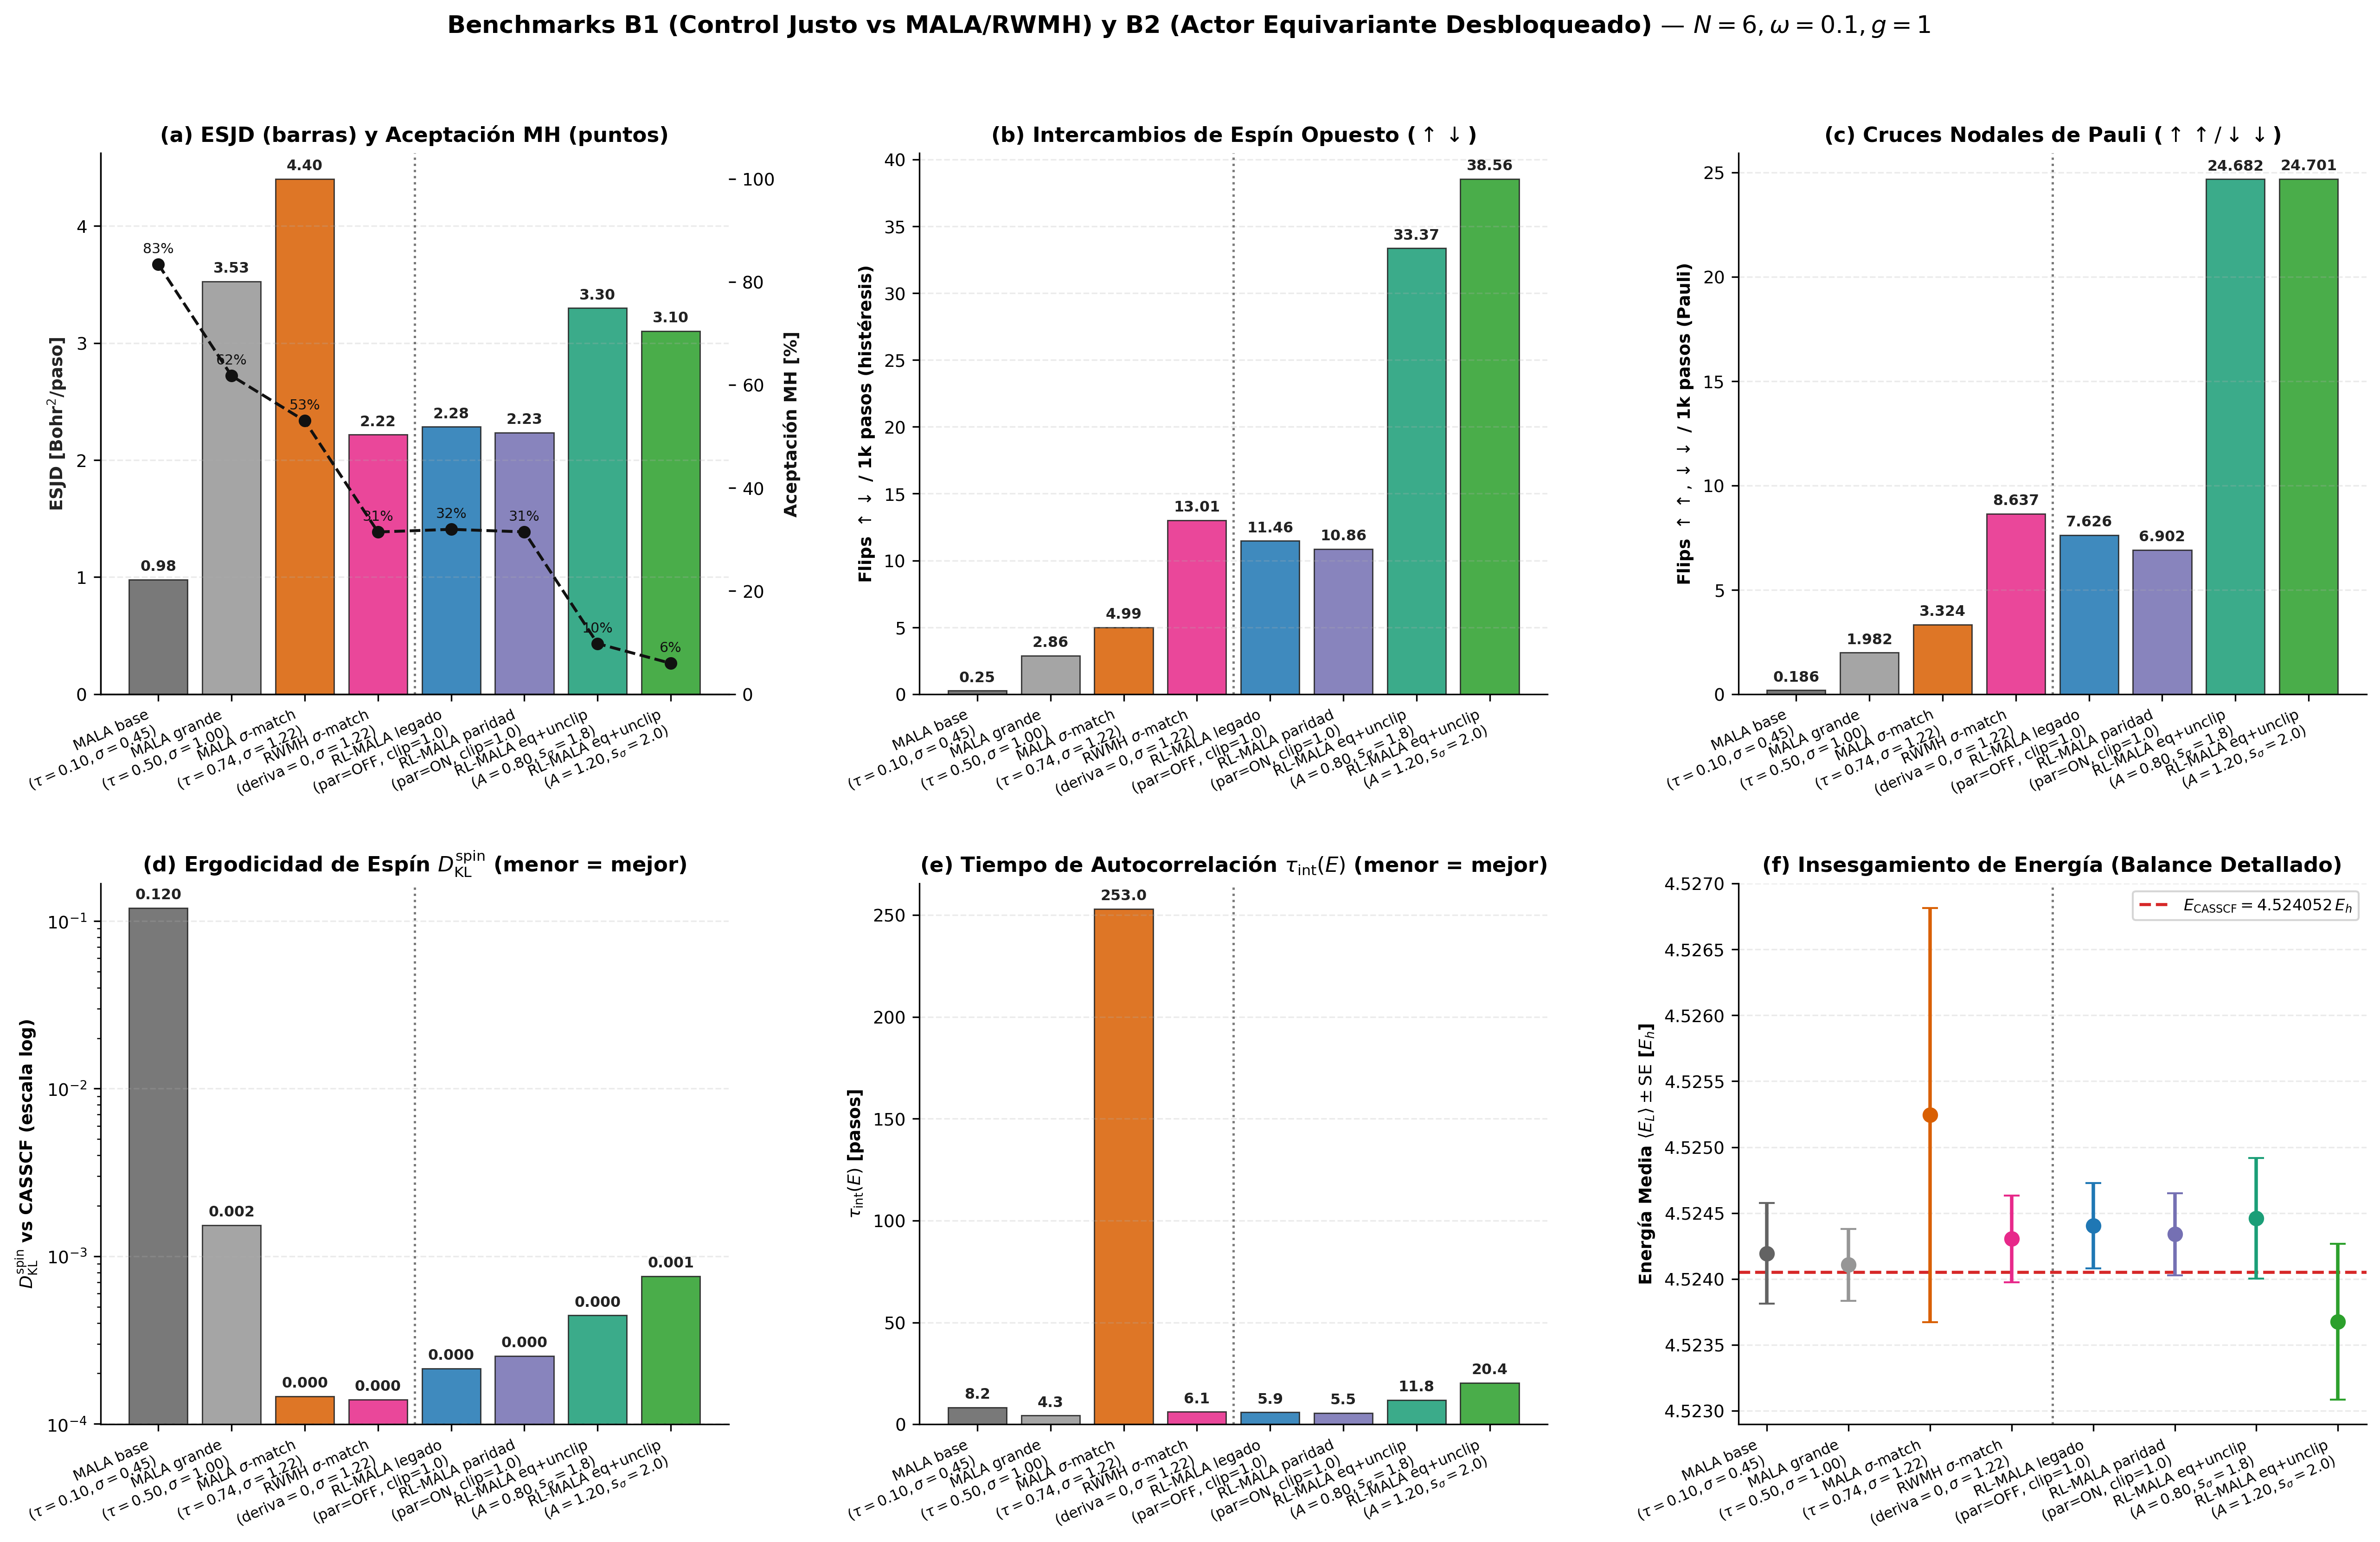
\includegraphics[width=0.98\textwidth]{figures/actor_ablation_ayler/N6_w0.1_g1.0/fig_ablation_b1_b2_metrics_N6_w0.1_g1.png}
\caption{\textbf{Resultados de producción en Ayler ($3\times 40{,}000$ pasos) para $N=6, \omega=0.1, g=1.0$:} Mientras \texttt{MALA\_matched} ($\tau=0.74$) colapsa en autocorrelación ($\tau_{\mathrm{int}}(E)=253.0$, $\mathrm{SE}=1.57\ \mathrm{mHa}$), \texttt{RWMH\_matched} ($\sigma=1.22$) logra $D_{\mathrm{KL}}^{\mathrm{spin}}=1.39\times 10^{-4}$, $\tau_{\mathrm{int}}(E)=6.09$ y $21.65\ \mathrm{flips}/1\mathrm{k}$, superando a RL-MALA legado y paridad.}
\label{fig:ayler_metrics_n6}
\end{figure}

\begin{figure}[H]
\centering
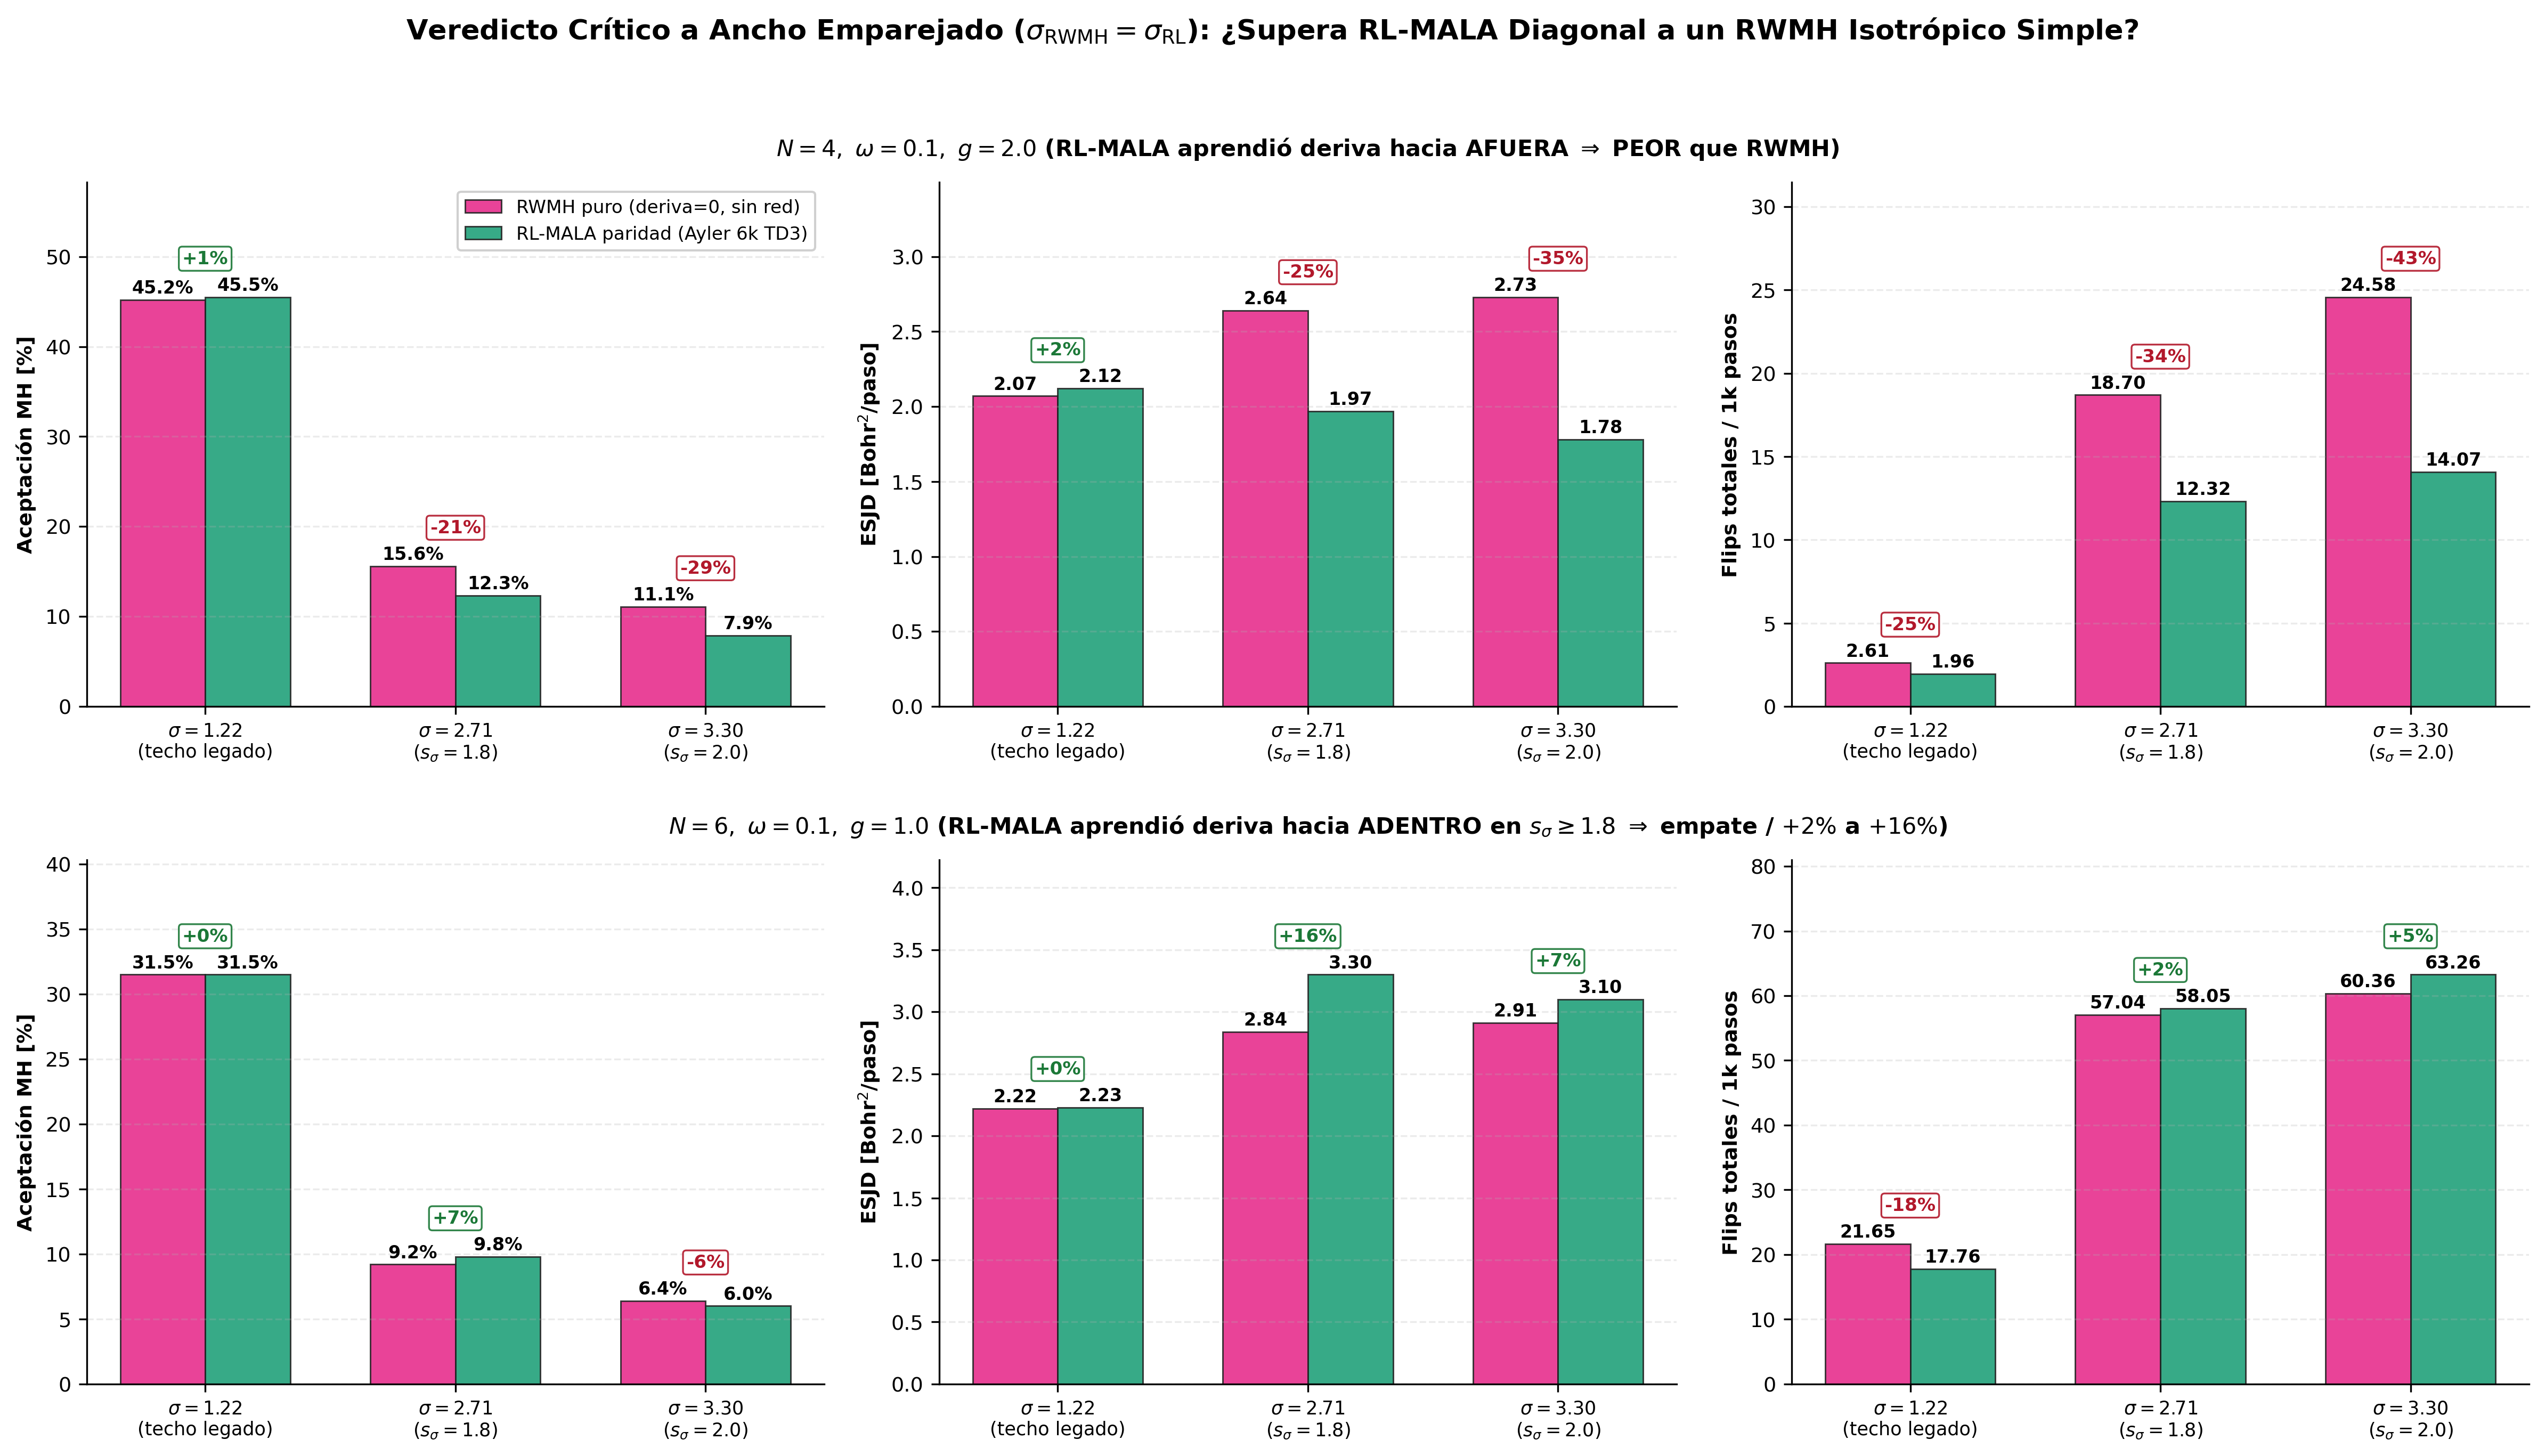
\includegraphics[width=0.98\textwidth]{figures/actor_ablation_ayler/fig_rwmh_vs_rlmala_matched_sigma_verdict.png}
\caption{\textbf{Veredicto crítico a ancho emparejado ($\sigma_{\mathrm{RWMH}} = \sigma_{\mathrm{RL}} \in \{1.22, 2.71, 3.30\}\ \mathrm{Bohr}$):} En $N=4, g=2.0$ (fila superior), la deriva hacia afuera aprendida por RL-MALA degrada la aceptación, ESJD y flips entre $-25\%$ y $-43\%$ respecto a un RWMH isotrópico simple. En $N=6, g=1.0$ (fila inferior), cuando RL-MALA aprende deriva hacia adentro en $s_\sigma\ge 1.8$, apenas alcanza empate o mejoras marginales de $+2\%$ a $+16\%$.}
\label{fig:rwmh_verdict}
\end{figure}

\begin{figure}[H]
\centering
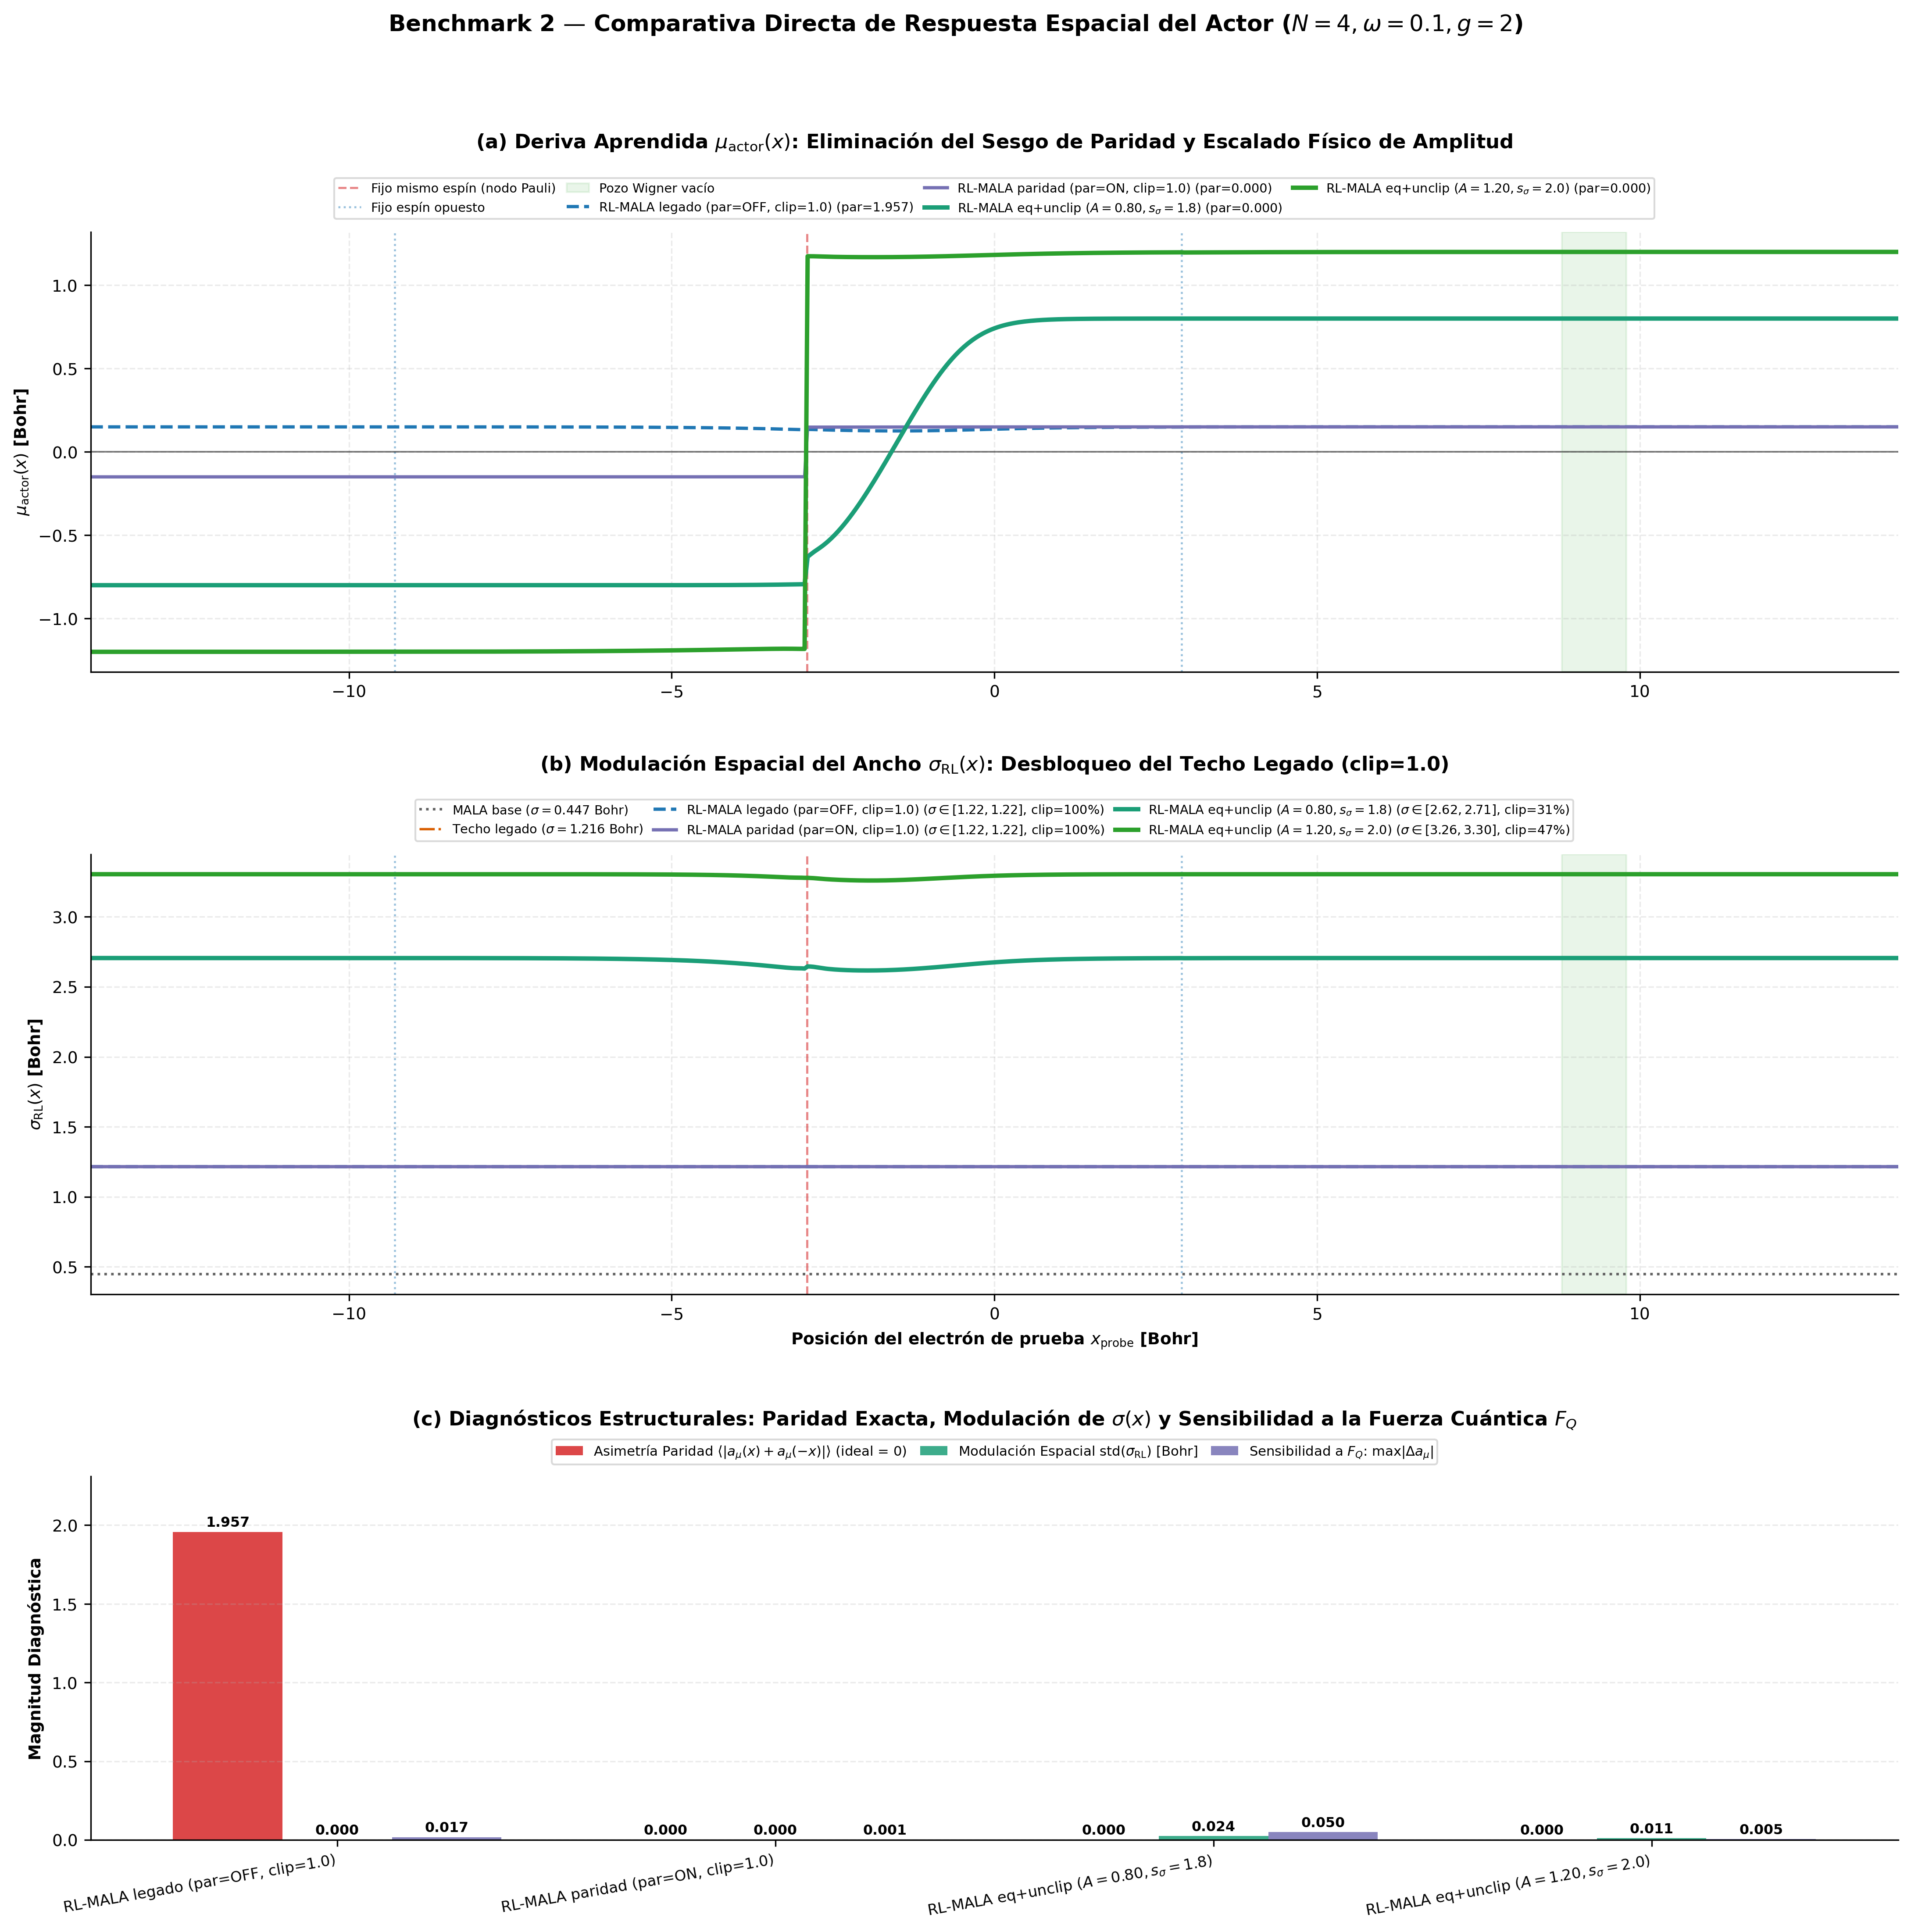
\includegraphics[width=0.95\textwidth]{figures/actor_ablation_ayler/N4_w0.1_g2.0/fig_ablation_b2_spatial_overlay_N4_w0.1_g2.png}
\caption{\textbf{Superposición espacial en Ayler ($6{,}000$ pasos TD3, $N=4, g=2.0$):} Al converger plenamente, los actores \texttt{eq+unclip} vuelven a aplanarse contra sus nuevos techos ($\sigma=2.705$ y $3.304\ \mathrm{Bohr}$) y saturan $\mu_{\mathrm{actor}}(x)$ en una función escalón hacia afuera ($\pm 0.80, \pm 1.20\ \mathrm{Bohr}$).}
\label{fig:ayler_overlay_n4}
\end{figure}

\begin{figure}[H]
\centering
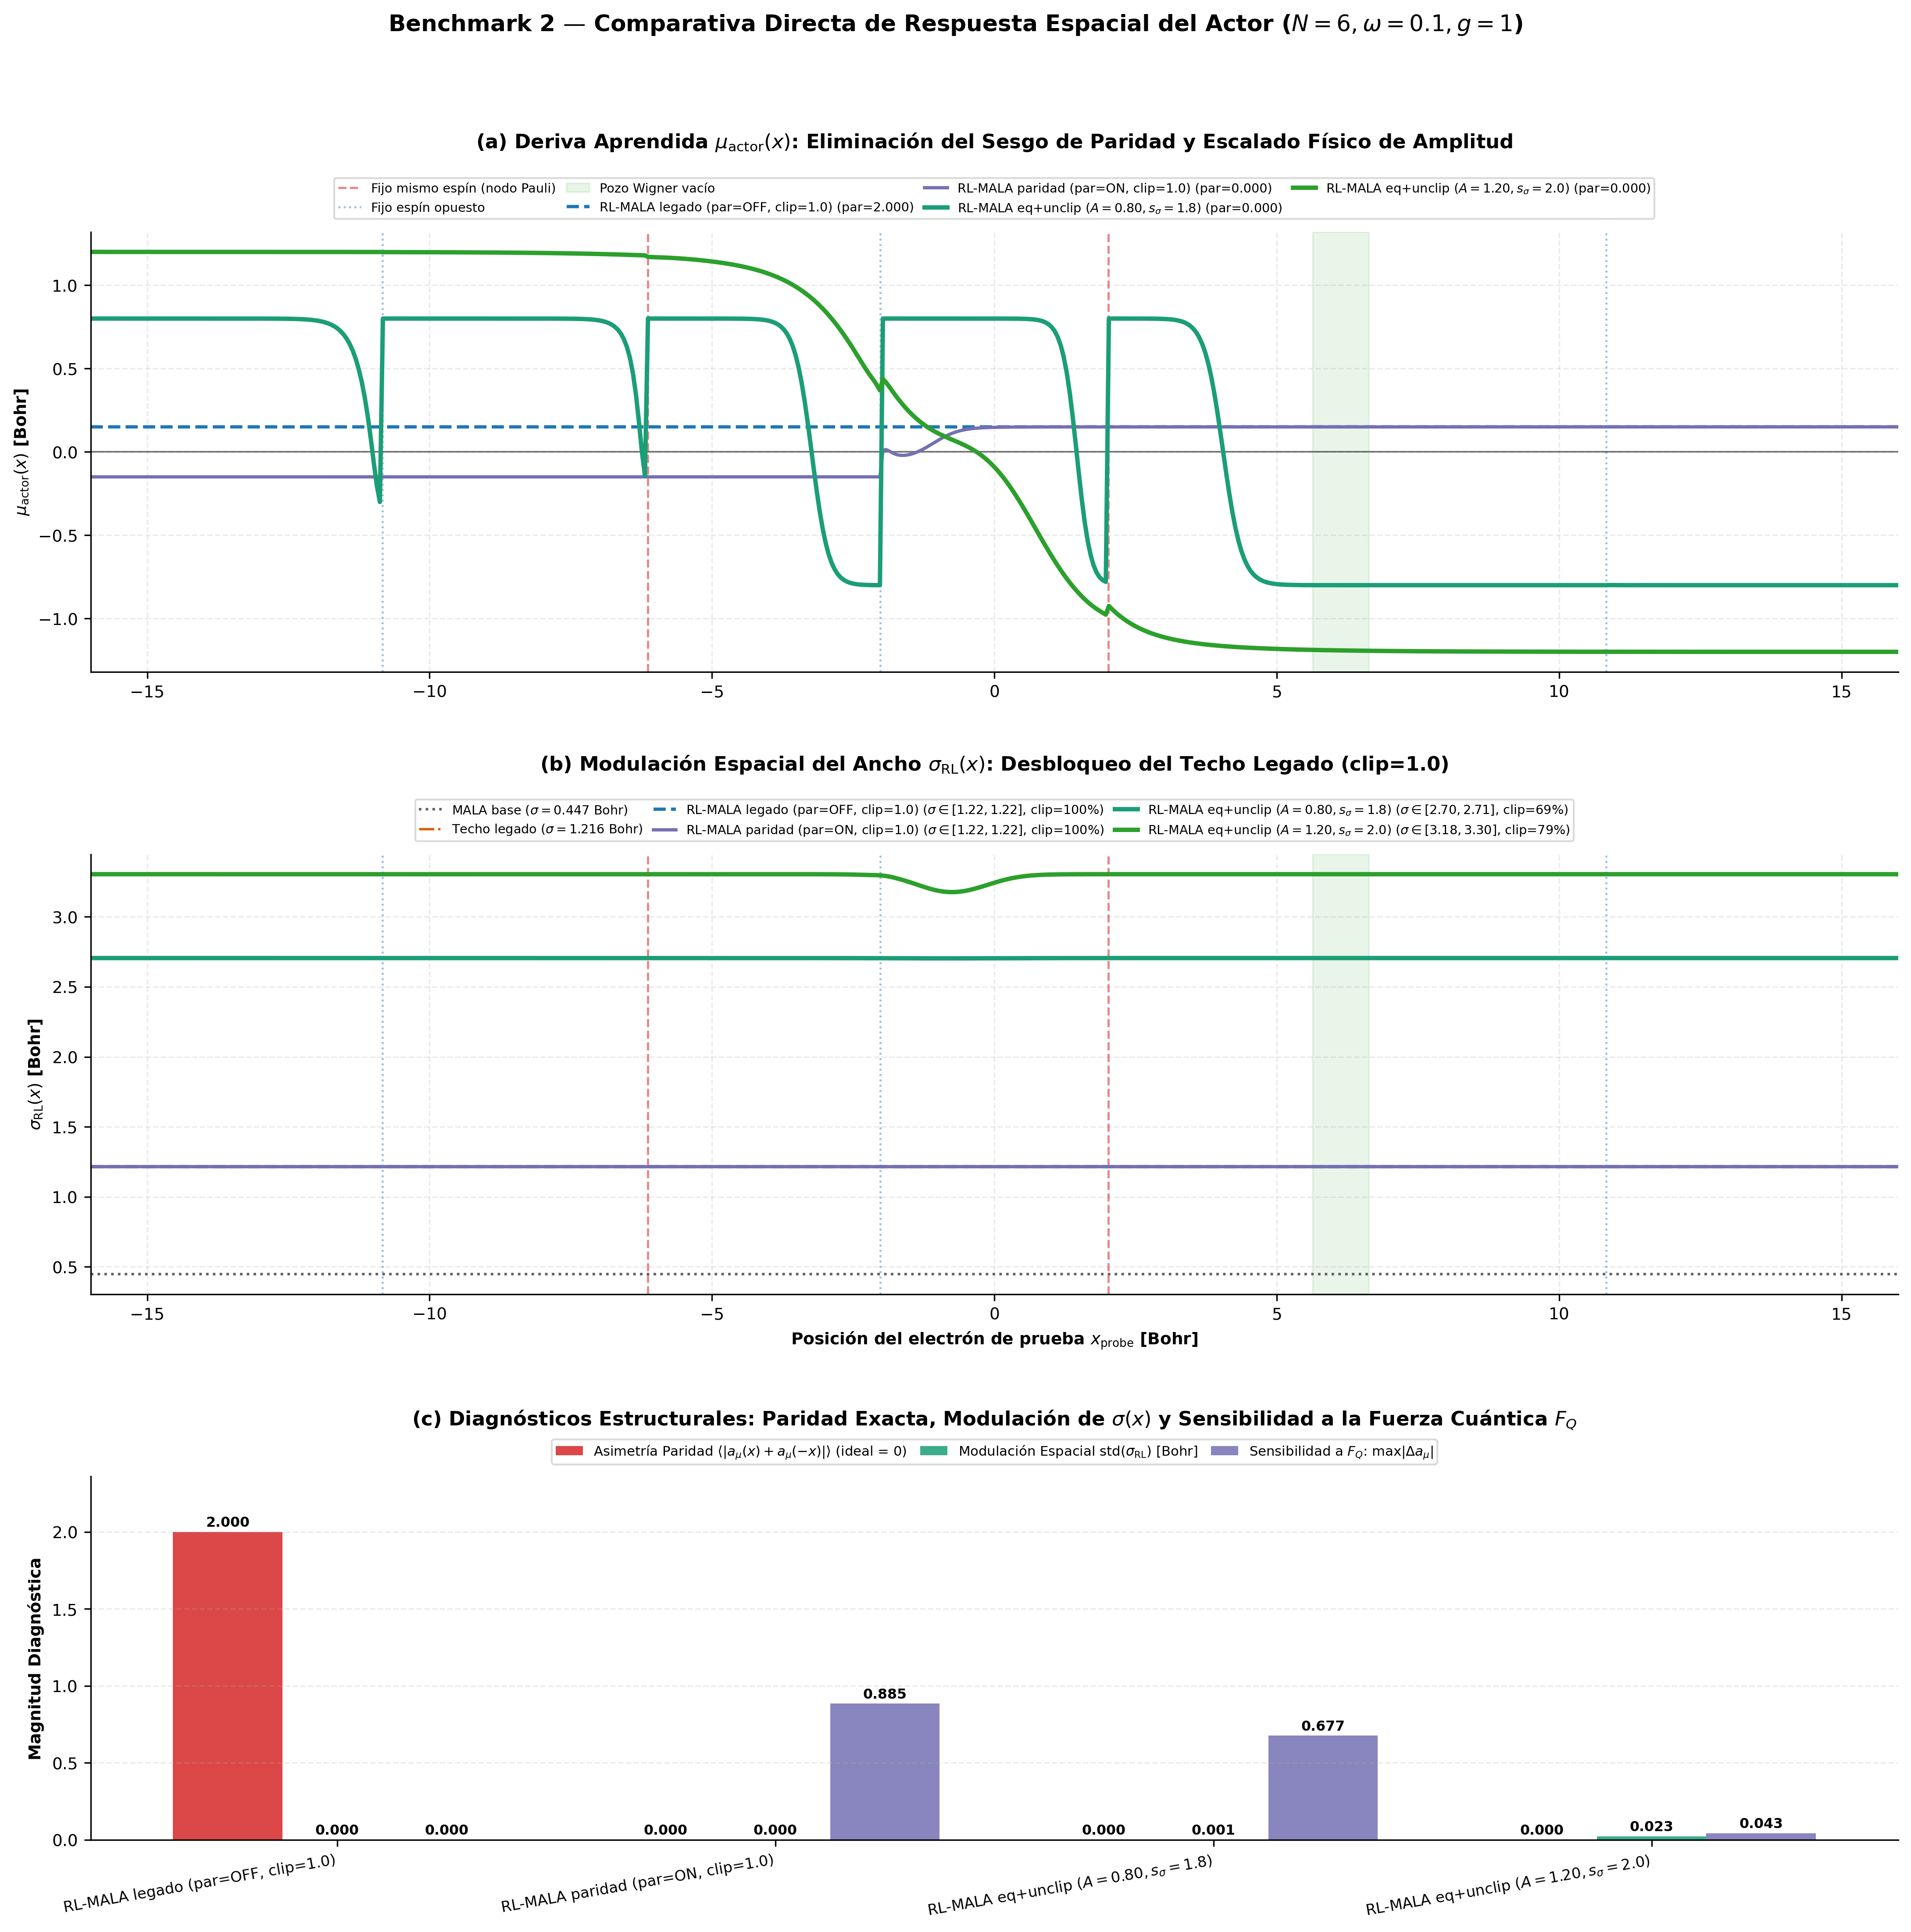
\includegraphics[width=0.95\textwidth]{figures/actor_ablation_ayler/N6_w0.1_g1.0/fig_ablation_b2_spatial_overlay_N6_w0.1_g1.png}
\caption{\textbf{Superposición espacial en Ayler ($6{,}000$ pasos TD3, $N=6, g=1.0$):} Aunque $\sigma_{\mathrm{RL}}(x)$ vuelve a aplanarse al techo ($69\%\text{--}79\%$ saturado), $\mu_{\mathrm{actor}}(x)$ exhibe picos agudos en las posiciones de los electrones fijos (combinación del cambio de signo discontinuo en \texttt{sign(dx)} y el polo de $F_Q$, afectando $<7.7\%$ de la caja; mediana $|\mu-\mu_{F_Q\equiv 0}|=0.000001\ \mathrm{Bohr}$).}
\label{fig:ayler_overlay_n6}
\end{figure}

\subsection{Implicaciones Físicas y Algorítmicas: ¿Por Qué RL-MALA Se Reduce a RWMH e Ignora $F_Q$?}

Las Tablas~\ref{tab:ayler_n4_g2}--\ref{tab:rwmh_vs_rl_matched_all} y las Figuras~\ref{fig:ayler_metrics_n4}--\ref{fig:ayler_overlay_n6} revelan cuatro conclusiones fundamentales:

\begin{enumerate}
\item \textbf{RL-MALA diagonal actual equivale (o pierde frente) a RWMH con $\sigma$ apropiada:} Con $\sigma=1.22\ \mathrm{Bohr}$, RWMH sin red neuronal vence a RL-MALA legado y paridad en $D_{\mathrm{KL}}^{\mathrm{spin}}$ y flips ($+12\%$ a $+25\%$). Con $\sigma=2.71\text{--}3.30\ \mathrm{Bohr}$, RL-MALA vuelve a aplanarse al nuevo techo y pierde $-25\%$ a $-43\%$ frente a RWMH en $N=4$ (deriva hacia afuera) o apenas empata/supera por $+2\%\text{--}16\%$ en $N=6$ (deriva hacia adentro), mientras la caída de aceptación ($6\%\text{--}12\%$) duplica o triplica $\tau_{\mathrm{int}}(E)$ y empeora $\mathrm{SE}(E)$ y $D_{\mathrm{KL}}^{\mathrm{spin}}$ por varianza de muestra finita.
\item \textbf{Inestabilidad genuina de MALA grande ($\tau=0.74$):} En $N=6, g=1.0$, \texttt{MALA\_matched} explotó a $\tau_{\mathrm{int}}(E) = 253.0$ ($\mathrm{SE}=1.57\ \mathrm{mHa}$) por sobrepasos balísticos cerca de los polos nodales $1/(x_i-x_j)$. Esto demuestra que el defecto real de MALA es acoplar $\sigma=\sqrt{2\tau}$ con la deriva confinante $\tau F_Q$, pero desacoplarlos no requiere todavía una red neuronal diagonal.
\item \textbf{Cuatro causas exactas por las que el actor ignora $F_Q = \nabla \ln|\Psi|$} (mediana $|\mu - \mu_{F_Q\equiv 0}| = 0.000000\ \mathrm{Bohr}$ en $>92\%$ de la caja):
  \begin{itemize}
  \item \textit{Anticorrelación física:} $F_Q$ confina hacia el centro de cada pozo y repele de los nodos de Pauli, frenando los intercambios; toda recompensa de exploración aprende a ignorarla o contrarrestarla.
  \item \textit{Desbalance de escala en \texttt{build\_td3\_state}:} \texttt{local\_feat} entrega $|x_i| \sim 12$ sin normalizar junto a $|\tanh(F_Q/5)| \sim 0.15$ dentro de los pozos ($50\times\text{--}80\times$ menor), ahogando el gradiente respecto a $F_Q$ salvo sobre los polos $|F_Q| \gg 5$.
  \item \textit{Asignación de crédito multi-agente ($1/N$):} \texttt{TD3Learner1D.push\_transitions} replica la misma recompensa escalar global de los $N$ electrones a cada electrón individual mientras el crítico solo observa $(s_i, a_i)$, diluyendo la señal local de $F_{Q,i}$ como $1/N$.
  \item \textit{Homogeneidad del cristal 1D + sesgo de CDLB:} todos los pozos de Wigner tienen anchura similar ($\sigma_{\mathrm{well}}\approx 1.4\ \mathrm{Bohr}$) y CDLB ($-\alpha\log q \propto \alpha N \ln\sigma$) empuja monotónicamente $\sigma \to \sigma_{\max}$.
  \end{itemize}
\item \textbf{Comportamiento en correlaciones más fuertes ($g=5\text{–}8, N=8\text{–}10$) y sistemas multi-escala:} En cristales de Wigner profundos ($d_{\mathrm{adj}} \sim 6\text{–}9\ \mathrm{Bohr}$), \emph{tanto} RWMH isotrópico como RL-MALA diagonal golpean un muro exponencial: $\sigma$ pequeña congela los flips ($\exp(-d_{\mathrm{adj}}^2/2\sigma^2) \sim 10^{-10}$), mientras que $\sigma \sim d_{\mathrm{adj}}/2$ desploma la aceptación simultánea como $\alpha \sim (\sigma_{\mathrm{well}}/\sigma)^N \sim (0.28)^{10} \approx 3\times 10^{-6}$. Por otro lado, en sistemas multi-escala heterogéneos (átomos/moléculas con electrones core $1s$ a $0.05\ \mathrm{Bohr}$ y valencia a $2\text{–}3\ \mathrm{Bohr}$, o nodos curvos en 2D/3D), RWMH isotrópico falla estructuralmente por carecer de escala adaptativa.
\end{enumerate}

\subsection{Hoja de Ruta para un RL-MCMC Genuinamente Superior a Cualquier RWMH o MALA}

Para que el muestreador basado en RL obtenga una ventaja irreproducible por cualquier RWMH o MALA:
\begin{enumerate}
\item \textbf{Propuesta multimodal / correlacionada de 2 cuerpos (o Normalizing Flow):} combinar difusión local pequeña para los $N-2$ espectadores ($\sigma_{\mathrm{spec}}\approx 0.5\ \mathrm{Bohr}$) con saltos acoplados de intercambio de pares $(x_i \leftrightarrow x_j)$ propuestos por el actor DeepSet, rompiendo la barrera exponencial $(\sigma_{\mathrm{well}}/\sigma)^N$ en $N=8\text{–}10, g=5\text{–}8$.
\item \textbf{Eliminar el ruido de crédito $1/N$:} usar actualizaciones de 1 electrón (\texttt{--update\_mode single\_electron}) o un crítico centralizado $Q(X,A)$ / gradiente reparametrizado on-policy (\texttt{REINFORCELearner1D}).
\item \textbf{Recompensa alineada con eficiencia VMC real:} sustituir CDLB puro por ESJD con piso suave de aceptación ($\alpha \ge 0.25\text{–}0.35$) o salto cuadrático esperado en energía local $\alpha(E_L(X')-E_L(X))^2$ más bono de flips, evitando sacrificar $\tau_{\mathrm{int}}(E)$ y $\mathrm{SE}(E)$.
\item \textbf{Normalización física de entradas y modo \texttt{full\_gaussian}:} escalar $x_i / L_{\mathrm{box}}$, codificar $F_Q$ con $\mathrm{asinh}(F_Q)$, reemplazar \texttt{sign(dx)} discontinuo por bases radiales suaves con signo y permitir que el actor aprenda la deriva total sin imponer $\tau F_Q$ confinante.
\item \textbf{Benchmarks multi-escala:} validar en sistemas Coulombianos con cúspides nucleares (escala core vs valencia) y en $N=8\text{–}10, g=5\text{–}8$, donde RWMH isotrópico colapsa exponencialmente.
\end{enumerate}

\subsection{Paradoja $D_{\mathrm{KL}}^{\mathrm{spin}}$ vs Cruces Nodales (Sesgo + Varianza) y Trazas Comparativas}

En las corridas largas de Ayler ($3\times 40{,}000$ pasos), \texttt{B1\_RWMH\_matched} ($\sigma=1.22$) logra una divergencia KL de espín $4\times\text{--}5.5\times$ menor que \texttt{B2\_RL\_MALA\_eq\_unclip} ($\sigma=2.71\text{--}3.30$) pese a realizar $3\times\text{--}6\times$ menos cruces nodales. Esta aparente paradoja obedece exactamente a la descomposición sesgo--varianza de la divergencia KL de un histograma de $K_{\mathrm{bins}} = 400$ celdas con $N_{\mathrm{eff}}$ muestras efectivas:
\begin{equation}
\mathbb{E}\!\left[D_{\mathrm{KL}}(\hat{\rho}_T \,\|\, \rho_{\mathrm{exact}})\right] \;\approx\; \underbrace{D_{\mathrm{KL}}(\bar{\rho}_T \,\|\, \rho_{\mathrm{exact}})}_{\text{Sesgo ergódico (flips de espín)}} \;+\; \underbrace{\frac{K_{\mathrm{bins}} - 1}{2\,N_{\mathrm{eff}}}}_{\text{Varianza de muestra finita ($\propto 1/\mathrm{Acc}$)}}.
\end{equation}
Durante $40{,}000$ pasos, \texttt{RWMH($\sigma=1.22$)} acumula ya $\sim 104$ flips/caminante ($N=4$) y $\sim 866$ flips/caminante ($N=6$), eliminando por completo el sesgo de inicialización ($<10^{-6}$) igual que \texttt{RL-MALA($\sigma=3.30$)}. A partir de ese punto, $D_{\mathrm{KL}}^{\mathrm{spin}}$ mide únicamente la varianza intra-pozo ($N_{\mathrm{eff}} \propto \mathrm{Acc}\cdot T$): la caída de aceptación de $45.2\% \to 7.9\%$ ($5.7\times$ en $N=4$) y de $31.5\% \to 6.0\%$ ($5.3\times$ en $N=6$) explica cuantitativamente el deterioro de $D_{\mathrm{KL}}^{\mathrm{spin}}$ en $4.7\times$ ($N=4$) y $5.5\times$ ($N=6$). En cadenas cortas ($2\times 4{,}000$ pasos), en cambio, \texttt{RWMH(1.22)} aún está dominado por sesgo ($\sim 10$ flips/caminante) y el orden se invierte.

Para visualizar directamente este compromiso entre mezcla inter-pozo (flips) y congelamiento escalonado intra-pozo (baja aceptación), se implementó \texttt{scripts/plot\_ablation\_traces\_and\_marginals.py} (integrado en \texttt{run\_actor\_ablation\_benchmarks.sh}), cuyas salidas sobre los 8 modelos de $N=4, g=2.0$ se muestran en las Figuras~\ref{fig:ablation_traces_n4} y~\ref{fig:ablation_marginals_n4}.

\begin{figure}[H]
\centering
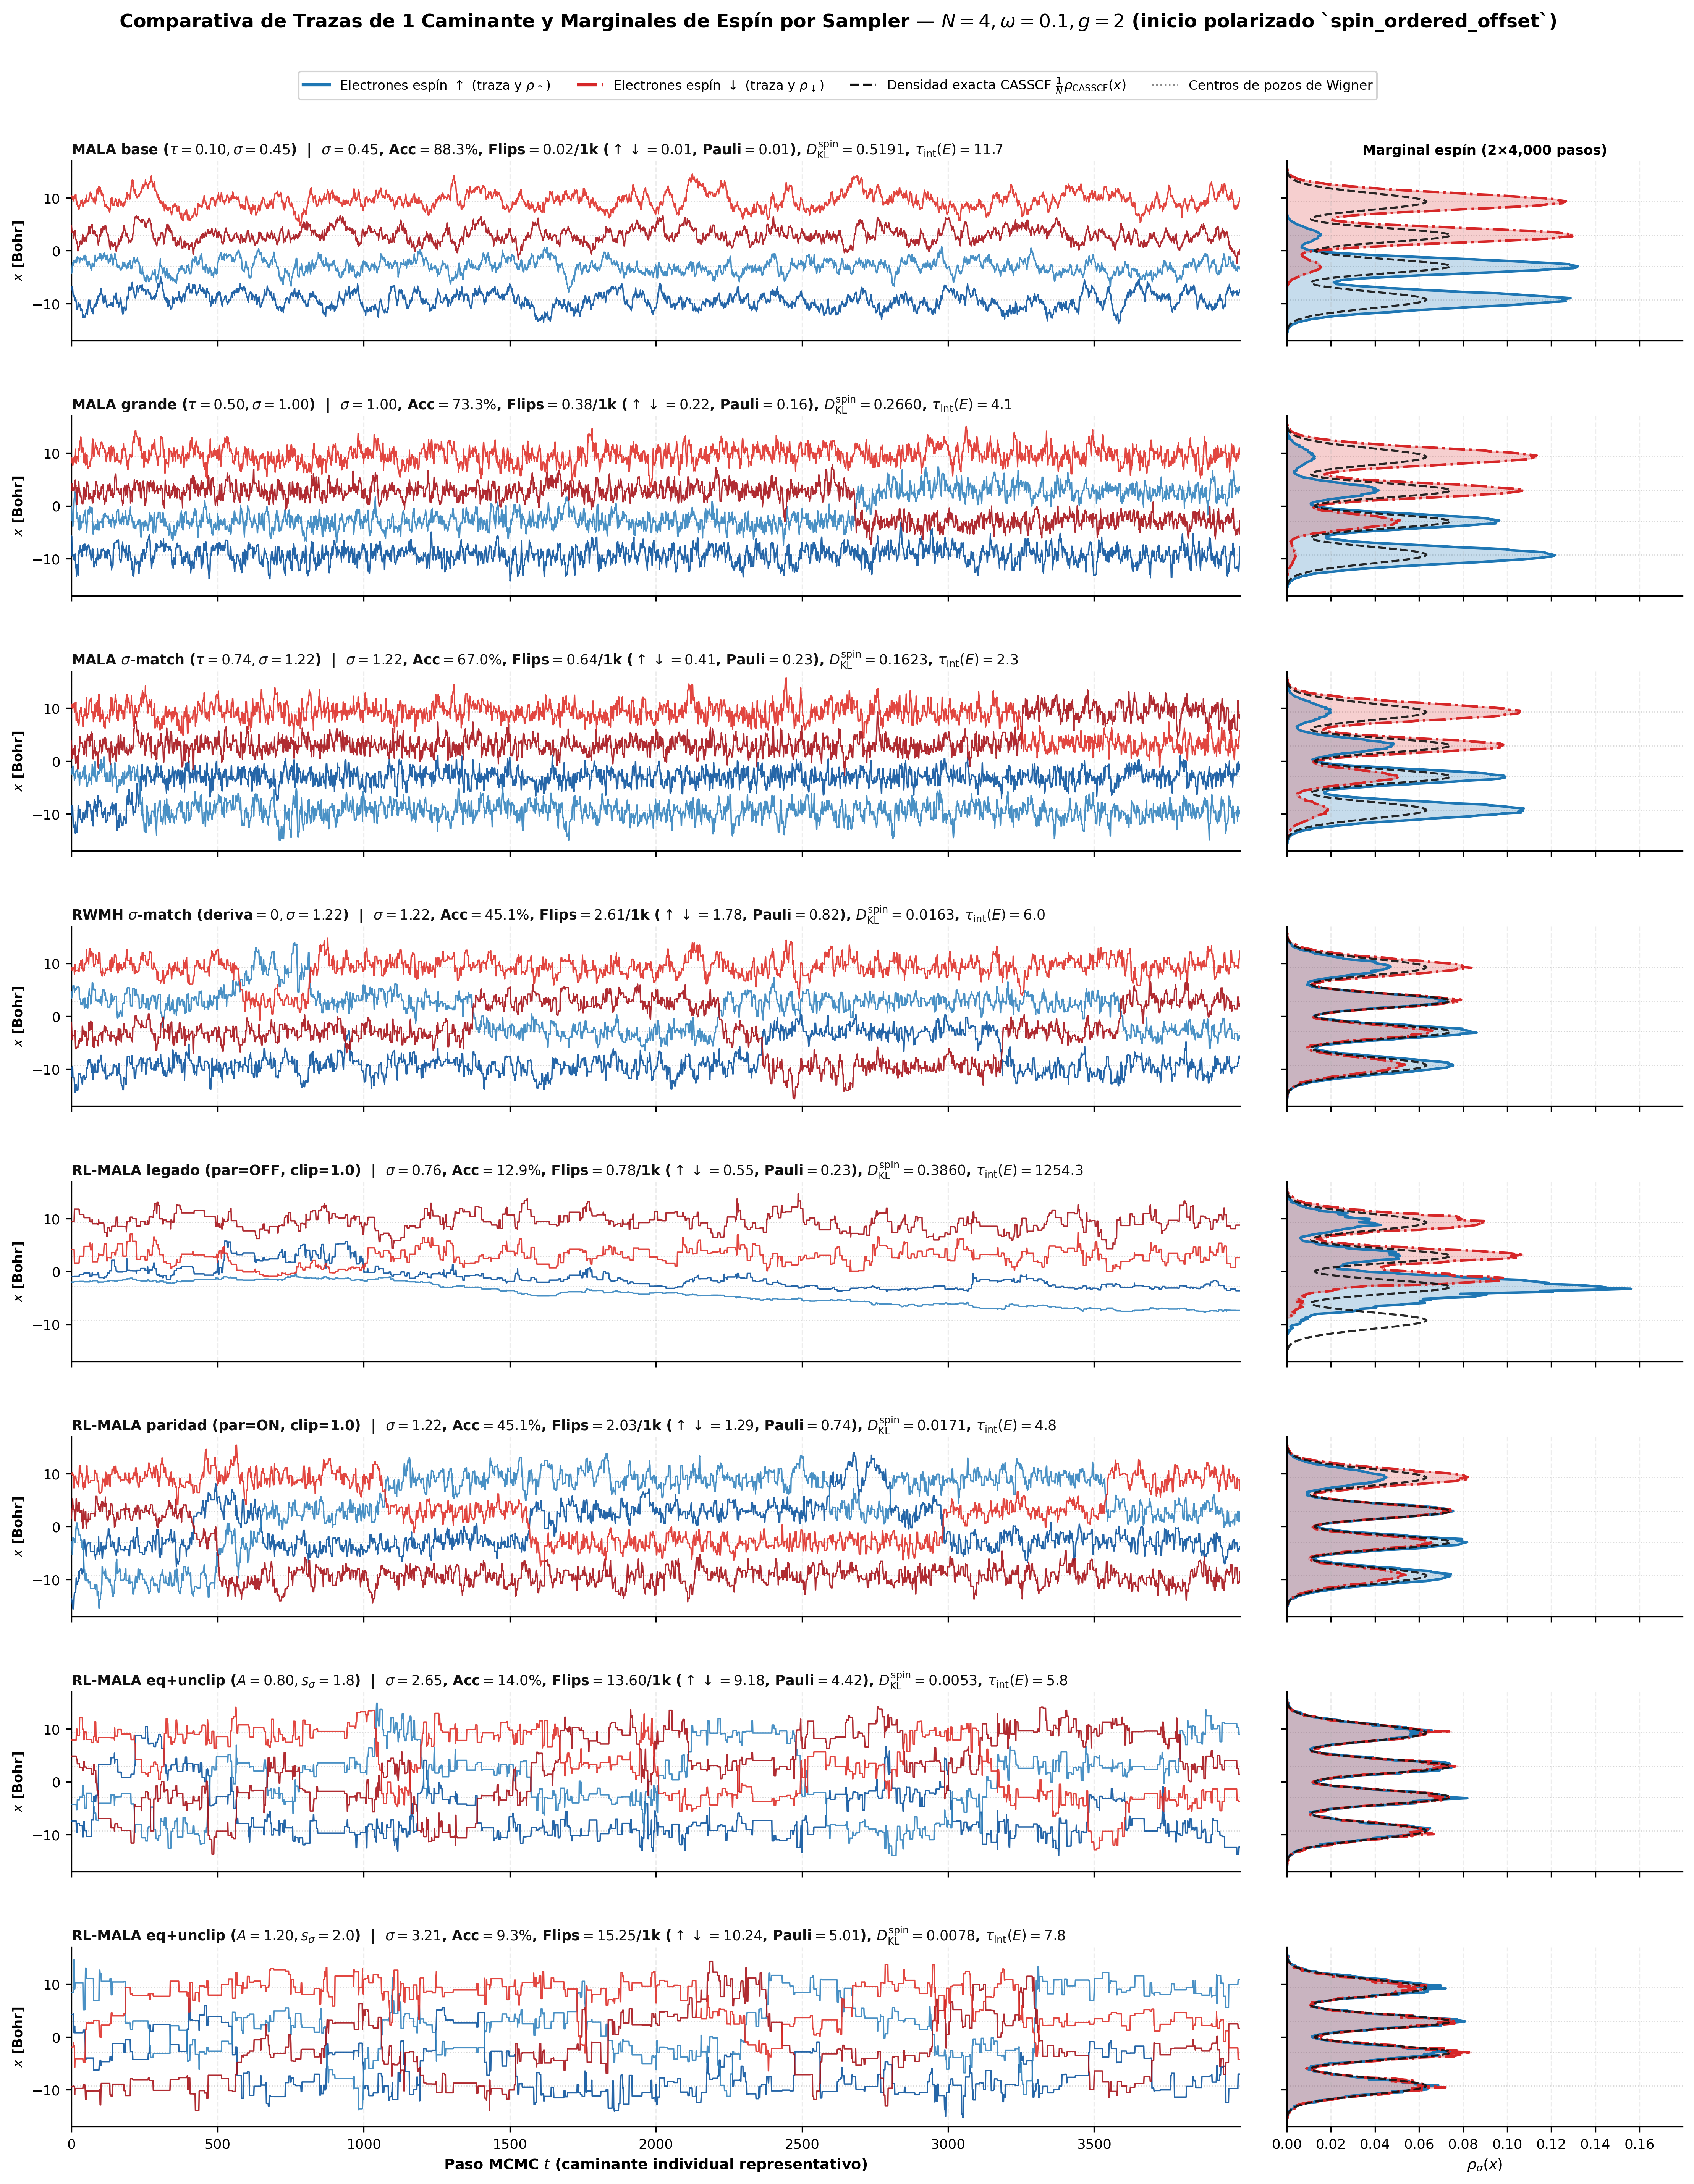
\includegraphics[width=0.98\textwidth]{figures/actor_ablation_N4_g2.0/fig_ablation_traces_and_marginals_N4_w0.1_g2.png}
\caption{\textbf{Trazas de un caminante individual alineadas con sus densidades marginales $\rho_\uparrow(x), \rho_\downarrow(x)$ (B1 + B2, $N=4, \omega=0.1, g=2.0$, corrida local $2\times 4{,}000$ pasos):} \texttt{MALA base} queda atrapado por completo en su sector inicial; \texttt{RWMH($\sigma=1.22$)} difunde suavemente dentro de los pozos con pocos saltos; \texttt{RL-MALA eq+unclip} ($\sigma=2.71\text{--}3.30$) logra numerosos cruces nodales pero exhibe mesetas horizontales en escalera por baja aceptación ($9\%\text{--}14\%$).}
\label{fig:ablation_traces_n4}
\end{figure}

\begin{figure}[H]
\centering
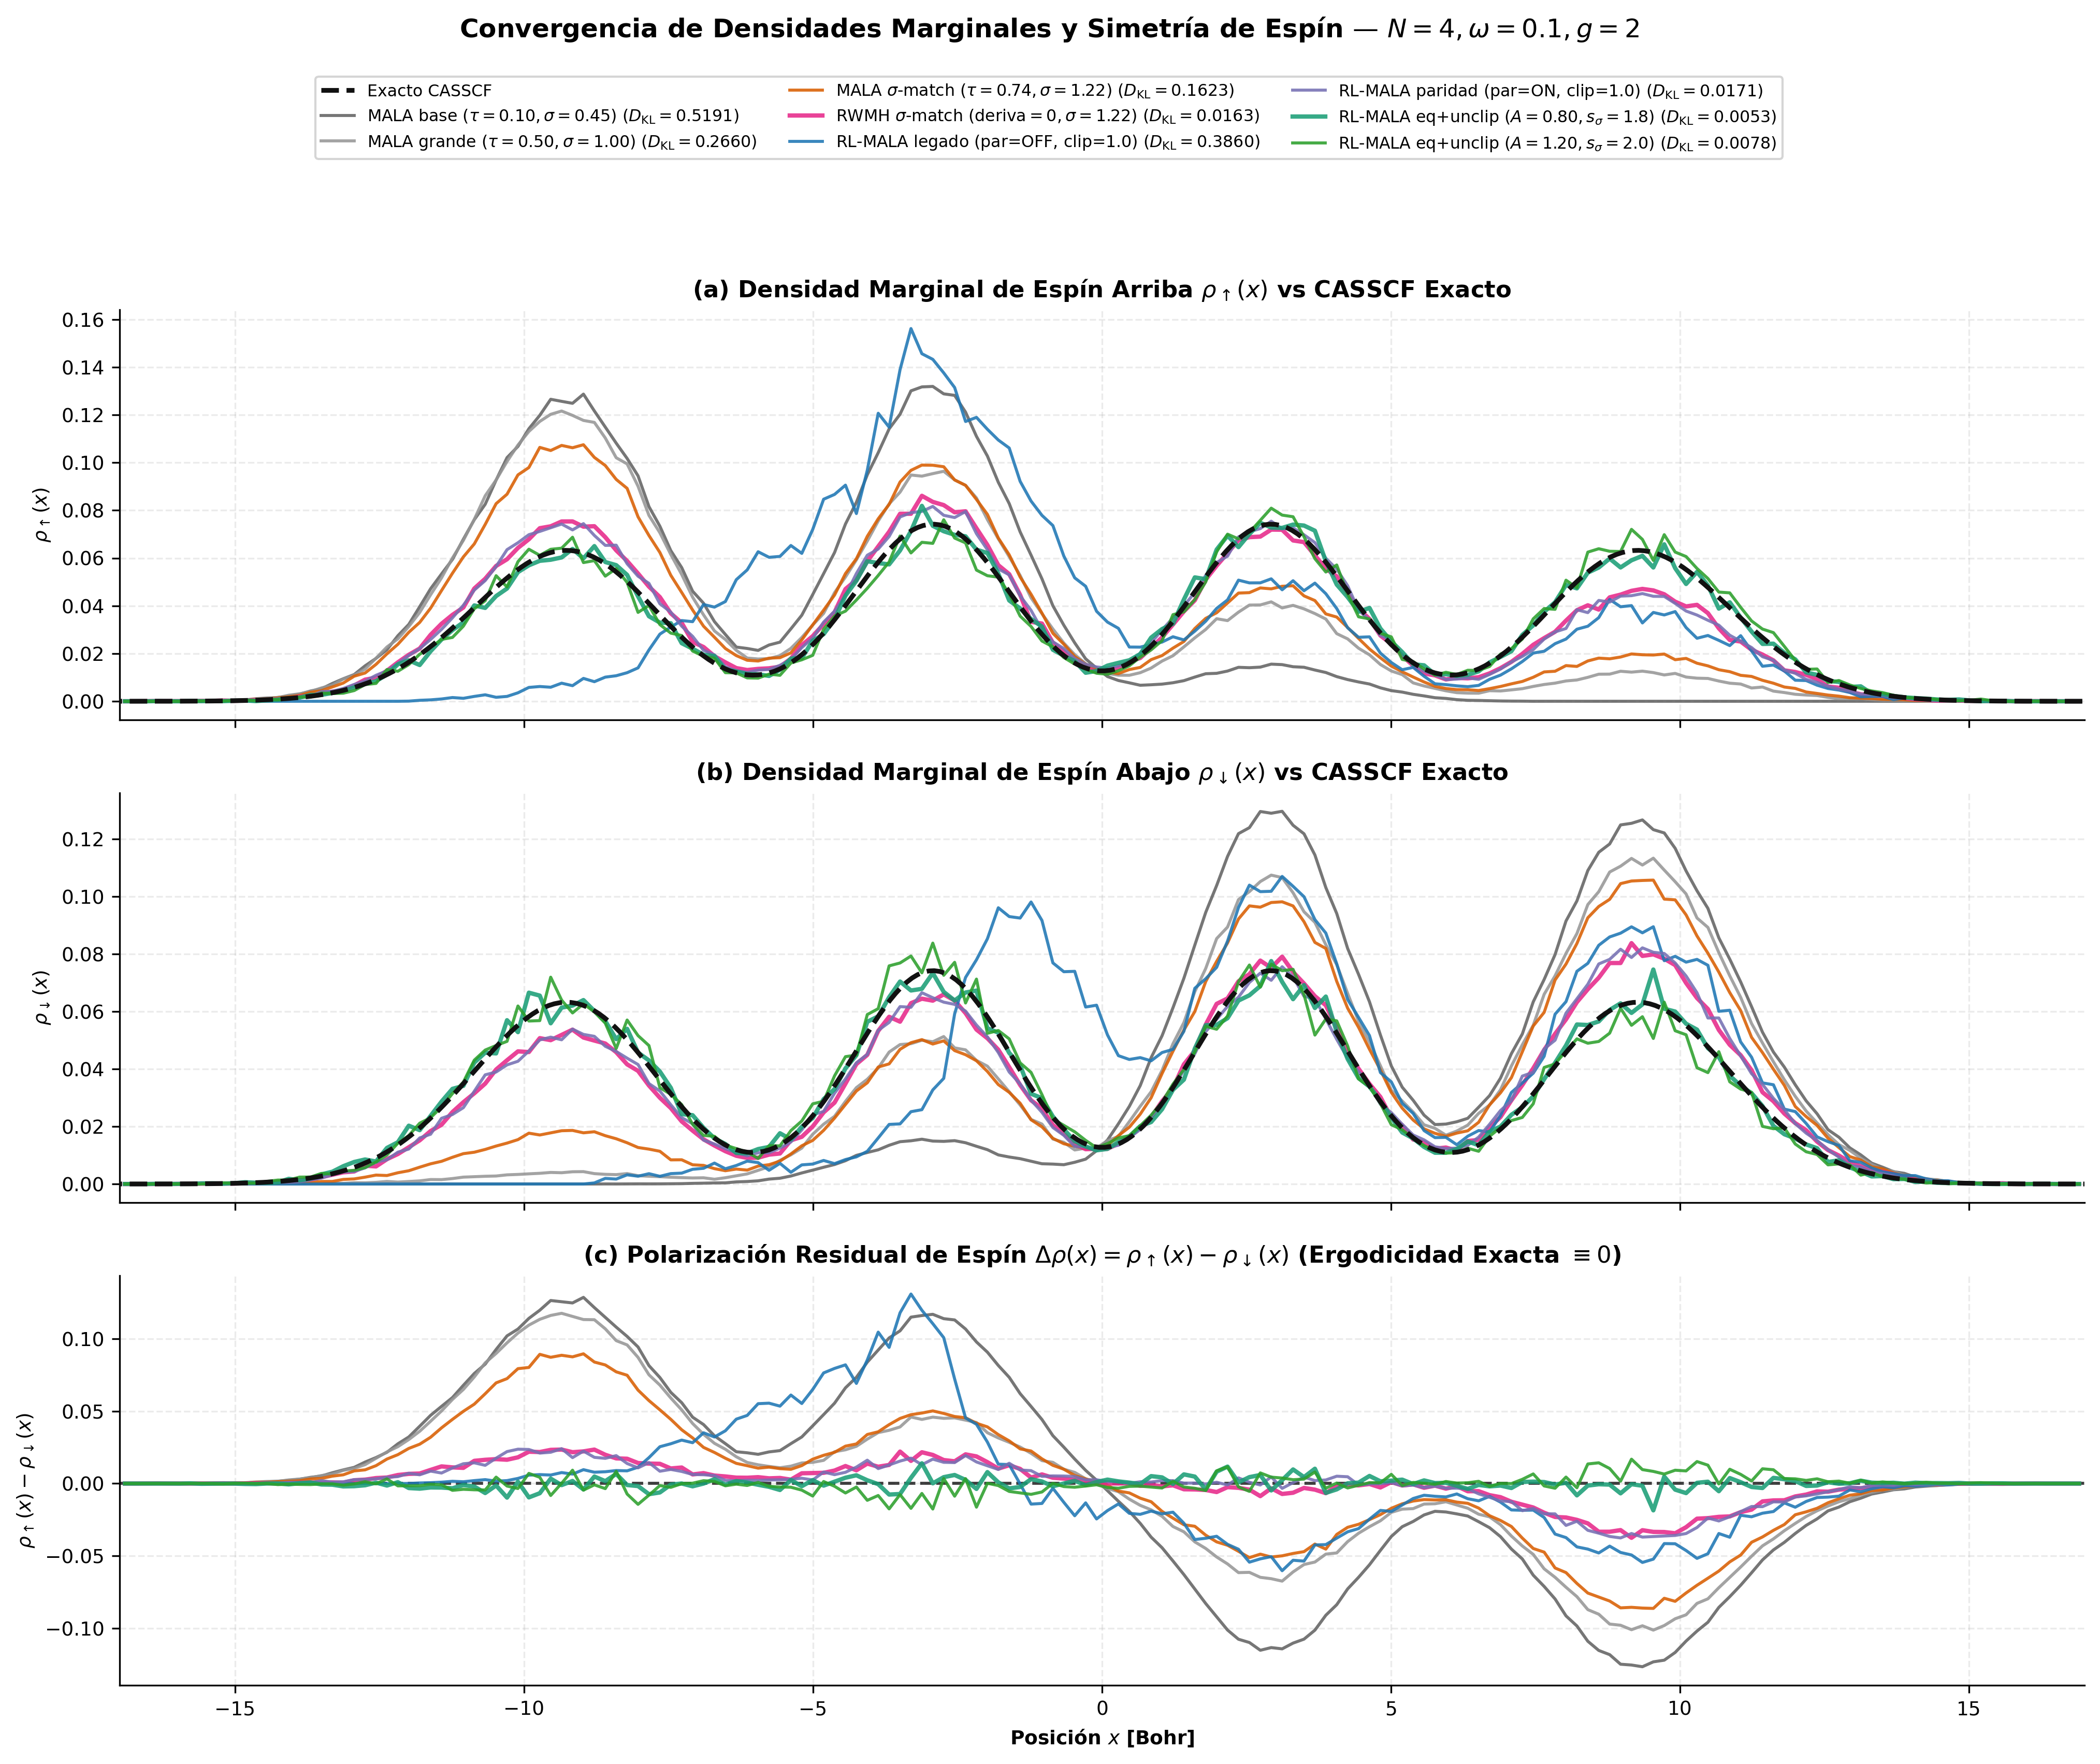
\includegraphics[width=0.98\textwidth]{figures/actor_ablation_N4_g2.0/fig_ablation_marginals_spin_symmetry_N4_w0.1_g2.png}
\caption{\textbf{Simetría de espín $\rho_\uparrow(x)$ vs $\rho_\downarrow(x)$ y error residual respecto a CASSCF exacto ($N=4, \omega=0.1, g=2.0$):} El efecto escalera de \texttt{RL-MALA eq+unclip} ($9\%\text{--}14\%$ de aceptación) se traduce directamente en picos dentados de alta varianza estadística sobre las crestas de densidad, mecanismo que domina $D_{\mathrm{KL}}^{\mathrm{spin}}$ en las corridas largas de Ayler ($3\times 40{,}000$ pasos).}
\label{fig:ablation_marginals_n4}
\end{figure}

\end{document}
